\chapter{Missing higher order uncertainties}
\label{chapter:mhous}
In this chapter we address the dominant source of theory uncertainty in current PDF fits: missing higher order uncertainties (MHOUs). In Sec.~\ref{sec:intro} we explain their origin, then in Sec.~\ref{sec:svn} we revise their standard method of estimation, through scale variation. We then show how to use this to construct a theory covariance matrix (Sec.~\ref{sec:prescrip}), and test the validity of this at NLO against the known NNLO result (Sec.~\ref{sec:valid}). Finally, we present the PDFs including MHOUs (Sec.~\ref{sec:pdfs}).

\section{Introduction}
\label{sec:intro}
PDF fits rely on the comparison of experimental data with theoretical predictions at the partonic level. These predictions are carried out in the framework of perturbation theory, where results are expressed as an expansion in the strong coupling constant, $\alpha_s$. The first non-zero contribution to the expansion is known as ``leading order" (LO), the next is ``next-to-leading order" (NLO), and so on (NNLO, N$^3$LO etc.). Because in the perturbative regime $\alpha_s$ is small (0.11791 $\pm$ 0.00009 \cite{pdg}), corrections from higher orders are increasingly small. Predictions must be directly calculated at each order by considering all the possible contributing Feynman diagrams, and this becomes exponentially more complicated with increasing orders; the cutting edge of calculations is currently at the N$^3$LO level. PDFs are fitted using predictions truncated at a given order, with NNLO PDFs being the modern standard. 

These missing higher order terms in the expansion for theory predictions lead to MHOUs, which are currently the dominant source of uncertainty in PDF fits. We can see that going from LO to NLO to NNLO in Fig.~\ref{fig:pdf_order_comp} that the functional form of the PDF changes, and that the change from LO to NLO is greater than that from NLO to NNLO. MHOUs are currently not included in the PDF uncertainties, justified historically by the claim that they are small compared to experimental contributions to the PDF uncertainty, especially at NNLO. This justification, however, is now on shakier ground with PDF uncertainties dropping as low as 1\% at the electroweak scale. QCD MHOU uncertainties themselves are typically $\mathcal{O}$(1\%)~\cite{Campbell:2017hsr} and, with the current push to N$^3$LO precision, will only become increasingly important as time goes on. 

\begin{figure}[!t]
\centering
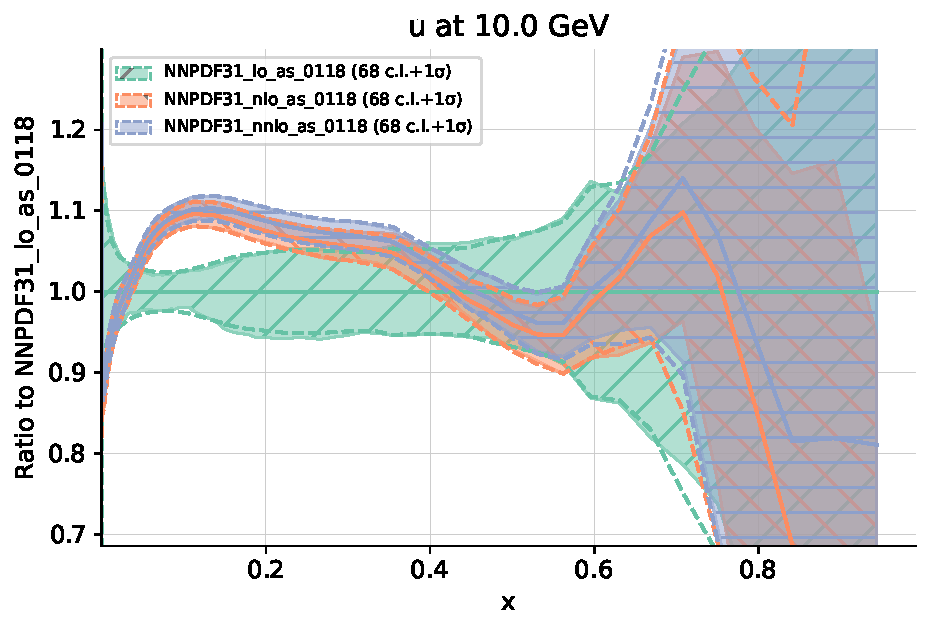
\includegraphics[width=0.49\linewidth]{mhous/plots/pdfscalespecs1_basespecs0_pdfnormalize1_plot_pdfs_u.pdf}
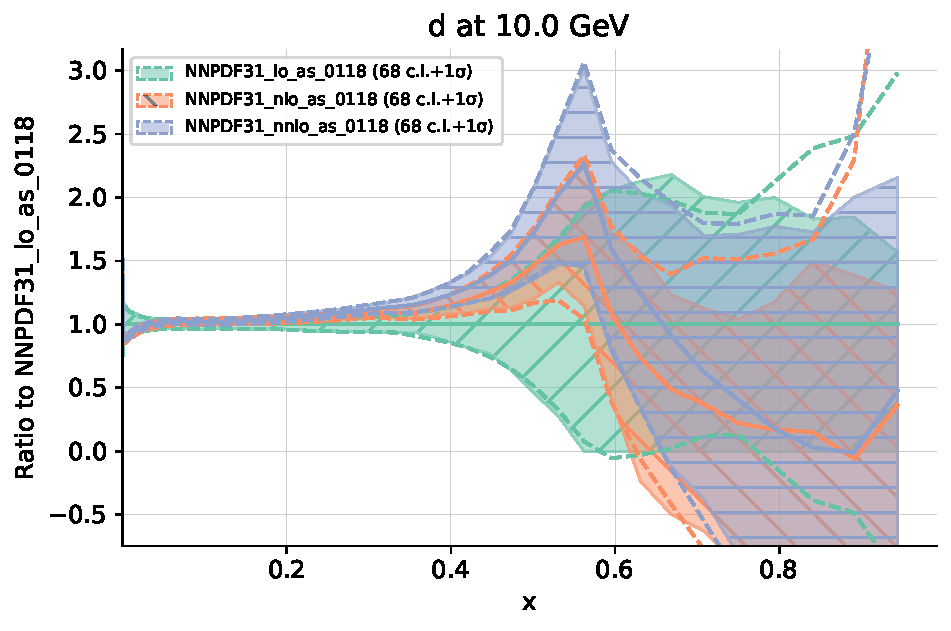
\includegraphics[width=0.49\linewidth]{mhous/plots/pdfscalespecs1_basespecs0_pdfnormalize1_plot_pdfs_d.pdf}\\
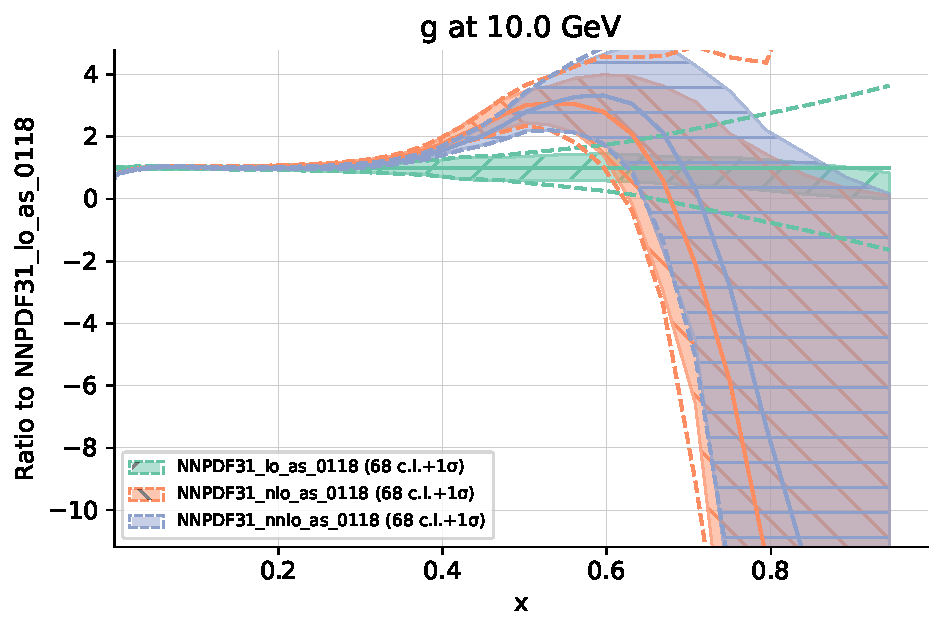
\includegraphics[width=0.49\linewidth]{mhous/plots/pdfscalespecs1_basespecs0_pdfnormalize1_plot_pdfs_g.pdf}
\caption{Comparison of NNPDF3.1 PDFs at different perturbative orders: LO (green); NLO (orange); NNLO (blue). PDFs are normalised to the LO result, and displayed at scale $Q$ = 10 GeV.}
\label{fig:pdf_order_comp}
\end{figure}

In addition to a missing source of per-point uncertainty on each data point, MHOUs can affect a PDF fit more insidiously by impacting on the desired weight of data sets relative to one another; regions of data with high MHOU are naturally to be trusted less when used to determine the PDFs, and so should carry less weight in the fitting process. If MHOUs are included, these data will be deweighted automatically because they will carry higher uncertainty, however in the absence of MHOUs they may impact on a fit to an undesirable degree.

Having established the importance of including MHOUs, in the next section we will go on to develop a formalism for estimating them, and constructing a MHOU covariance matrix.

\section{Scale variation}
\label{sec:svn}

The most popular method for estimating MHOUs is by ``scale variation". This is based on making theoretical predictions at a range of values of the artificial renormalisation ($\mu_R$) and factorisation ($\mu_F$) scales introduced in Chapter~\ref{chapter:background}. The renormalisation group equation (RGE;~\ref{eqn:rge}) and factorisation theorem only hold to all orders in perturbation theory, and in this case varying the scale values will have no effect on any results. However, when the perturbative expansion is truncated, there will be a residual $\mu_R$ and $\mu_F$ dependence which characterises the degree of MHOU. Varying these scales and observing the impact on the predictions can therefore provide an estimate of the MHOUs. 

Although other approaches to estimating MHOUs, based on the current known orders, have been suggested~\cite{Cacciari:2011ze, David:2013gaa, Bagnaschi:2014wea, Bonvini:2020xeo}, we adopted the method of scale variations not only because it is the most widely used, but also because it is the most easily implemented for our purposes. Firstly, the renormalisation group invariance is incorporated automatically, which ensures the MHOUs decrease as the perturbative order increases. Secondly, the scale dependece of $\alpha_s(\mu_R^2)$ and the PDFs is universal to all processes, which is important for PDF fits dealing with a range of interactions. Finally, correlations between data points are implicitly maintained because predictions for different scale values will be smooth functions of kinematics; this ensures that neighbouring regions of phase space will be strongly correlated.

There are, however, some disadvantages. Firstly, the definition of the two scales themselves has been historically approached in various ways, often differently for DIS and hadronic collisions, but also changing over time. Since PDFs use both DIS and hadronic data we need to settle on a consistent approach. Secondly, there is no cut and dry method for determining the range of varied scale choices, and in fact the choice of central scales are themselves to some degree arbitrary; for example, top production processes commonly have both central scales set to the top mass, $m_t$, and DIS processes have both set to Bj\"orken $Q$. Though there is physical motivation for these choices, we could equally well pick 2$m_t$ rather than $m_t$ in the former case, for example. A standard approach is to take the 7-point envelope of the predictions obtained by varying $(\mu_F, \mu_R)$ independently in $\{1/2, 1, 2\}$, excluding $(1/2, 1/2)$ and $(2,2)$. However, for our purposes we do not want a per-point envelope but rather a covariance matrix which retains correlations between data points. We will address both of these drawbacks below. 

Finally, scale variation techniques will not pick up any ``new physics" at higher orders, be it additional colour configurations, singularities or mechanisms of interaction. This is harder to deal with, and requires resummation techniques among other methods. In this work we assume these effects to be less important, and do not address them for the time being.

In the remainder of this section we will review the technique of scale variation, and with it the definitions of $\mu_F$ and $\mu_R$. We will converge on a general formalism that can be applied to both electroproduction and hadroproduction. We will show that there are two independent directions of scale variation and discuss how to combine them, both in single process and multi-process interactions. We will then go on to show how to use this to build a covariance matrix in Sec.~\ref{sec:prescrip}.

\subsection{Renormalisation group invariance}

It is customary when making a theory prediction to pick a renormalisation scale, $\mu_R$, that is indicative of the physical scale of the interaction, $Q$. We will denote this ``central" theory prediction by $T(Q^2)$. In general, a theory prediction at scale $\mu_R$ can be written
$\overline{T}(\alpha_s(\mu_R^2), \mu_R^2/Q^2)$, where we explicitly note that $\alpha_s$ itself depends on the renormalisation scale. From this we can see that
\beq
T(Q^2) \equiv \overline{T}\big(\alpha_s(Q^2), 1 \big).
\eeq
The strong coupling constant satisfies the RGE
\beq \label{eqn:beta}
\mu_R^2 \frac{d^2}{d\mu_R^2}\alpha_s(\mu_R^2) = \beta \big( \alpha_s (\mu_R^2) \big),
\eeq
and we can expand the beta function perturbatively as
\beq 
\beta(\alpha_s) = \beta_0 \alpha_s^2 + \beta_1 \alpha_s^3 
+ \beta_2 \alpha_s^4 + \ldots \, .
\eeq

As discussed in Chapter~\ref{chapter:background}, renormalisation group invariance tells us that a prediction of a physical quantity (such as $\overline{T}$) to all orders must be independent of $\mu_R$, because this scale is unphysical. This means we can write
\beq \label{eqn:rgetbar}
  \mu_R^2 \frac{d}{d \mu_R^2} \overline{T} \lp
  \alpha_s(\mu_R^2), \mu_R^2/Q^2\rp  = 0 .
\eeq

Before proceeding further, we introduce some variables to make the analysis clearer:
\beq \label{eqn:notn}
\mu_R^2 = k Q^2,\qquad t = \ln (Q^2 / \Lambda^2), \qquad \kappa = \ln k = \ln \mu_R^2/Q^2,
\eeq
where $\Lambda$ is the QCD scale. This means $\alpha_s(\mu_R^2)$ is a function of $\ln \mu_R^2/\Lambda^2 = t + \kappa$.

Revisiting Eqn.~\ref{eqn:rgetbar}, we can write this as
\bea \label{eqn:newrge}
	0 & =& \frac{d}{d \kappa} \overline{T}(\alpha_s(t + \kappa), \kappa) \nonumber\\
	& =& \frac{d} {d \kappa} \alpha_s(t + \kappa) \frac{\partial}{\partial \alpha_s} \overline{T}(\alpha_s(t + \kappa), \kappa) \bigg|_\kappa + \frac{\partial}{\partial \kappa} \overline{T}(\alpha_s(t + \kappa), \kappa) \bigg|_{\alpha_s}\nonumber, \\
\eea
assuming that $\overline{T}$ is analytic in $\alpha_s$ and $\kappa$. To simplify this we can use
\beq 
	\frac{d}{d \kappa} \alpha_s(t + \kappa) = \frac{d}{dt} \alpha_s(t + \kappa) = \frac{d}{d \ln \mu_R^2} \alpha_s(t + \kappa) = \beta(\alpha_s(t + \kappa) ) \, ,
\eeq
where we have used the definition of the beta function (Eqn.~\ref{eqn:beta}), and this means that
\beq
	0 = \frac{\partial}{\partial t} \overline{T}(\alpha_s(t + \kappa), \kappa) \bigg|_\kappa + \frac{\partial}{\partial \kappa} \overline{T}(\alpha_s(t + \kappa), \kappa) \bigg|_{\alpha_s} \, .
\eeq
We can now Taylor expand $\overline{T}(\alpha_s, \kappa)$ about the central scale $\mu_R^2 = Q^2 \implies k=1 \implies \kappa = 0$ for fixed $\alpha_s$: 
\bea
  \overline{T}(\alpha_s(t + \kappa), \kappa) &=& \overline{T}(\alpha_s(t + \kappa), 0)\nonumber\\&&\qquad\qquad +\kappa \frac{\partial}{\partial \kappa} \overline{T}(\alpha_s(t + \kappa), 0) \bigg|_{\alpha_s} + \half \kappa^2 \frac{\partial^2}{\partial \kappa^2} \overline{T}(\alpha_s(t + \kappa, 0)\bigg|_{\alpha_s} + \ldots \qquad \nonumber \\.
\eea
Then, using Eqn.~\ref{eqn:newrge}, we can replace $\frac{\partial}{\partial \kappa}$ with
$-\frac{\partial}{\partial t}$, and write
\bea \label{eqn:trelation}
\overline{T}(\alpha_s(t + \kappa), \kappa) &=& \overline{T}(\alpha_s(t + \kappa), 0) - \kappa \frac{\partial}{\partial t} \overline{T}(\alpha_s(t + \kappa), 0) \bigg|_\kappa \nonumber\\ &+& \half \kappa^2  \frac{\partial^2}{\partial t^2} \overline{T}(\alpha_s(t + \kappa), 0)\bigg|_\kappa + \ldots \nonumber\\
&=& T(t + \kappa) - \kappa \frac{d}{dt} T(t + \kappa) + \half \kappa^2  \frac{d^2}{dt^2} T(t + \kappa)+\ldots\>.
\eea
This tells us how to find a scale varied theoretical prediction, $\overline{T}$, in terms of the $t$ dependence of the central prediction, $T$. Furthermore, we can express this $t$ dependence as an $\alpha_s$ dependence using
\beq
\frac{d}{dt} T(t) = \frac{d \alpha_s(t)}{dt} \frac{\partial}{\partial \alpha_s} \overline{T}(\alpha_s(t), 0) = \beta(\alpha_s(t)) \frac{\partial}{\partial \alpha_s} \overline{T}(\alpha_s(t), 0).
\eeq
Noting that $\beta(\alpha_s) = \mathcal{O}(\as^2)$, we see that 
$\frac{1}{T} \frac{dT}{dt}
= \mathcal{O}(\alpha_s)$ and $\frac{1}{T} \frac{d^2T}{dt^2} =
\mathcal{O}(\alpha_s^2)$ etc. The pattern follows that every time a derivative is taken with respect to $t$ you pick up a power of $\alpha_s$ as a consequence of the chain rule in differentiating. Looking back at Eqn. \ref{eqn:trelation} it is clear that each power of $\kappa$ is associated with a power of $\alpha_s$. Expressing the theory prediction perturbatively as
\be
T = \alpha_sT_{\text{LO}} + \alpha_s^2 T_{\text{NLO}} + \alpha_s^3 T_{\text{NNLO}} + \ldots\> ,
\ee
we can match powers of $\alpha_s$ in Eqn. \ref{eqn:trelation} to obtain the expressions
\begin{align} \label{eqn:theoryshifts}
\begin{split}
	\overline{T}_{\text{LO}}(\alpha_s(t + \kappa), \kappa) & = T_{\text{LO}}(t + \kappa), \\
	\overline{T}_{\text{NLO}}(\alpha_s(t + \kappa), \kappa) & = T_{\text{NLO}}(t + \kappa) - \kappa\smallfrac{d}{dt}{T}_{\text{LO}}(t + \kappa), \\
	\overline{T}_{\text{NNLO}}(\alpha_s(t + \kappa), \kappa) & = T_{\text{NNLO}}(t + \kappa) - \kappa\smallfrac{d}{dt}{T}_{\text{NLO}}(t + \kappa) \\
	&+ \half\kappa^2  \smallfrac{d^2}{dt^2}{T}_{\text{LO}}(t + \kappa).
\end{split}
\end{align}

The difference between the scale varied prediction and the central scale prediction,
\be
\Delta(t,\kappa) = \overline{T}(\alpha_s(t + \kappa), \kappa) - T(t) \, .
\ee
can be used to estimate the MHOU. From Eqn.~\ref{eqn:theoryshifts} we find the explicit expressions for the theory uncertainties
\be 
\begin{split}
\Delta_{\text{LO}}(t,\kappa) & = T_{\text{LO}}(t + \kappa)-T_{\text{LO}}(t), \\
{\Delta}_{\text{NLO}}(t,\kappa) & = (T_{\text{NLO}}(t + \kappa) - \kappa\smallfrac{d}{dt}{T}_{\text{LO}}(t + \kappa))-T_{\text{NLO}}(t), \\
{\Delta}_{\text{NNLO}}(t, \kappa) & = (T_{\text{NNLO}}(t + \kappa) - \kappa\smallfrac{d}{dt}{T}_{\text{NLO}}(t + \kappa) \\
&+ \half\kappa^2  \smallfrac{d^2}{dt^2}{T}_{\text{LO}}(t + \kappa))-T_{\text{NNLO}}(t) \, .
\end{split}
\ee
At LO we can see that the uncertainty results entirely from the choice of $\kappa$, in other words of $\mu_R$ in the $\alpha_s$ evaluation. At NLO we can see that the leading part of $T_{\text{NLO}}(t + \kappa)$ is subtracted off by the $\mathcal{O}(\kappa)$ term, meaning that the uncertainty is reduced with respect to LO. At NNLO, in addition, the $\mathcal{O}(\kappa^2)$ term subtracts off the subleading dependence of $T_{\text{NNLO}}(t + \kappa) - \kappa\smallfrac{d}{dt}{T}_{\text{NLO}}(t + \kappa)$, and so the uncertainty is yet smaller. This pattern of decreased scale variation uncertainties with increased perturbative order reflects our general understanding of the behaviour of MHOUs.

It is also apparent that the size of MHOU depends on the value of $\kappa$, in other words on the size of scale variation. This introduces a degree of arbitrariness into MHOU estimation, with the historical empirical range of choice being $\kappa \in [-\ln 4, \ln 4]$. In practice, we must investigate the dependence of $\Delta$ on $\kappa$, using validation at lower orders against known higher orders to converge on a suitable prescription.  This will be addressed in Sec.~\ref{sec:prescrip}. 

We will now go on to show how RG invariance can be applied to processes involving hadrons, where the partonic cross section is also convolved with a PDF. We will show that in this scenario there are two independent scales, and thus two independent sources of MHOU: one from the $\alpha_s$ dependence in the hard cross section; the other from the anomalous dimensions in the PDF evolution.

\subsection{Scale variation in partonic cross sections}
\label{subsec:svpartonic}
We will start with DIS, where there is only one hadron then move to the case of hadron-hadron collisions, such as those carried out at the LHC. In each case we will consider RG invariance to find an expression for $\mu_R$ variation in the partonic observable, for the case where the PDF is evaluated at the physical scale. Scale variation in PDF evolution, i.e. the $\mu_F$ variation, will be addressed in the next section.
\subsubsection{Deep Inelastic Scattering}
For DIS processes, theory predictions are of the structure functions discussed in Chapter~\ref{chapter:background}. These can be expressed as a convolution of a parton level coefficient, $C$, with a PDF, $f$:
\be 
\label{eqn:strfn}
F(Q^2) = C(x, \alpha_s(Q^2)) \otimes f(x, Q^2),
\ee
where $\otimes$ is a convolution in the momentum fraction, $x$, and there is an implicit sum over parton flavours. There will be a MHOU in $F$ due to truncating the coefficient function, $C$, to fixed perturbative order.  We can estimate this by keeping the PDF scale (or factorisation scale) fixed and varying the renormalisation scale in $C$. This will result in a scale-varied structure function,
\be
    \overline{F}(Q^2, \mu_R^2) = \overline{C}(\alpha_s(\mu_R^2), \mu_R^2/Q^2)\otimes f(Q^2)\, ,
\ee
where we have made the $x$-dependence implicit and the scale dependence explicit in the coefficient function. We can use the quantities defined in Eqn.~\ref{eqn:notn} to write this as
\be 
    \overline{F}(t, \kappa) = \overline{C}(\alpha_s(t + \kappa), \kappa)\otimes f(t).
\ee
We know that the structure function, an observable, is RG invariant, and, because we are keeping the factorisation scheme fixed, the PDF is independent of $\mu_R$. This means that the coefficient functions must also obey RG invariance, and so in a parallel with Eqn.~\ref{eqn:trelation} we can write
\be	
\overline{C}(\alpha_s(t + \kappa), \kappa) = C(t + \kappa) - \kappa \smallfrac{d}{dt} C(t + \kappa) + \half \kappa^2  \smallfrac{d^2}{dt^2} C(t + \kappa)+\ldots,
\ee
where, like before, we denote the central scale quantities without a bar. In order to evaluate the derivatives, note that the coefficient function can be expressed as a perturbative expansion in $\alpha_s$,
\be 
C(t) = c_0 + \alpha_s(t) c_1 + \alpha_s^2(t) c_2 + \alpha_s^3(t) c_3 +\ldots, 
\ee
and that $\smallfrac{d}{dt}\alpha_s(t,\kappa) = \beta(\alpha_s(t, \kappa)$, where the beta function also admits the expansion in Eqn.~\ref{eqn:beta}. Explicitly, this leads us to
\be 
\begin{split}
\smallfrac{d}{dt}{C}(t) & = \alpha_s^2(t) \beta_0 c_1+ \alpha_s^3(t) (\beta_1c_1+2\beta_0c_2) + \ldots,\\
\smallfrac{d^2}{dt^2}{C}(t) & = 2\alpha_s^3(t) \beta_0^2 c_1+ \ldots,
\end{split}
\ee 
resulting in the perturbative expression for $\mu_R$ variation of $C$:
\be 
\begin{split}
\overline{C}(\alpha_s(t + \kappa), \kappa) = c_0 &+ \alpha_s(t + \kappa) c_1 + \alpha_s^2(t + \kappa) (c_2 - \kappa \beta_0 c_1)\\ 
&+\alpha_s^3(t + \kappa)\big(c_3-\kappa (\beta_1c_1+2\beta_0c_2)+ \kappa^2 \beta_0^2 c_1\big) + \ldots \, .
\end{split}
\ee 
Using Eqn.~\ref{eqn:strfn} we finally get an expression for the $\mu_R$ variation of $F$:
\be 
\begin{split}
\overline{F}(t, \kappa) = c_0\otimes f(t) &+ \alpha_s(t + \kappa) c_1\otimes f(t) + \alpha_s^2(t + \kappa)  \lp c_2 - \kappa \beta_0 c_1 \rp \otimes f(t)\\ 
&+\alpha_s^3(t + \kappa) \lp c_3-\kappa (\beta_1c_1+2\beta_0c_2)+ \kappa^2 \beta_0^2 c_1 \rp \otimes f(t) + \ldots\>. 
\end{split}
\ee
In practice, when predicting scale varied observables, using these equations is relatively straightforward. Because the coefficients, $c_i$ and $\beta_i$, are already known to some order, the workflow consists of some basic algebra to create the new, scale varied, coefficients at each order from the central-scale coefficients at the surrounding orders.

\subsubsection{Hadron-hadron collisions}
Hadron-hadron collisions can be considered in a similar way to DIS, the difference being that the observable cross section, $\Sigma$, depends on two PDFs, one for each of the hadrons:
\be 
    \Sigma(t) = H(t)\otimes( {f}(t)\otimes  {f}(t)) \, ,
\ee
where $H$ is the parton level cross section and this time we have used $t = \ln (Q^2 / \Lambda^2)$ from the outset. Once again, there is an implicit sum over parton flavours. As before, we can vary $\kappa = \ln (\mu^2/Q^2)$ in $H$ whilst keeping $f$ fixed, so that
\be \label{eqn:svarhadronic}
  \overline{\Sigma}(t,\kappa) = \overline{H} (\as(t+\kappa), \kappa)\otimes(f(t)\otimes f(t)),
\ee 
where
\be 
\overline{H}(\alpha_s(t), \kappa) = H(t) - \kappa \smallfrac{d}{dt} H(t) + \half \kappa^2  \smallfrac{d^2}{dt^2} H(t)+\ldots\>. 
\ee
Because hadron-hadron collisions involve a range of processes, we consider a generic process starting at $O(\alpha_s^n)$ for $n \in \mathbb{Z}$, so that
\be 
H(t) = \alpha_s^n(t)h_0 + \alpha_s^{n+1}(t)h_1 + \alpha_s^{n+2}(t)h_2+ \ldots\>.
\ee
Once again using $\smallfrac{d}{dt}\alpha_s(t,\kappa) = \beta(\alpha_s(t, \kappa)$ and Eqn.~\ref{eqn:beta} we arrive at
\begin{equation}
\begin{split}
\smallfrac{d}{dt}{H}(t) & = n\alpha_s^{n-1}(t)\beta(\alpha_s) h_0 + (n+1)\alpha_s^n(t)\beta(\alpha_s) h_1 + \ldots \\
&= \alpha_s^{n+1} n \beta_0 h_0 + \alpha_s^{n+2} (n \beta_1 h_0 + (n+1) \beta_0 h_1) + \ldots\\
\smallfrac{d^2}{dt^2}{H}(t) & = \alpha_s^{n+2} n(n+1) \beta_0^2 h_0 + \ldots.
\end{split}
\end{equation}
Overall, to evaluate $\overline{\Sigma}$ we can therefore use Eqn.~\ref{eqn:svarhadronic} along with 
\bea  \label{eqn:svarH}
    \overline{H}(\alpha_s, \kappa) &=& \alpha_s^n h_0 + \alpha_s^{n+1} (h_1 - \kappa n \beta_0 h_0) \nonumber\\ &+&\alpha_s^{n+2} (h_2 - \kappa(n \beta_1 h_0 + (n+1) \beta_0 h_1) \nonumber\\ &&\qquad+ \half \kappa^2 n(n+1) \beta_0^2 h_1) + \ldots .
\eea
Again, to evaluate the scale varied cross section, all that is needed is to modify the coefficients at each order using those at the central scale for the surrounding orders.
\subsection{Scale variation in evolution of PDFs}
We now turn to the effects of scale variation in the PDFs themselves. This is a crucial contribution to MHOUs because the PDFs are common to predictions for all processes, and therefore responsible for widespread correlations in uncertainty. MHOUs in the PDFs arise from the truncation of the perturbative expansion of the splitting functions (or, in Mellin space, the anomalous dimensions) in the DGLAP evolution equations (Eqn.~\ref{eqn:DGLAP}) discussed in Chapter~\ref{chapter:background}. The scale evolution of the PDFs can be encapsulated in Mellin space in the equation
\be \label{eqn:mellindglap}
	\mu_F^2 \frac{d}{d \mu_F^2} f(\mu_F^2) = \gamma(\alpha_s(\mu_F^2)) f(\mu_F^2)\, ,
\ee
where the parton flavour indices are left implicit and the anomalous dimension, $\gamma$, can be expressed as an expansion in $\alpha_s$ as
\be  \label{eqn:anomdimexp}
\gamma(t) =  \alpha_s(t) \gamma_0 + \alpha_s^2(t) \gamma_1^2  + \alpha_s^3(t) \gamma_2^3 + \cdots .
\ee
Note that we refer to a separate factorisation scale, $\mu_F$, distinct from the renormalisation scale, $\mu_R$, in the previous section. This is because each scale is associated with a separate RGE and they are therefore independent; to explore the full space of scale variations they need to be considered separately. 

To solve for the PDF, we can integrate Eqn.~\ref{eqn:mellindglap} to give
\be \label{eqn:pdfint}
	f(\mu_F^2) = \text{exp}\bigg(\int_{\mu_0}^{\mu_F^2} \frac{d \mu^{2}}{\mu^{2}} \gamma(\alpha_s(\mu^{2}))\bigg) f_0 \, ,
\ee
where $f_0$ is the PDF at the initial scale, $\mu_0$. Note that the LHS is independent of the choice of $\mu_0$. To consider the effect of scale variations on the PDF, we can proceed similarly to Sec.~\ref{subsec:svpartonic}, defining 
\beq \label{eqn:notn2}
\mu_F^2 = k Q^2,\qquad t = \ln (Q^2 / \Lambda^2), \qquad \kappa = \ln k = \ln \mu_F^2/Q^2,
\eeq
and finding the scale varied anomalous dimension
\be \label{eqn:svanomdim}
	\overline{\gamma}(\alpha_s(t), \kappa) = \gamma(t) - \kappa
        \smallfrac{d}{dt}{\gamma}(t) + \half \kappa^2
        \smallfrac{d^2}{dt^2}{\gamma}(t) + \cdots .
\ee
Once again we can use the beta function expansion (Eqn.~\ref{eqn:beta}) alongside Eqn.~\ref{eqn:anomdimexp} to give
\bea \label{eqn:anomdimresult}
    \overline{\gamma}(\alpha_s(t + \kappa), \kappa) &=& \alpha_s(t+\kappa) \gamma_0 + \alpha_s^2(t+\kappa) (\gamma_1 - \kappa \beta_0 \gamma_0) \nonumber\\ &+& \alpha_s^3(t+\kappa) (\gamma_2 - \kappa (\beta_1 \gamma_0 + 2 \beta_0 \gamma_1) + \kappa^2 \beta_0^2 \gamma_0) \nonumber\\ &+& \cdots \, ,
\eea
which has the same form as Eqn.~\ref{eqn:svarH} upon setting $n=1$. We can use this equation to estimate MHOUs in PDFs, which can be done by refitting the PDF at each scale choice using different anomalous dimensions. This method has been applied in previous analyses~\cite{Martin:1990fq, Virchaux:1991jc, Ridolfi:1999vr}, but the process of refitting the PDFs is computationally intensive and so we would like to avoid having to do this if possible. Instead, we can look directly at the PDF level and consider evaluating the PDFs themselves at different scales, as was done in \cite{Altarelli:2008aj}.  

We can define the scale varied PDF as that obtained by varying the scale in the anomalous dimension,
\be
\overline{f}(\as(t + \kappa), \kappa) = \text{exp}\bigg(\int_{t_0}^t dt' \overline{\gamma}(\alpha_s(t' + \kappa), \kappa)\bigg) f_0 \, 
\ee
Shifting integration variable $t' \to t'- \kappa$ whilst redefining the initial scale, we can then apply Eqn.~\ref{eqn:svanomdim} and expand the exponential, {\it i.e.}
\bea
\overline{f}(\as(t + \kappa), \kappa) &=& \text{exp}\bigg(\int_{t_0}^{t+\kappa} dt' \overline{\gamma}(\alpha_s(t'), \kappa)\bigg) f_0 \nonumber\\
&=& \exp\lp \lc \int_{t_0}^{t + \kappa} dt' \gamma(t')\rc  - \kappa  \gamma(t + \kappa) + \half \kappa^2 \frac{d}{dt} {\gamma}(t + \kappa) + \ldots \rp \nonumber\\
&& \times \exp\lp \kappa  \gamma(t_0) - \half \kappa^2 \frac{d}{dt} {\gamma}(t_0) + \ldots \rp f_0 \\
&=& \lc 1 - \kappa \gamma(t + \kappa) + \half \kappa^2
    (\gamma^2(t + \kappa)+\frac{d}{dt}{\gamma}(t + \kappa)) + \ldots
    \rc \nonumber\\
&& \times \exp\lp \int_{t_0}^{t + \kappa} dt' \gamma(t')\rp \exp\lp \kappa  \gamma(t_0) - \half \kappa^2 \frac{d}{dt} {\gamma}(t_0) + \ldots \rp f_0 \nonumber \, .
\eea
We can absorb the factor resulting from variation of $t_0$ into the initial PDFs, $f_0$, so that $\exp\lp \kappa  \gamma(t_0) - \half \kappa^2 \frac{d}{dt} {\gamma}(t_0) + \ldots \rp f_0 \to f_0$. Then, noting also that $\exp\lp \int_{t_0}^{t + \kappa} dt' \gamma(t')\rp f_0 = f(t + \kappa)$, we end up with the result
\be \label{eqn:pdfvarresult}
\overline{f}(\as(t + \kappa), \kappa) = \lc 1 - \kappa \gamma(t + \kappa) + \half \kappa^2
    (\gamma^2(t + \kappa)+\frac{d}{dt}{\gamma}(t + \kappa)) + \ldots
    \rc f(t+ \kappa) \, .
\ee
This result, which comes from varying the scale at which the PDF is evaluated, is equivalent to the result which comes from varying the scale in the anomalous dimension, Eqn.~\ref{eqn:anomdimresult}. This is because there is only one RGE and therefore only one scale which the PDF depends on. Furthermore, note that Eqn.~\ref{eqn:pdfvarresult} shows us that the scale dependence can be factorised out of the PDF. This means we are free to instead factor it into the parton level coefficient function, which will always appear convolved with the PDF. This is useful when making a scale varied prediction when only a central PDF is available, and has been used in the past to make predictions for new LHC processes (e.g. Higgs production~\cite{deFlorian:2016spz}). However, in the case where we also want to consider $\mu_R$ variation in the coefficient function, the two scale variations will be mixed up, and this can lead to a complicated interplay, especially in the presence of heavy quark effects. In this work we adopt the method of scale variation for PDFs by using Eqn.~\ref{eqn:pdfvarresult}. 

\subsection{Varying two scales together}
We now consider the simultaneous variation of $\mu_R$ in the parton level observable and $\mu_F$ in the PDFs, in order to explore the full range of scale variation space. We will derive formulae for scale variation up to NNLO which are needed to construct a MHOU covariance matrix. 

For a DIS process we can write the double-scale-varied structure function as
\be \label{eqn:doublesv}
\overline{F}(Q^2, \mu_F^2, \mu_R^2) = \overline{C}(\alpha_s(\mu_R^2), \mu_R^2/Q^2) \otimes \overline{f}(\alpha_s(\mu_F^2), \mu_F^2/Q^2).
\ee
Similarly to before, we can define the variables
\beq \label{eqn:notn3}
\mu_{(F/R)}^2 = k_{(F/R)} Q^2,\qquad \kappa_{(F/R)} = \ln k_{(F/R)}, \qquad t_{(F/R)} = t + \kappa_{(F/R)}
\eeq
and use them to write the structure function as
\be
    \overline{F}(t, \kappa_F, \kappa_R) = \overline{C}(t_R, \kappa_R)
    \overline{f}(t_F, \kappa_F).
\ee
We then need to apply the equations for the scale varied PDFs and coefficient functions from the previous section, 
\be 
\begin{split}
    &\overline{f} (t_F, \kappa_F) = f(t_F) - \kappa_F
  \smallfrac{d}{dt}{f}(t_F) + \half \kappa_F^2
  \smallfrac{d^2}{dt^2}{f}(t_F) + ... \, , \\ 
    &\overline{C} (t_R, \kappa_R) = C(t_R) - \kappa_R
  \smallfrac{d}{dt}{C}(t_R) + \half \kappa_R^2
  \smallfrac{d^2}{dt^2}{C}(t_R) + ...   \, ,
\end{split}    
\ee
and use the fact that $\smallfrac{\partial}{\partial t} \sim \mathcal{O}(\alpha_s)$ to see that
\bea
    \overline{F}(t, \kappa_F, \kappa_R) 
    &=& C(t_R)f(t_F) - \lp \kappa_F C(t_R) \smallfrac{d}{dt}{f} (t_F)
    + \kappa_R \smallfrac{d}{dt}{C}(t_R) f(t_F) \rp  \nonumber\\
    &&\qquad + \half\Big(  \kappa_F^2
    C(t_R) \smallfrac{d^2}{dt^2} f(t_F)  
    + 2\kappa_R \kappa_F
    \smallfrac{d}{dt}{C}(t_R)\smallfrac{d}{dt}{f}(t_F) \nonumber\\
    &&\qquad \qquad +
    \kappa_R^2 \smallfrac{d^2}{dt^2}{C}(t_R)f(t_F)\Big) +
    \mathcal{O}(\alpha_s^3) \, . 
\eea
Taking a closer look, and comparing to Eqn.~\ref{eqn:doublesv}, we can write this in terms of partial derivatives of $F$:
\bea
    \overline{F}(t, \kappa_F, \kappa_R)  &=& F(t_F,t_R) - \bigg( \kappa_F\ \frac{\partial F}{\partial t_F}\bigg|_{t_R} + \kappa_R\ \frac{\partial F}{\partial t_R}\bigg|_{t_F} \bigg) \nonumber\\
    &&\qquad+ \half \bigg( \kappa_F^2 \frac{\partial^2 F}{\partial t_F^2}\bigg|_{t_R} +  2 \kappa_F \kappa_R \frac{\partial^2 F}{\partial t_F \partial t_R} \nonumber \\ &&\qquad +  \kappa_R^2 \frac{\partial^2 F}{\partial t_R^2}\bigg|_{t_F} \bigg)  + \cdots \, .    
\eea
Considering this expression, we can think of $\kappa_F\smallfrac{\partial}{\partial t_F}$ and $\kappa_R\smallfrac{\partial}{\partial t_R}$ as being the generators of the two types of scale variations.

For hadron-hadron processes, the double-scale-varied cross section is instead
\be 
\overline{\Sigma}(t_F, t_R, \kappa_F, \kappa_R) = \overline{H}(\as(t_R), \kappa_R)\otimes  \lp \overline{f}(t_F, \kappa_F)\otimes\overline{f}(t_F, \kappa_F) \rp \, .
\ee
and we can apply exactly the same approach as above, leading to 
\bea
    \overline{\Sigma}(t, \kappa_F, \kappa_R)  &=& \Sigma(t_F,t_R) - \bigg( 2\kappa_F\ \frac{\partial \Sigma}{\partial t_F}\bigg|_{t_R} + \kappa_R\ \frac{\partial \Sigma}{\partial t_R}\bigg|_{t_F} \bigg) \nonumber\\
    &&\qquad+ \half \bigg( 2\kappa_F^2 \frac{\partial^2 \Sigma}{\partial t_F^2}\bigg|_{t_R} +  4 \kappa_F \kappa_R \frac{\partial^2 \Sigma}{\partial t_F \partial t_R} \nonumber \\ &&\qquad +  \kappa_R^2 \frac{\partial^2 \Sigma}{\partial t_R^2}\bigg|_{t_F} \bigg)  + \cdots \, ,    
\eea
where this time we pick up a factor of 2 with each $\kappa_F\smallfrac{\partial}{\partial t_F}$, due to the two PDFs.
\subsection{Scale variation for multiple processes}
We are now approaching a formalism which can be applied to carry out scale variations for the data included in PDF fits. But first we need to work out how to carry out simultaneous scale variations involving data from more than one process, for example DIS and Drell-Yan. 

For the case of two separate processes, the parton level cross sections will be totally independent, so there will be two separate RGEs and therefore two separate renormalisation scales, and hence renormalisation scale variation should be uncorrelated. However, all the processes share a common factorisation scale, and so the factorisation scale variation must be correlated. 

This correlation can be complex because the DGLAP equation is a matrix equation, and the anomalous dimension matrix has several independent eigenvalues (at NLO there are two singlet and one non-singlet, and more at higher orders). In order to fully preserve the correlations we ought to consider a separate factorisation scale for each of these components, and fully correlate this across all processes. In this current work, however, we attempt to reduce the complexity by retaining full correlation in the factorisation scale, only varying one scale. This approximation might be inaccurate when considering two processes with evolution dependent on different anomalous dimensions, in which case we would not be fully exploring the scale variation space. We draw attention to this limitation as an area of future study.

Sticking for the time being with correlated factorisation scale variation, for two processes we will have in general three scales: two renormalisation scales and one factorisation scale; $\mu_{R_1}$, $\mu_{R_2}$ and $\mu_F$. If we vary each scale independently by a factor of 2 about their central value we will have seven total scale choices to consider. Each time we add another process we will add another renormalisation scale, and in effect add another dimension to the scale variation. For $p$ independent processes, labelled $a = 1, \ldots, p$, there will be $p+1$ independent scale parameters and $3 + 2p$ total scale variations; one variation is the central scale, two variations up and down for the factorisation scale, and two variations up and down for each of the $p$ renormalisation scales.
\section{Building the theory covariance matrix}
\label{sec:prescrip}
We now have all the components we need to set about constructing a theory covariance matrix; we can carry out double scale variation for both DIS and hadron-hadron processes, and correlate scale variation between multiple processes. All that remains is to formulate a prescription for estimating MHOUs given scale variations.

In Chapter~\ref{chapter:thuncs} we formulated a method for including theory uncertainties in PDFs using a theory covariance matrix composed using a distribution of shifts between theory predictions at fixed order and the unknown all-order ``true" theory. We know that scale variation can be used to provide an estimate of these shifts, but as discussed previously the exact combination of scales is arbitrary. To address this problem, we present a series of prescriptions for constructing the theory covariance matrix, which we will later go on to test using results at known orders and, in addition, by studying the impact on the PDFs; we can then select the best prescription.

We consider a set of data involving $p$ different types of processes, each with data points $\{i_a\}$, $a = 1, \ldots, p$ and an associated renormalisation scale ratio $\kappa_{R_a} = \ln \mu_{R_a}^2/Q^2$. The theory covariance matrix can be constructed by taking an average over the outer products of the shifts in scale varied theory relative to the central theory. For the $a$-th process, these shifts are
\be 
  \Delta_{i_a} (\kappa_F, \kappa_{R_a} ) \equiv
  T_{i_a}(\kappa_F, \kappa_{R_a}) - T_{i_a}(0,0) \, .
\ee
For a given prescription, $m$, we then choose a set of points, $V_m$, in $p+1$-dimensional scale variation space, and construct the theory covariance matrix by summing over these points, normalised by a prescription-dependent factor $N_m$:
\be 
  S_{ij} = N_m \sum_{V_m} \Delta_{i_a} (\kappa_f, \kappa_{R_a}) \Delta_{i_b} (\kappa_f, \kappa_{R_b}) \, .
\ee
Note that $a$ and $b$ can label either the same or different processes. Importantly, since the covariance matrix is assembled as a sum of outer products it will necessarily be positive semi-definite. However, given that the dimension of the data is $\mathcal{O}(1000)$ and the dimension of $V_m$ will be in general considerably smaller, we expect $S$ to be singular in most instances. 

It now remains to develop a prescription, $m$. We must consider the full set of data, so there are two scenarios:
\begin{enumerate}
\item $i$ and $j$ belong to the same process;
\item $i$ and $j$ belong to different processes.
\end{enumerate}
Because $S$ is rank 2, we only need to consider a maximum of two different processes at any one time. Finally, we can choose how to correlate the scale variation; we can pick a ``symmetric prescription", in which the scales are varied independently, or an ``asymmetric prescription", where they are correlated. This second scenario amounts to setting $\mu_F = \mu_R$, which is like varying the scale in the physical cross section; because in a central prediction we typically set both scales to the physical scale of the process (e.g. $Q$ for DIS), we can call this varying the scale of the process. 

\subsection{Symmetric prescriptions}
In a symmetric prescription, the scales are varied in an uncorrelated way.
\subsubsection{One process}
For a single process ($p=1$), there are two scales, $\kappa_F$ and $\kappa_R$. Let us denote the number of independent scales as $s$, so here $s=2$. We can write the theory covariance matrix as
\be 
  S_{ij} = n_{m} \sum_{v_{m}} \Delta_{i} (\kappa_F, \kappa_R)\Delta_{j} (\kappa_F, \kappa_R)\, ,
\ee
where $v_m$ is the set of $m$ scale-varied points and $n_m$ is a normalisation factor, to be determined. Note that $v_m$ excludes any points for which $\Delta_i$ vanishes, since these will not contribute to $S$. In practice, this means the central point ($\kappa_F = \kappa_R = 0$) is not included. Overall there is one central point and $m$ variations about it, so we typically refer to a given prescription as an ``$(m+1)$-point prescription". We can find $n_m$ by summing over the number of independent scales, $s$, and averaging over the contributions from each scale, $m$. This means we can write
\be
n_m = s/m.
\ee
We will now outline three different prescriptions, depicted in Fig.~\ref{fig:symmetricPrescriptions}. In each case we denote the values of the scales $(\kappa_F; \kappa_R)$, varying each by the fixed values $\kappa = \{0, \pm \ln 4\}$, which we denote $\{0, \pm\}$ respectively. We also adopt the notation $\Delta_i^{+0}=\Delta_i(+\ln 4,0)$, $\Delta_i^{0-}=\Delta_i(0,-\ln4 )$, etc. for the shifts.
%%%%%%%%%%%%%%%%%%%%%%%%%%%%%%%%%%%%%%%%%%%%%%%%%%%%%%%%%%%%%%%%%%%%%%%%%%%%%%%
\begin{figure}
\centering
{\begin{tikzpicture}
\draw[->] (-1.5,0) -- (1.5,0);
\draw[->] (0,-1.5) -- (0,1.5);
\filldraw[black] (0,0) circle (2pt);
\filldraw[black] (-1,0) circle (2pt);
\filldraw[black] (0,-1) circle (2pt);
\filldraw[black] (1,0) circle (2pt);
\filldraw[black] (0,1) circle (2pt);
\node at (0.5,1.5) {$\kappa_R$};
\node at (1.9,0) {$\kappa_F$};
\end{tikzpicture}}\qquad
{\begin{tikzpicture}
\draw[->] (-1.5,0) -- (1.5,0);
\draw[->] (0,-1.5) -- (0,1.5);
\filldraw[black] (0,0) circle (2pt);
\filldraw[black] (-1,-1) circle (2pt);
\filldraw[black] (1,1) circle (2pt);
\filldraw[black] (1,-1) circle (2pt);
\filldraw[black] (-1,1) circle (2pt);
\node at (0.5,1.5) {$\kappa_R$};
\node at (1.9,0) {$\kappa_F$};
\end{tikzpicture}}\qquad
{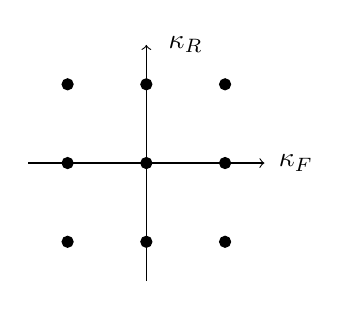
\begin{tikzpicture}
\draw[->] (-1.5,0) -- (1.5,0);
\draw[->] (0,-1.5) -- (0,1.5);
\filldraw[black] (0,0) circle (2pt);
\filldraw[black] (-1,0) circle (2pt);
\filldraw[black] (0,-1) circle (2pt);
\filldraw[black] (1,0) circle (2pt);
\filldraw[black] (0,1) circle (2pt);
\filldraw[black] (-1,-1) circle (2pt);
\filldraw[black] (1,-1) circle (2pt);
\filldraw[black] (-1,1) circle (2pt);
\filldraw[black] (1,1) circle (2pt);
\node at (0.5,1.5) {$\kappa_R$};
\node at (1.9,0) {$\kappa_F$};
\end{tikzpicture}}
\begin{caption}{Symmetric prescriptions for a single process, indicating
    the sampled values for the factorisation scale $\kappa_F$ and 
    renormalisation scale $\kappa_R$ in each case.
    %
    The origin of coordinates corresponds to the
    central scales $\kappa_F=\kappa_R= 0$.
    %
    We show the three prescriptions 
    $5$-point (left), $\bar{5}$-point (middle) and $9$-point (right).
\label{fig:symmetricPrescriptions}
  }
\end{caption}
\end{figure}
%%%%%%%%%%%%%%%%%%%%%%%%%%%%%%%%%%%%%%%%%%%%%%%%%%%%%%%%%%%%%%%%%%%%%%%%%%%%%%%
\begin{itemize}
\item \textbf{5-point}: 
$v_4 = \{(\pm;0), (0; \pm) \}$ and $n_4 = 2/4 = 1/2$. This amounts to scale variation for each scale in turn, keeping the other fixed. We find the covariance matrix
\be \label{5S}
    S^{\rm (5pt)}_{ij} = \smallfrac{1}{2}\big\{ \Delta_i^{+0}\Delta_j^{+0} + \Delta_i^{-0} \Delta_j^{-0} + \Delta_i^{0+} \Delta_j^{0+} + \Delta_i^{0-} \Delta_j^{0-}  \big\} \, .
\ee
We find that the variations of each scale are added together in quadrature, as one would expect for independent contributions to the MHOU.
\item \textbf{$\overline{5}$-point}:
$\overline{v}_4 = \{(\pm; \pm) \}$, where $(\pm;\pm)$ are assumed
  uncorrelated, and $\overline{n}_4 = 2/4 = 1/2$. This is the complement of 5-point, exploring a different region of scale variation space.
\be
 \label{5bS}
    S^{(\rm \overline{5}pt)}_{ij} = \smallfrac{1}{2}\big\{ \Delta_i^{++}\Delta_j^{++} + \Delta_i^{--}\Delta_j^{--} + \Delta_i^{+-}\Delta_j^{+-} + \Delta_i^{-+} \Delta_j^{-+}\big\} \, .
\ee
\item \textbf{9-point}: $v_8=v_4\oplus \overline{v}_4$ (the union of 5-point and
  $\overline{5}$-point) and $n_8 = 2/8 = 1/4$. Here we include every combination, varying the scales totally independently. 
\be \label{9S}
\begin{split}
    S^{(\rm 9pt)}_{ij} = \smallfrac{1}{4}\big\{ &\Delta_i^{+0} \Delta_j^{+0} + \Delta_i^{-0}\Delta_j^{-0}
                            + \Delta_i^{0+} \Delta_j^{0+} + \Delta_i^{0-}\Delta_j^{0-} \\
                            + &\Delta_i^{++}\Delta_j^{++} + \Delta_i^{+-} \Delta_j^{+-}
                            + \Delta_i^{-+}\Delta_j^{-+} + \Delta_i^{--} \Delta_j^{--} \big\} \, .
\end{split}                            
\ee 
\end{itemize}
\subsubsection{Two processes}
In the case that $p=2$ we can have either uncorrelated or partially correlated scale variations. We will have $p+1=3$ independent scales to vary, and our set of scale variation points, $V_m$, will be much larger than for one process ($v_m$). If we label the processes $a=1, b=2$, we can view the two-process covariance matrix as
\be  
  S_{ij} = \left(\begin{array}{cc}
S_{i_1j_1}&S_{i_1j_2}\\ 
S_{i_2j_1}&S_{i_2j_2}\end{array}\right)\, ,
\ee
so the diagonal elements deal with data points in the same process, and the off-diagonals deal with data points in different processes. For the diagonal blocks, the form of $S$ must be equivalent to the $p=1$ case, and so 
\be
S_{i_1j_1}= N_m \sum_{V_m} \Delta_{i_1} (\kappa_F, \kappa_{R_1}) \Delta_{j_1} (\kappa_F, \kappa_{R_1})=
n_{m} \sum_{v_{m}} \Delta_{i_1} (\kappa_F, \kappa_{R_1})\Delta_{j_1} (\kappa_F, \kappa_{R_1}) \, .
\ee
This means that $v_m$ must be a subset of $V_m$, so that if we sum over $V_m$ setting $\kappa_{R_2}$ to 0, we should recover $v_m$ up to a degeneracy factor, $d_m$, which is the number of copies of $v_m$ in $V_m$. This means the overall normalisation factor is
\be 
N_m = n_m/d_m \, .
\ee
We now go on to consider the 5-point, $\overline{5}$-point and 9-point prescriptions for the case of two processes, depicted in Fig.~\ref{fig:symmetricPrescriptions2proc}. We expand the notation to include three scales, that is $(\kappa_F; \kappa_{R_1},\kappa_{R_2})$.
%%%%%%%%%%%%%%%%%%%%%%%%%%%%%%%%%%%%%%%%%%%%%%%%%%%%%%%%%%%%%5
\begin{figure}[t]
\centering
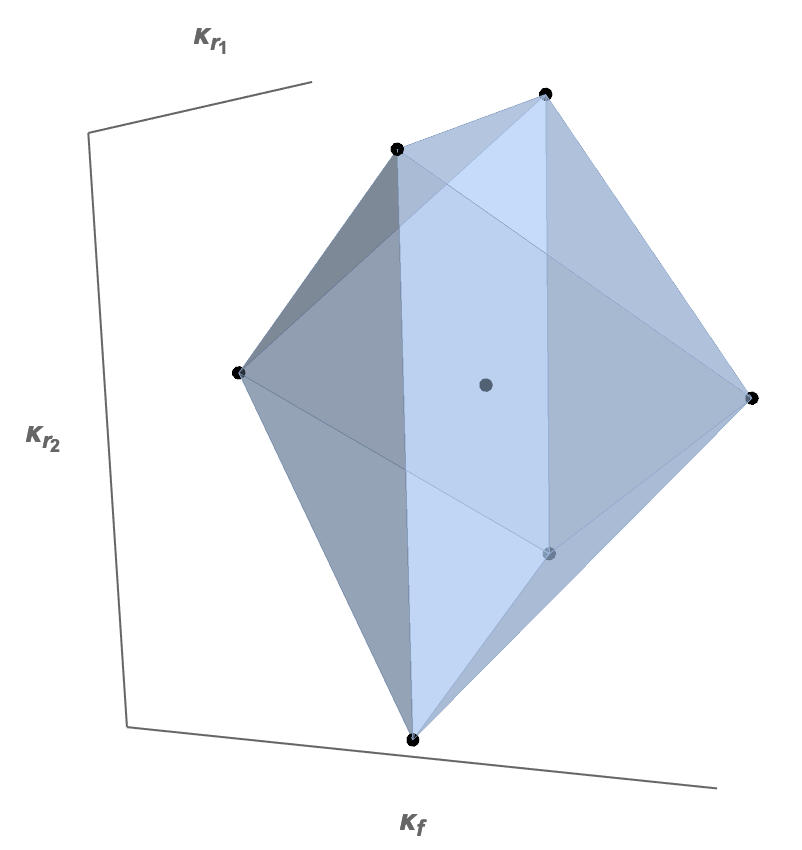
\includegraphics[scale=0.35]{mhous/plots/5pt_3D.png}
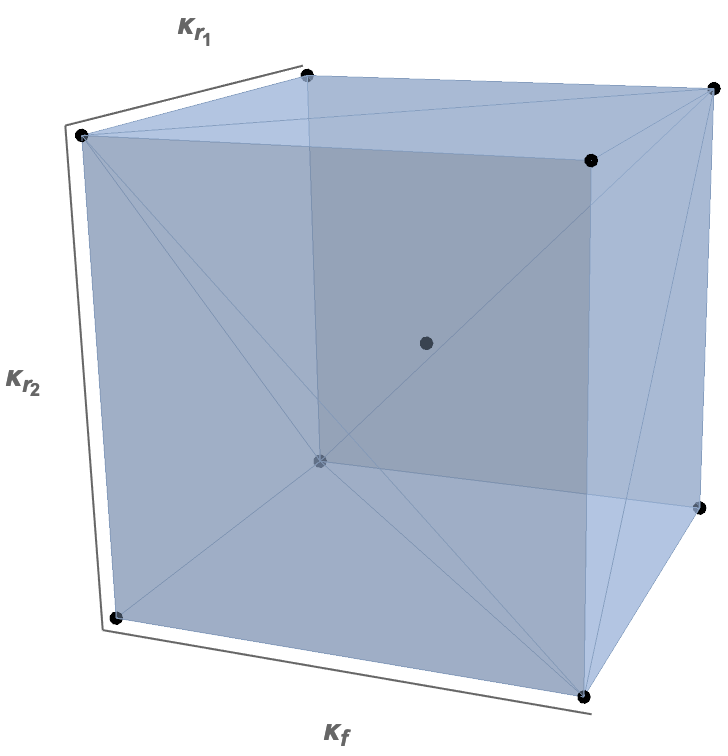
\includegraphics[scale=0.35]{mhous/plots/5barpt_3D.png}
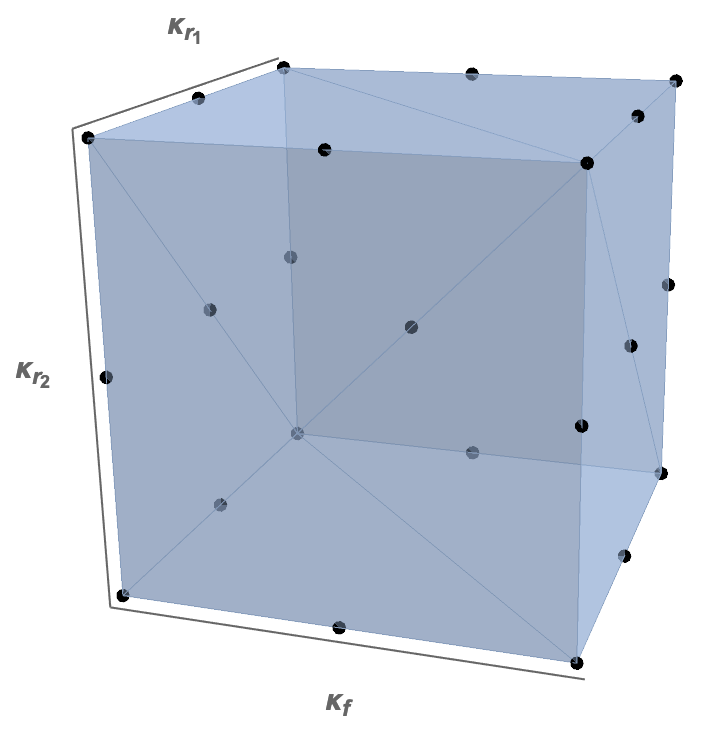
\includegraphics[scale=0.35]{mhous/plots/9pt_3D.png}
\begin{caption}{\small Same as Fig.~\ref{fig:symmetricPrescriptions}, now
    for the case of two different processes with a common factorisation scale, $\kappa_F,$ and different renormalisation scales, $\kappa_{R_1}$
    and $\kappa_{R_2}$, so the diagrams are now in 3d.
    %
    We again show the three prescriptions $5$-point (left), $\bar{5}$-point (middle) and $9$-point (right).}
  \label{fig:symmetricPrescriptions2proc}
\end{caption}
\end{figure}
%%%%%%%%%%%%%%%%%%%%%%%%%%%%%%%%%%%%%%%%%%%%%%%%%%%%%%%%%%%
\begin{itemize}
\item \textbf{5-point}: 
We vary the factorisation scale holding the renormalisation scales fixed,  and the renormalisation scales holding the factorisation scale fixed, so that
$V_4 = \{2(\pm;0,0), (0;\pm,\pm)\}$. This means $V_4$
  has eight elements in total. The factor of two comes from considering the one-process case, where we can set $\kappa_{R_2}=0$, and must return a multiple of $v_4$. Explicitly, we will get $\{2(\pm;0,0), 2(0;\pm,0)\}$, picking up a factor of two on the second term because there are two terms implicitly here, for $\kappa_{R_2}$ = $+$ and $-$. We need to include a factor of two from the outset on the first term so we end up with an overall factor at the end, in this case $d_4 =2$. This means $N_4 = (1/2)/2 = 1/4$. The off-diagonal blocks of the covariance matrix are evaluated as
 \be \label{eqn:5ptmult}
     S^{(\rm 5pt)}_{i_1j_2} = \smallfrac{1}{4}\big\{ 2\Delta_{i_1}^{+0}\Delta_{j_2}^{+0} + 2\Delta_{i_1}^{-0}\Delta_{j_2}^{-0}  
            + \big(\Delta_{i_1}^{0+} + \Delta_{i_1}^{0-} \big)\big(\Delta_{j_2}^{0+} + \Delta_{j_2}^{0-}\big)\big\}.
 \ee
When generalising to 3 processes, we simply write $V_4 = \{4(\pm;0,0,0)$, $(0;\pm,\pm, \pm)\}$, and this time $d_4=4$ by the same arguments as above. However, we can still use Eqn.~\ref{eqn:5ptmult} to evalutate all of the off-diagonal blocks because we will only ever be considering two of the three processes at a time. 
\item \textbf{$\overline{5}$-point}:
$\overline{V}_4 = \{(\pm;\pm,\pm)\}$, so we are essentially exploring the outer corners of the 3d scale variation space. $\overline{V}_4$ has eight elements, and there are two elements for each in $\overline{v}_4$, meaning that $\overline{N}_4 = (1/2)/2 = 1/4$. The off-diagonal blocks of the covariance matrix are evaluated as
\be 
    S^{(\rm \overline{5}pt)}_{i_1j_2} = \smallfrac{1}{4}\big\{ \big(\Delta_{i_1}^{++} + \Delta_{i_1}^{+-}\big) \big(\Delta_{j_2}^{++} + \Delta_{j_2}^{+-} \big) 
    + \big(\Delta_{i_1}^{-+} + \Delta_{i_1}^{--}\big) \big(\Delta_{j_2}^{-+} + \Delta_{j_2}^{--} \big) \big\} \, .
\ee
For three processes the generalisation is simply $\overline{V}_4 = \{(\pm;\pm,\pm,\pm)\}$, with $\overline{N}_4 = 1/8$. 
\item \textbf{9-point}: Again, all three scales are varied completely independently and $V_8= \{3(0;\pm,\pm), 2(\pm;\pmz,\pmz)\}$, where $\pmz$ means either $+$, $-$ or $0$. Note the factors of 2 and 3, which arise from arguments similar to that for 5-point; namely, that $V_8$ must reduce to a multiple of $v_8$ when $\kappa_{R_2}$ is set to 0. The overall $d_8$ = 6 and so $N_8 = 1/24$. The off-diagonal blocks of the covariance matrix are 
\begin{equation}
\begin{split}
    S^{(\rm 9pt)}_{i_1j_2} =
    \smallfrac{1}{24}\big\{&2\big(\Delta_{i_1}^{+0}+\Delta_{i_1}^{++}
    + \Delta_{i_1}^{+-}\big) \big(\Delta_{j_2}^{+0} +
    \Delta_{j_2}^{++} + \Delta_{j_2}^{+-} \big) \\ 
            + &2\big(\Delta_{i_1}^{-0} + \Delta_{i_1}^{-+} +
            \Delta_{i_1}^{--}\big)\big(\Delta_{j_2}^{-0} +
            \Delta_{j_2}^{-+} + \Delta_{j_2}^{--} \big) \big\}\\ 
            + &3\big(\Delta_{i_1}^{0+}+ \Delta_{i_1}^{0-}\big)\big(\Delta_{j_2}^{0+} + \Delta_{j_2}^{0-} \big)\big\}.
\end{split}            
\end{equation}
For three processes, $V_8= \{9(0;\pm,\pm,\pm),
4(\pm;\pmz,\pmz,\pmz)\}$ and $d_8=36$.
\end{itemize}
\subsection{Asymmetric prescriptions}
It is sometimes argued that since only the cross-section is actually physical, a single process has only one scale, namely the ``scale of the process". This is like setting $\kappa_F = \kappa_R$. In addition, it is also possible to consider varying the scale of the process on top of the variation of factorisation and renormalisation scales already considered. The logic behind this is that the three scales each estimate a different source of MHOU:
\begin{itemize}
\item Varying the scale of the process estimates the MHOU on the hard cross section which is proportional to collinear logarithms;
\item Varying the renormalisation scale estimates the MHOU on the hard cross section which is proportional to the beta function;
\item Varying the factorisation scale estimates the MHOU in the anomalous dimension.
\end{itemize}
However, both of these approaches will suppress correlations between uncertainties in PDF evolution across different processes, and may therefore overestimate the MHOU. Ultimately, the best scheme, be it a symmetric or an asymmetric prescription, must be established through a validation procedure such as the one outlined in later sections.

We will now formulate prescriptions for these two asymmetric prescriptions, being the 3-point and 7-point prescriptions, respectively. These are depicted for a single process in Fig.~\ref{fig:AsymmetricPrescriptions1proc}.
%%%%%%%%%%%%%%%%%%%%%%%%%%%%%%%%%%%%%%%%%%%%%%%%%%%%%%%%%%%%%%%%%%%%%%%%%%%%%%%%%%%%%%%%%%%
\begin{figure}[t]
\centering
{\begin{tikzpicture}
\draw[->] (-1.5,0) -- (1.5,0);
\draw[->] (0,-1.5) -- (0,1.5);
\filldraw[black] (0,0) circle (2pt);
\filldraw[black] (-1,-1) circle (2pt);
\filldraw[black] (1,1) circle (2pt);
\node at (0.5,1.5) {$\kappa_R$};
\node at (1.9,0) {$\kappa_F$};
\end{tikzpicture}}\qquad
{\begin{tikzpicture}
\draw[->] (-1.5,0) -- (1.5,0);
\draw[->] (0,-1.5) -- (0,1.5);
\filldraw[black] (0,0) circle (2pt);
\filldraw[black] (-1,0) circle (2pt);
\filldraw[black] (0,-1) circle (2pt);
\filldraw[black] (1,0) circle (2pt);
\filldraw[black] (0,1) circle (2pt);
\filldraw[black] (-1,-1) circle (2pt);
\filldraw[black] (1,1) circle (2pt);
\node at (0.5,1.5) {$\kappa_R$};
\node at (1.9,0) {$\kappa_F$};
\end{tikzpicture}}
\begin{caption}{Same as Fig.~\ref{fig:symmetricPrescriptions},
    now in the case of the asymmetric prescriptions for a single process
    with factorisation scale $\kappa_F$ and renormalisation scale $\kappa_R$.
    %
    We display the 
    $3$-point (left) and $7$-point (right) prescriptions, defined in the text.}
  \label{fig:AsymmetricPrescriptions1proc}
\end{caption}
\end{figure}
%%%%%%%%%%%%%%%%%%%%%%%%%%%%%%%%%%%%%%%%%%%%%%%%%%%%%%%%%%%%%%%%%%%%%%%%%%%%%%%%%%%%%%%%%%%
\begin{itemize}
\item \textbf{3-point}: We set $\kappa_F=\kappa_R$ and vary this scale. We have $v_2 = \{\pm\}$ and $s =1$, $m=2$ and $n_2 = 1/2$, so we are just averaging over the two scale-varied options. For a single process
\be 
   S^{(\rm 3pt)}_{ij} = \smallfrac{1}{2}\big\{ \Delta_i^{++}\Delta_j^{++}  + \Delta_i^{--}\Delta_j^{--}\big\} \, .
\ee
For two different processes we have $V_2 = \{\pm, \pm\}$, and can see explicitly that we are ignoring the correlations in $\kappa_F$ between the two processes. We have $d_2 =2$ and so $N_2 = (1/2)/2 =1/4$, and the off-diagonal blocks of the covariance matrix are evaluated as
\be 
    S^{(\rm 3pt)}_{i_1j_2} = \smallfrac{1}{4}\big\{\big(\Delta_{i_1}^{++} + \Delta_{i_1}^{--} \big) \big(\Delta_{j_2}^{++} + \Delta_{j_2}^{--} \big) \big\}\, .
\ee
\item \textbf{7-point}: We combine varying the scale of the process with $\kappa_R$ and $\kappa_F$ variation. We will end up with essentially a combination of 3-point (scale of process) and 5-point (individual factorisation and renormalisation). For a single process, $v_6 = \{(\pm;0),(0;\pm),(+;+),(-;-)\} =\{(\pm;0),(0;\pm),(\overline{\pm;\pm})\}$, where $(\overline{\pm;\pm})$ simply means that the variation is fully correlated (so there are only 2 terms, not 4). Then $s=2$ and $m=6$ so $n_6 =1/3$, and for a single process
\be
 S^{(\rm 7pt)}_{ij} = \smallfrac{1}{3}\big\{ \Delta_i^{+0}\Delta_j^{+0} + \Delta_i^{-0}\Delta_j^{-0} + \Delta_i^{0+}\Delta_j^{0+}  + \Delta_i^{0-}\Delta_j^{0-}  
        + \Delta_i^{++}\Delta_j^{++} + \Delta_i^{--}\Delta_j^{--}  \big\} \, .
\ee
For more than one process, variations of the scale of the process are uncorrelated between processes so the $\mu_F$ variation enclosed in the scale of the process variation will be decorrelated. So overall for two processes we will be in a 4d scale variation space, 
$(\kappa_{F_1},\kappa_{R_1};\kappa_{F_2},\kappa_{R_2})$. Then $V_6=\{2(+,0;+,0),2(-,0;-,0),(0,\pm;0,\pm),(\overline{\pm,\pm};\overline{\pm,\pm})\}$, where $(\overline{\pm,\pm};\overline{\pm,\pm})=\{(+,+;+,+),(+,+;-,-),(-,-;+,+),(-,-;-,-)\}$, and thus $d_6=2$, so $N_6=1/6$, and the off-diagonal theory covariance matrix reads
\be 
  \begin{split}
    S^{(\rm 7pt)}_{i_1j_2} =& \smallfrac{1}{6}\big\{ 2\Delta_{i_1}^{+0} \Delta_{j_2}^{+0}  + 2\Delta_{i_1}^{-0} \Delta_{j_2}^{-0} 
             + \big(\Delta_{i_1}^{0+}+\Delta_{i_1}^{0-}\big)\big(\Delta_{j_2}^{0+} + \Delta_{j_2}^{0-} \big)
            \\&+\big(\Delta_{i_1}^{++}+\Delta_{i_1}^{--}\big) \big(\Delta_{j_2}^{++} + \Delta_{j_2}^{--} \big) \big\} \, .
            \end{split}
\ee
\end{itemize}

\section{Results for the theory covariance matrix}
\label{sec:results}
In this section we summarise the data used to calculate theory covariance matrices using the prescriptions in the previous section. We divide the data into processes, each with a distinct renormalisation scale. We present the theory covariance matrices for each prescription at NLO.

\subsection{Input data and process categorisation}
In order to use these prescriptions, we must first divide our data into distinct ``processes". There is some degree of arbitrariness here, but the idea is to group together data which might have a similar structure of MHOUs under a common renormalisation scale. First we will review the data included in these fits, then we will outline the process categorisation. This is summarised in Table~\ref{tab:datasets_process_categorisation}.

The data considered here are a mildly altered version of those in NNPDF3.1~\cite{Ball:2017nwa}. More exactly, they include: fixed-target~\cite{Arneodo:1996kd,Arneodo:1996qe,
Whitlow:1991uw,bcdms1,bcdms2,Goncharov:2001qe,MasonPhD,Onengut:2005kv} 
and HERA~\cite{Abramowicz:2015mha} DIS structure functions;
charm cross-sections from HERA~\cite{Abramowicz:1900rp};
gauge boson production from the Tevatron~\cite{Aaltonen:2010zza,Abazov:2007jy,
D0:2014kma,Abazov:2013rja}; electroweak boson production, 
inclusive jet, $Z$ $p_T$ distributions, and $t\bar{t}$ total and differential
cross-sections from ATLAS~\cite{Aad:2011dm,Aaboud:2016btc,Aad:2014qja,
Aad:2013iua,Aad:2015auj,Aad:2011fc,Aad:2014kva,Aaboud:2016pbd,Aad:2015mbv},
CMS~\cite{Chatrchyan:2013tia,Chatrchyan:2012xt,Chatrchyan:2013mza,
Khachatryan:2016pev,Khachatryan:2015oaa,Chatrchyan:2012bja,Khachatryan:2016mqs, 
Khachatryan:2015uqb,Khachatryan:2015oqa} 
and LHCb~\cite{Aaij:2012vn,Aaij:2012mda,Aaij:2015gna,Aaij:2015zlq}. In total they make up 2819 data points.
%%%%%%%%%%%%%%%%%%%%%%%%%%%%%%%%%%%%%%%%%%%%%%%%%%%%%%%%%
  %%%%%%%%%%%%%%%%%%%%%%%%%%%%%%%%%%%%%%%%%%%%%%%%%%%%%%%
\begin{center}
  \renewcommand*{\arraystretch}{1.50}
  \small
\begin{tabular}{|c|l|c|c|c|}
\toprule
  Process Type & Dataset   &  Reference    &  $N_{\rm dat}$     & $N_{\rm dat}$ (total)      \\
\midrule
\multirow{5}{*}{DIS NC}  & NMC    &  \cite{Arneodo:1996kd,Arneodo:1996qe}  & 134  &
\multirow{5}{*}{1593} \\
        & SLAC     & \cite{Whitlow:1991uw}     & 12  &    \\
        & BCDMS   & \cite{bcdms1,bcdms2}      & 530  & \\
        & HERA $\sigma^p_{NC}$     & \cite{Abramowicz:2015mha} & 886  & \\
        & HERA $\sigma^c_{NC}$     & \cite{Abramowicz:1900rp}  & 31  & \\
\midrule
\multirow{3}{*}{DIS CC}  & NuTeV dimuon  &\cite{Goncharov:2001qe,MasonPhD}
& 41  &
\multirow{3}{*}{552}\\
         & CHORUS  & \cite{Onengut:2005kv} & 430  &\\
        & HERA $\sigma^p_{CC}$   & \cite{Abramowicz:2015mha}& 81  & \\
\midrule
\multirow{19}{*}{DY}      &
  ATLAS $W,Z$, 7 TeV 2010  & \cite{Aad:2011dm} & 30  & \multirow{19}{*}{484}  \\
& ATLAS $W,Z$, 7 TeV 2011  &  \cite{Aaboud:2016btc} & 34  & \\
& ATLAS low-mass DY 2011  & \cite{Aad:2014qja} & 4  &\\
& ATLAS high-mass DY 2011  & \cite{Aad:2013iua} & 5  &\\
& ATLAS $Z$ $p_T$ 8 TeV ($p_T^{ll}, M_{ll}$) & \cite{Aad:2015auj} & 44  &\\
& ATLAS $Z$ $p_T$ 8 TeV ($p_T^{ll}, y_Z$) & \cite{Aad:2015auj} &  48   &\\
& CMS Drell-Yan 2D 2011    &  \cite{Chatrchyan:2013tia}    & 88  &   \\
& CMS $W$ asy 840 pb   & \cite{Chatrchyan:2012xt}    & 11   &   \\
& CMS $W$ asy 4.7 pb       & \cite{Chatrchyan:2013mza}  &11   & \\
& CMS $W$ rap 8 TeV   &  \cite{Khachatryan:2016pev}     &  22  &     \\
& CMS $Z$ $p_T$ 8 TeV ($p_T^{ll},M_{ll}$)      &  \cite{Khachatryan:2015oaa}    & 28  &  \\
& LHCb $Z$ 940 pb      &  \cite{Aaij:2012vn}    & 9  &  \\
& LHCb $Z \to ee$ 2 fb   & \cite{Aaij:2012mda}    & 17  &      \\
& LHCb $W, Z \to \mu$ 7 TeV  &  \cite{Aaij:2015gna}    & 29  &   \\
& LHCb $W, Z \to \mu$ 8 TeV &  \cite{Aaij:2015zlq}     & 30  &      \\
& CDF $Z$ rap    &  \cite{Aaltonen:2010zza}       & 29   &     \\
& D0 $Z$ rap    &  \cite{Abazov:2007jy}        & 28  &     \\
& D0 $W\to e\nu$ asy  & \cite{D0:2014kma}         & 8  &     \\
& D0 $W\to\mu\nu$ asy     &  \cite{Abazov:2013rja}        &  9 &   \\
\midrule
\multirow{2}{*}{JET}   & ATLAS jets 2011 7 TeV    & \cite{Aad:2011fc}  &  31 &  \multirow{2}{*}{164}    \\
& CMS jets 7 TeV 2011       & \cite{Chatrchyan:2012bja}  &  133  &  \\
\midrule
\multirow{4}{*}{TOP}     &
ATLAS $\sigma_{tt}^{\rm top}$       & \cite{Aad:2014kva, Aaboud:2016pbd}  & 3  & \multirow{4}{*}{26}  \\
& ATLAS $t\bar{t}$ rap &  \cite{Aad:2015mbv} & 10   &\\
& CMS $\sigma_{tt}^{\rm top}$   & \cite{Khachatryan:2016mqs, Khachatryan:2015uqb}       &  3 &   \\
& CMS $t\bar{t}$ rap   & \cite{Khachatryan:2015oqa}& 10   &   \\
\bottomrule
Total    &         &        & 2819  &  2819  \\
\bottomrule
\end{tabular}
\end{center}
%%%%%%%%%%%%%%%%%%%%%%%%%%%%%%%%%%%%%%%%%%%%%%%%%%%%%%%%%%

%%%%%%%%%%%%%%%%%%%%%%%%%%%%%%%%%%%%%%%%%%%%%%%%%%%%%%%%%

We identify five categories to divide the data into: neutral current DIS (DIS NC); charged current DIS (DIS CC); Drell-Yan (DY); jet production (JET); and top production (TOP). These represent groups of data with similar expected MHO terms. For instance, predictions for DY processes can be differential in differing variables, but all are obtained by integrating the same underlying, fully differential, distribution. This means they should have a similar perturbative structure. On the other hand, these distributions constrain different PDFs and so complex correlations between the PDFs will be introduced. Note that DIS is split up into CC and NC due to the differing structure of interaction.

\subsection{NLO theory covariance matrices}
All calculations are performed using 
the same settings as in~\cite{Ball:2017nwa}. Theoretical predictions are provided by {\tt APFEL}~\cite{Bertone:2013vaa} for the DIS structure functions
and by {\tt APFELgrid}~\cite{Bertone:2016lga} combined with
{\tt APPLgrid}~\cite{Carli:2010rw} for the hadronic
cross-sections. They are all evaluated using the central NLO PDF obtained by performing a NLO fit to the same dataset, for consistency. The resulting predictions are then used to construct the theory covariance matrices using the {\tt ReportEngine} software~\cite{zahari_kassabov_2019_2571601}.

We now present the theory covariance matrices at NLO, and discuss their features. In Fig.~\ref{fig:diag_covmats} we compare the square root of the diagonal elements of the experiment ($C$) and theory ($S$) covariance matrices, normalised to experimental data values; these are equivalent to the fractional per-point uncertainties. In this and what follows, the data are grouped by process and, within each process, by dataset according to Table~\ref{tab:datasets_process_categorisation}, wherein they are binned according to kinematics (the same as in the experimental papers). $S$ is the 9-pt covariance matrix, being that with the largest number of independent scale variations. On the whole, the size of NLO MHOUs is comparable to the experimental uncertainties, and we can see that each will dominate in different regions. One particularly striking instance of this is seen in the HERA data, which can be found in the middle of DIS NC: for high ($x$, $Q^2$) there is low statistics and so the experimental uncertainties dominate; for low ($x$, $Q^2$) perturbation theory holds less strongly and the MHOUs dominate. 
%%%%%%%%%%%%%%%%%%%%%%%%%%%%%%%%%%%%%%%%%%%%%%%%%%%%%%%%%%%%%%%%%%%
\begin{figure}[t!]
  \begin{center}
    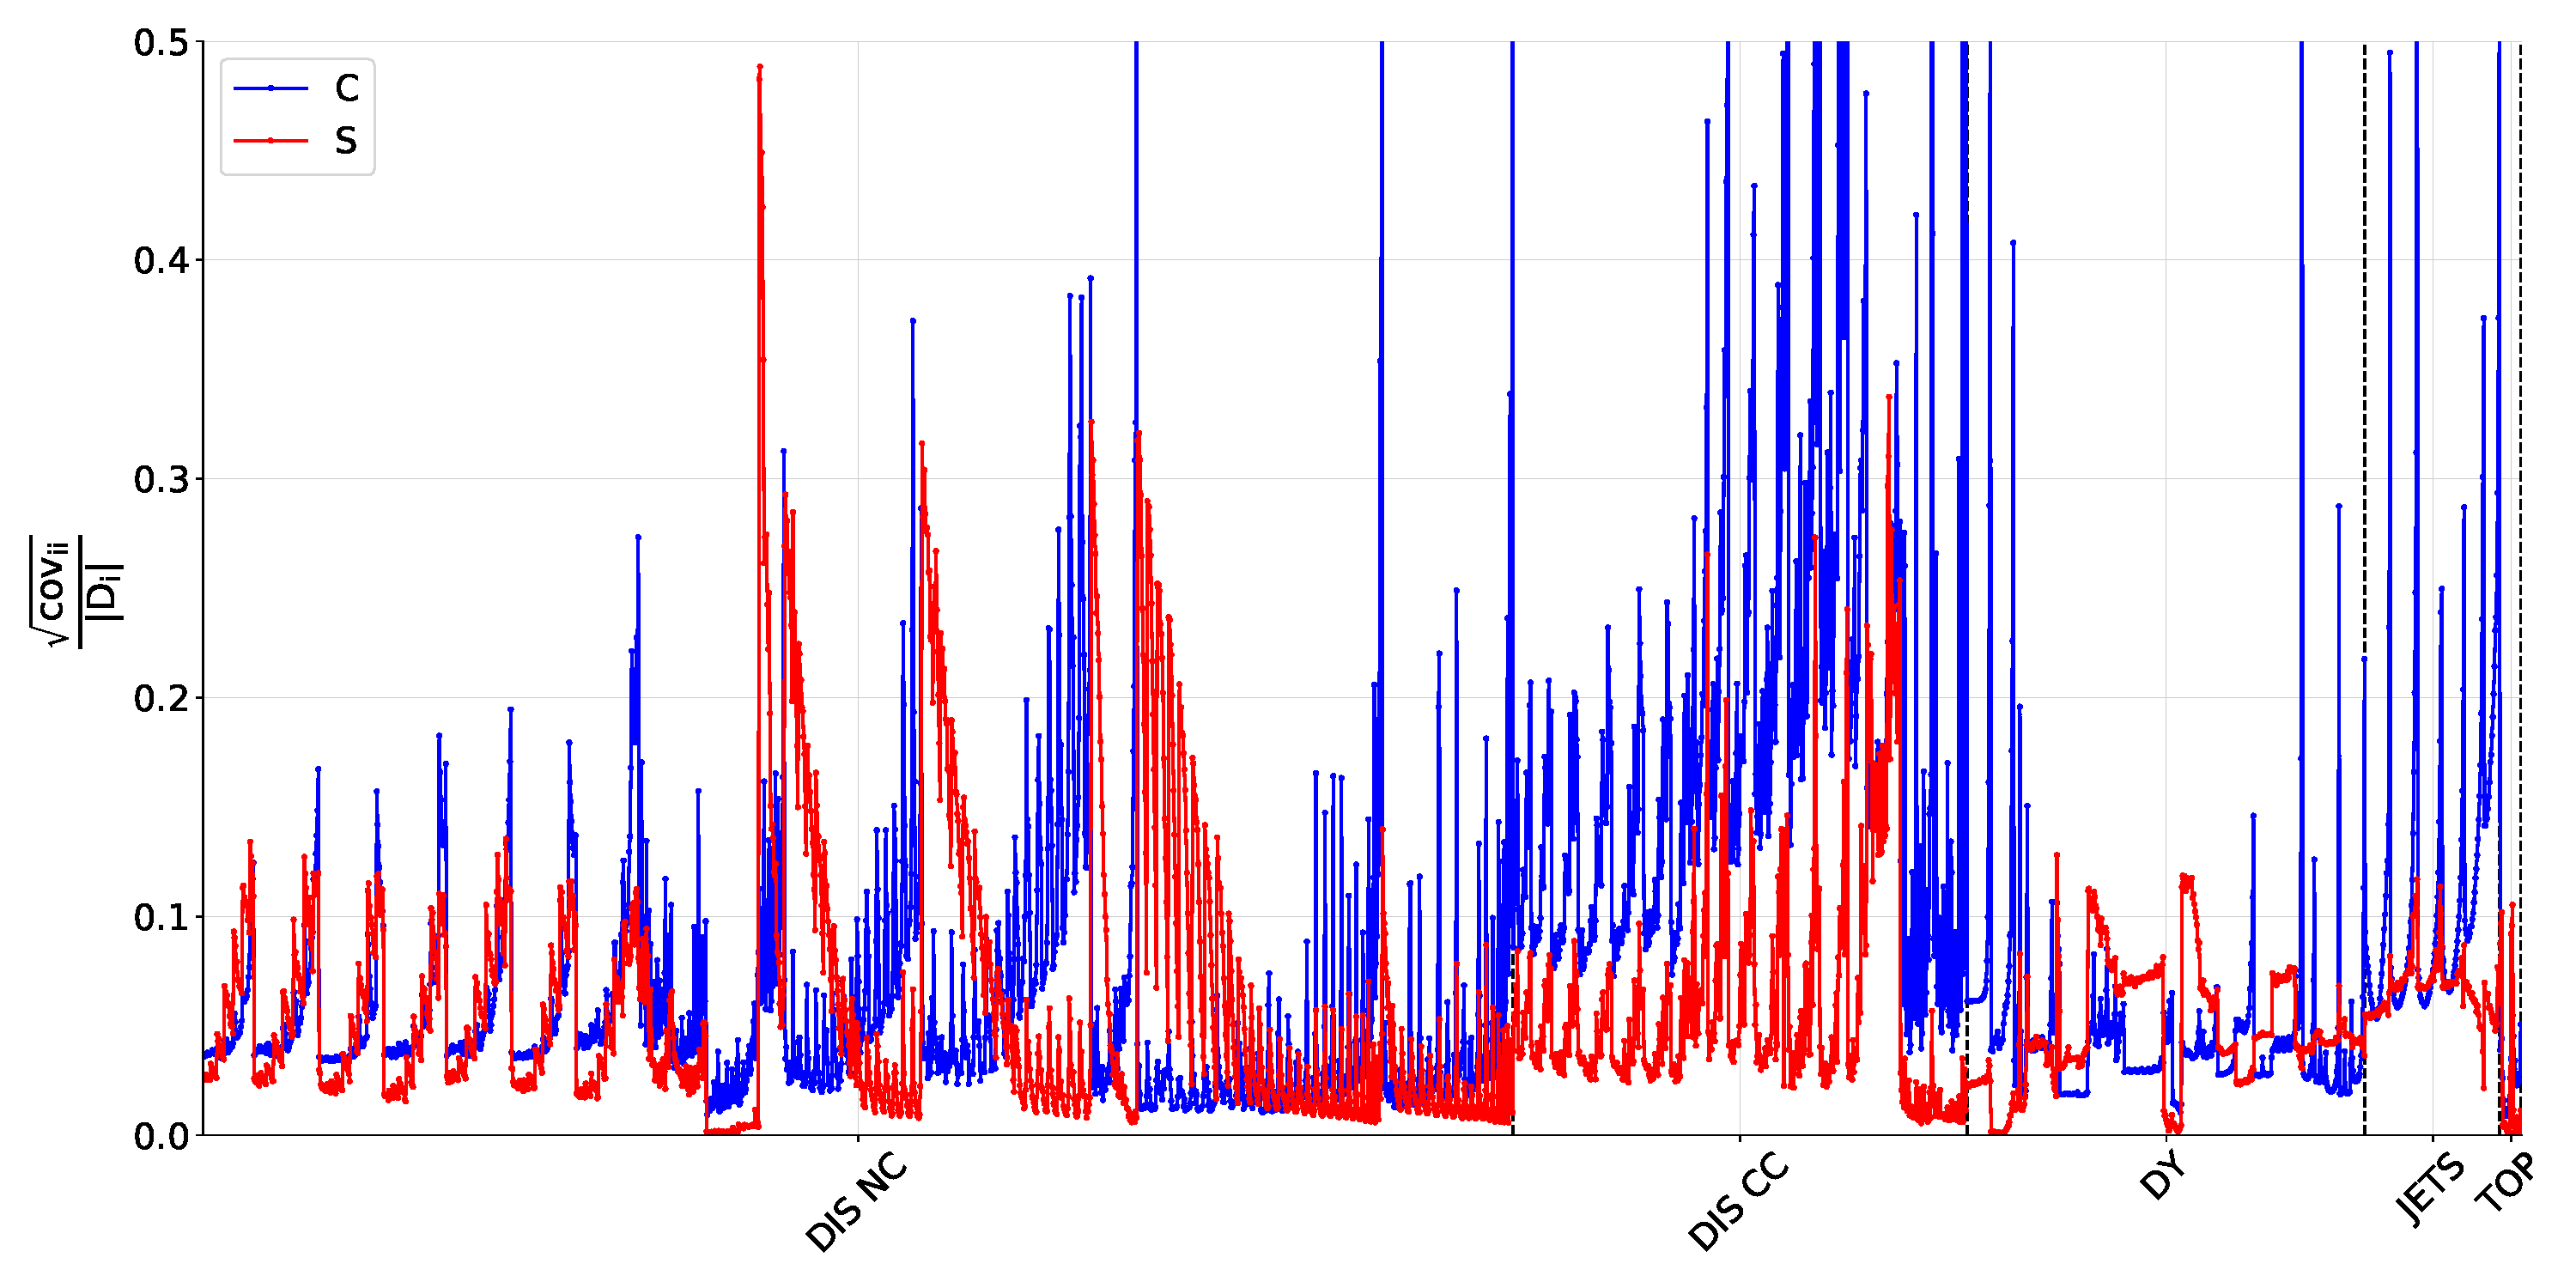
\includegraphics[width=1.0\linewidth]{mhous/plots/9pt_diagonal_elements.pdf}
    \caption{\small Comparison of the per-point experimental 
    (blue) and 9-point theoretical (red) uncertainties, normalised to data. In this and what follows, data are grouped by process and, within each process, by dataset, following
  Table~\ref{tab:datasets_process_categorisation} 
        \label{fig:diag_covmats} }
  \end{center}
%\end{figure}
%%%%%%%%%%%%%%%%%%%%%%%%%%%%%%%%%%%%%%%%%%%%%%%%%%%%%%%%%%%%%%%%%%%%%%
%%%%%%%%%%%%%%%%%%%%%%%%%%%%%%%%%%%%%%%%%%%%%%%%%%%%%%%%%%%%%%%%%%%
%\begin{figure}[t!]
  \begin{center}
    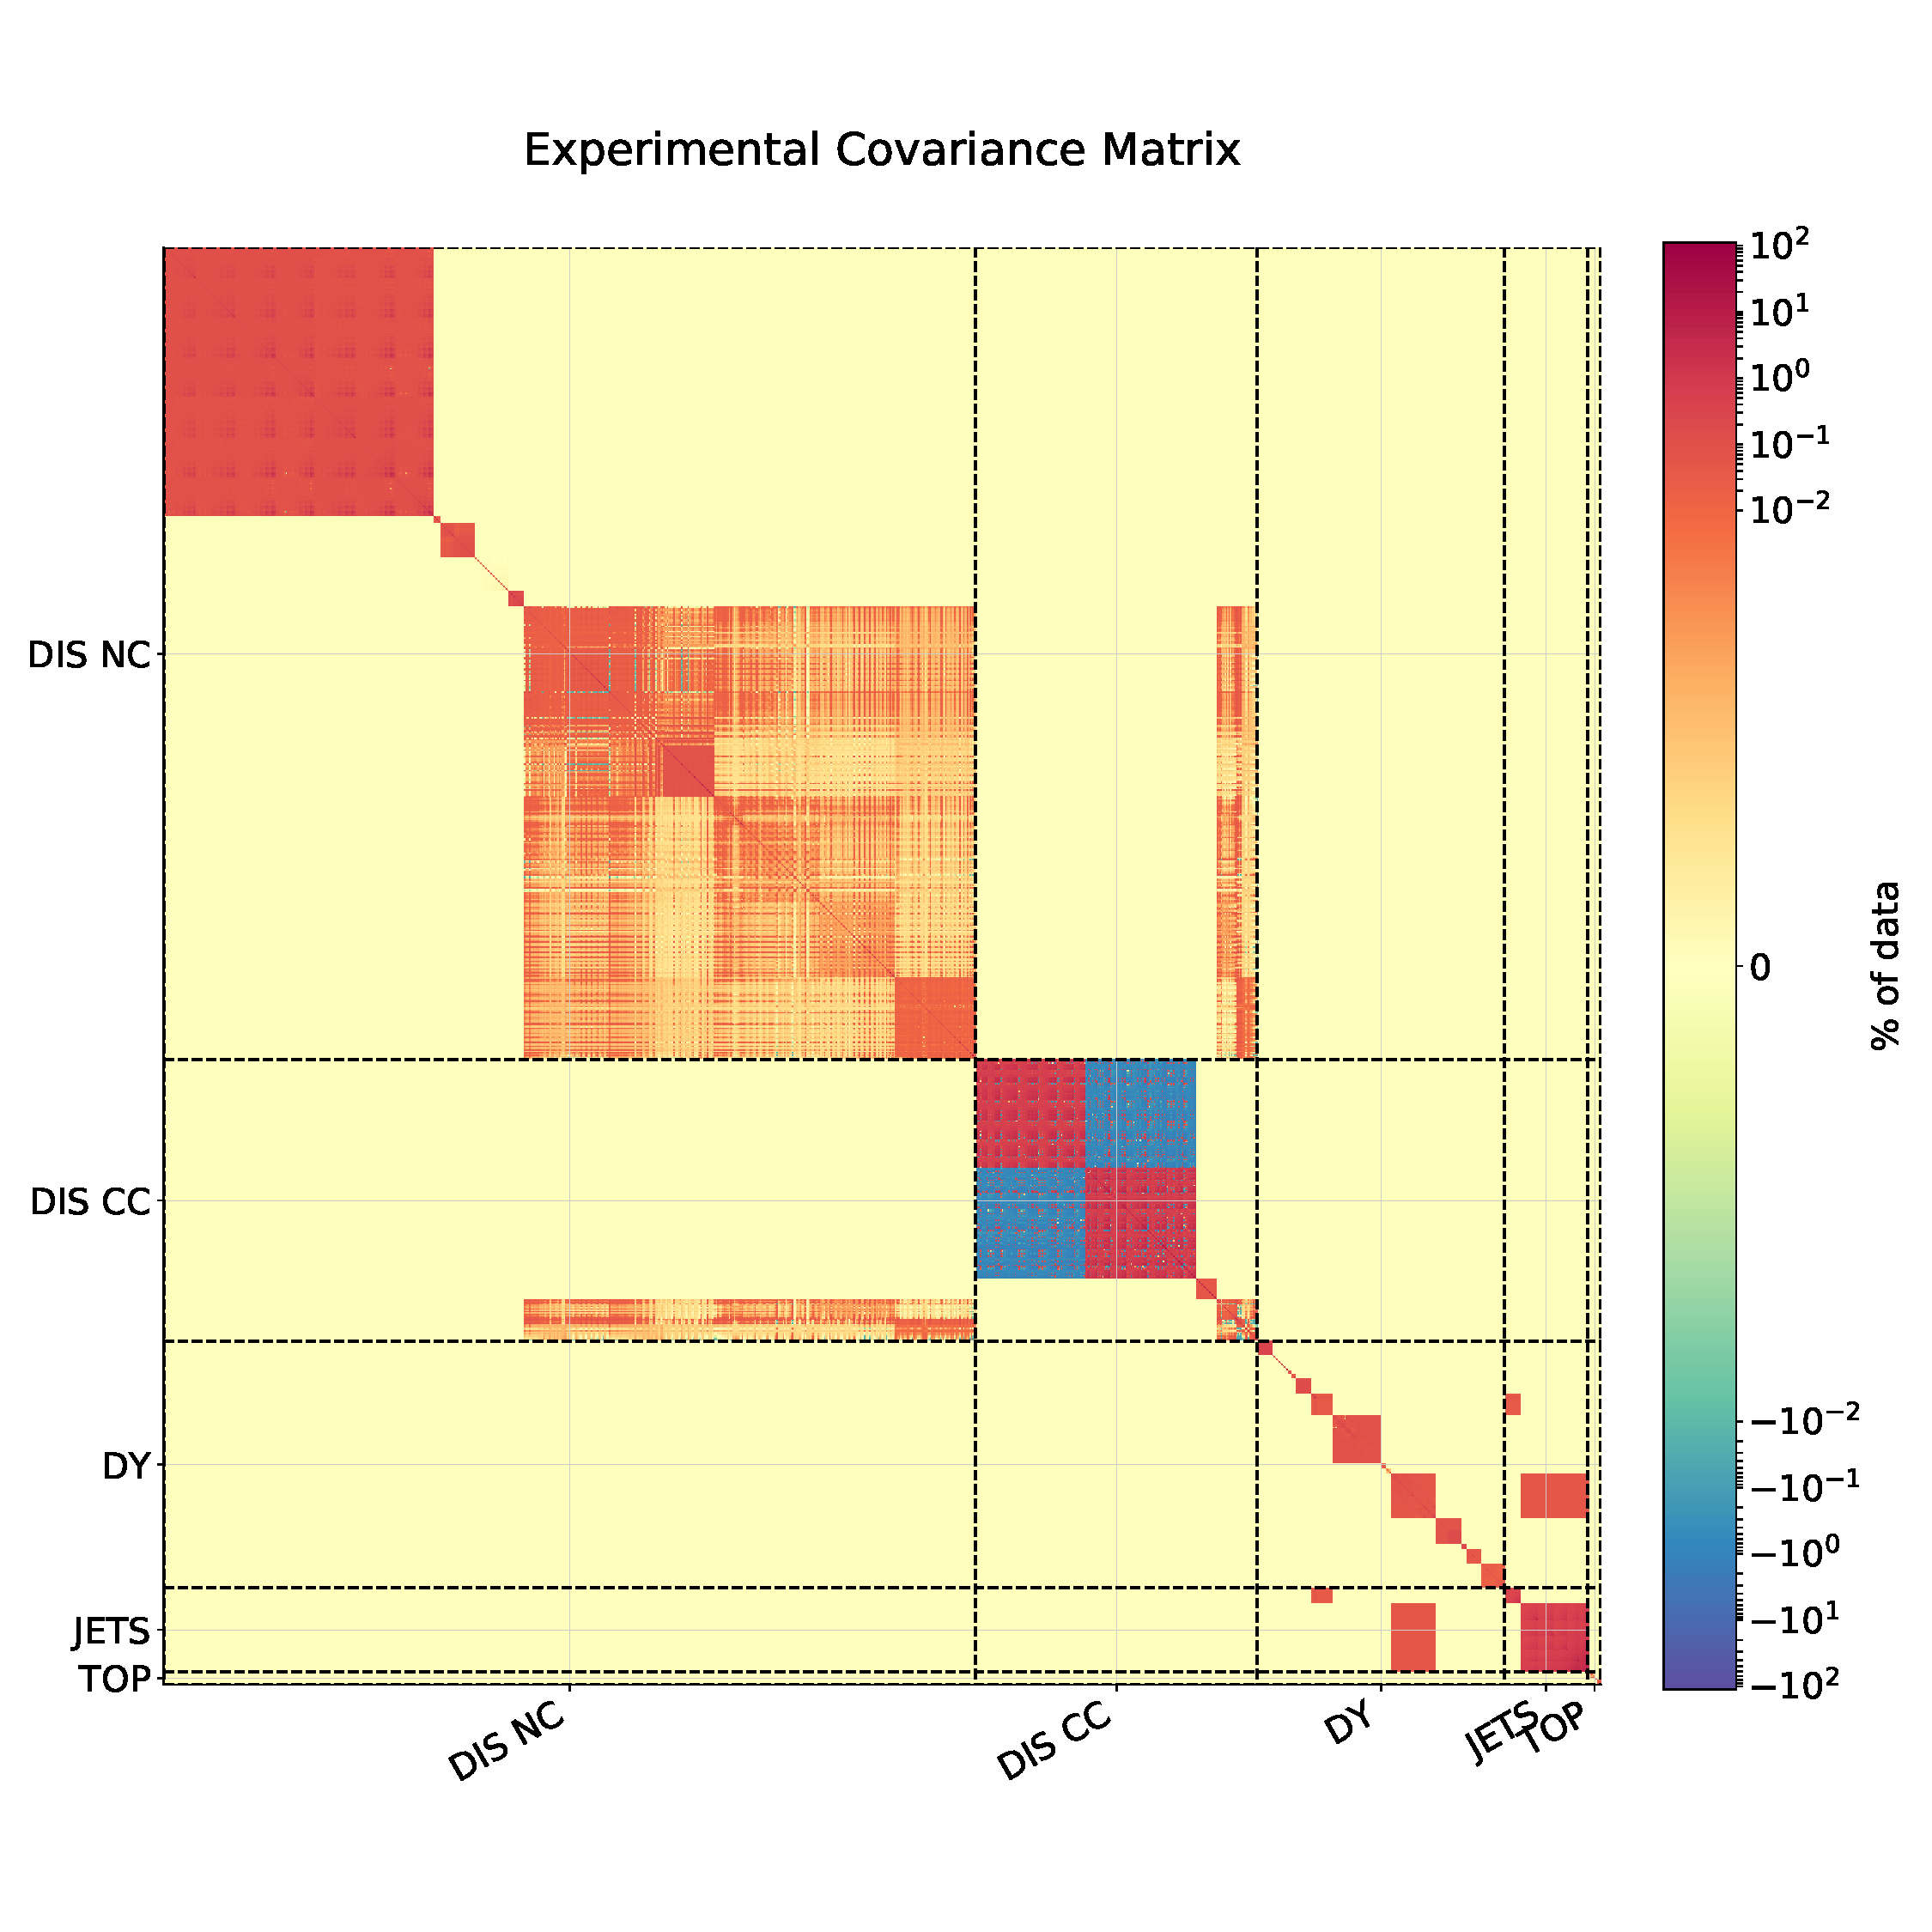
\includegraphics[width=0.49\linewidth]{mhous/plots/exp_covmat.pdf}
    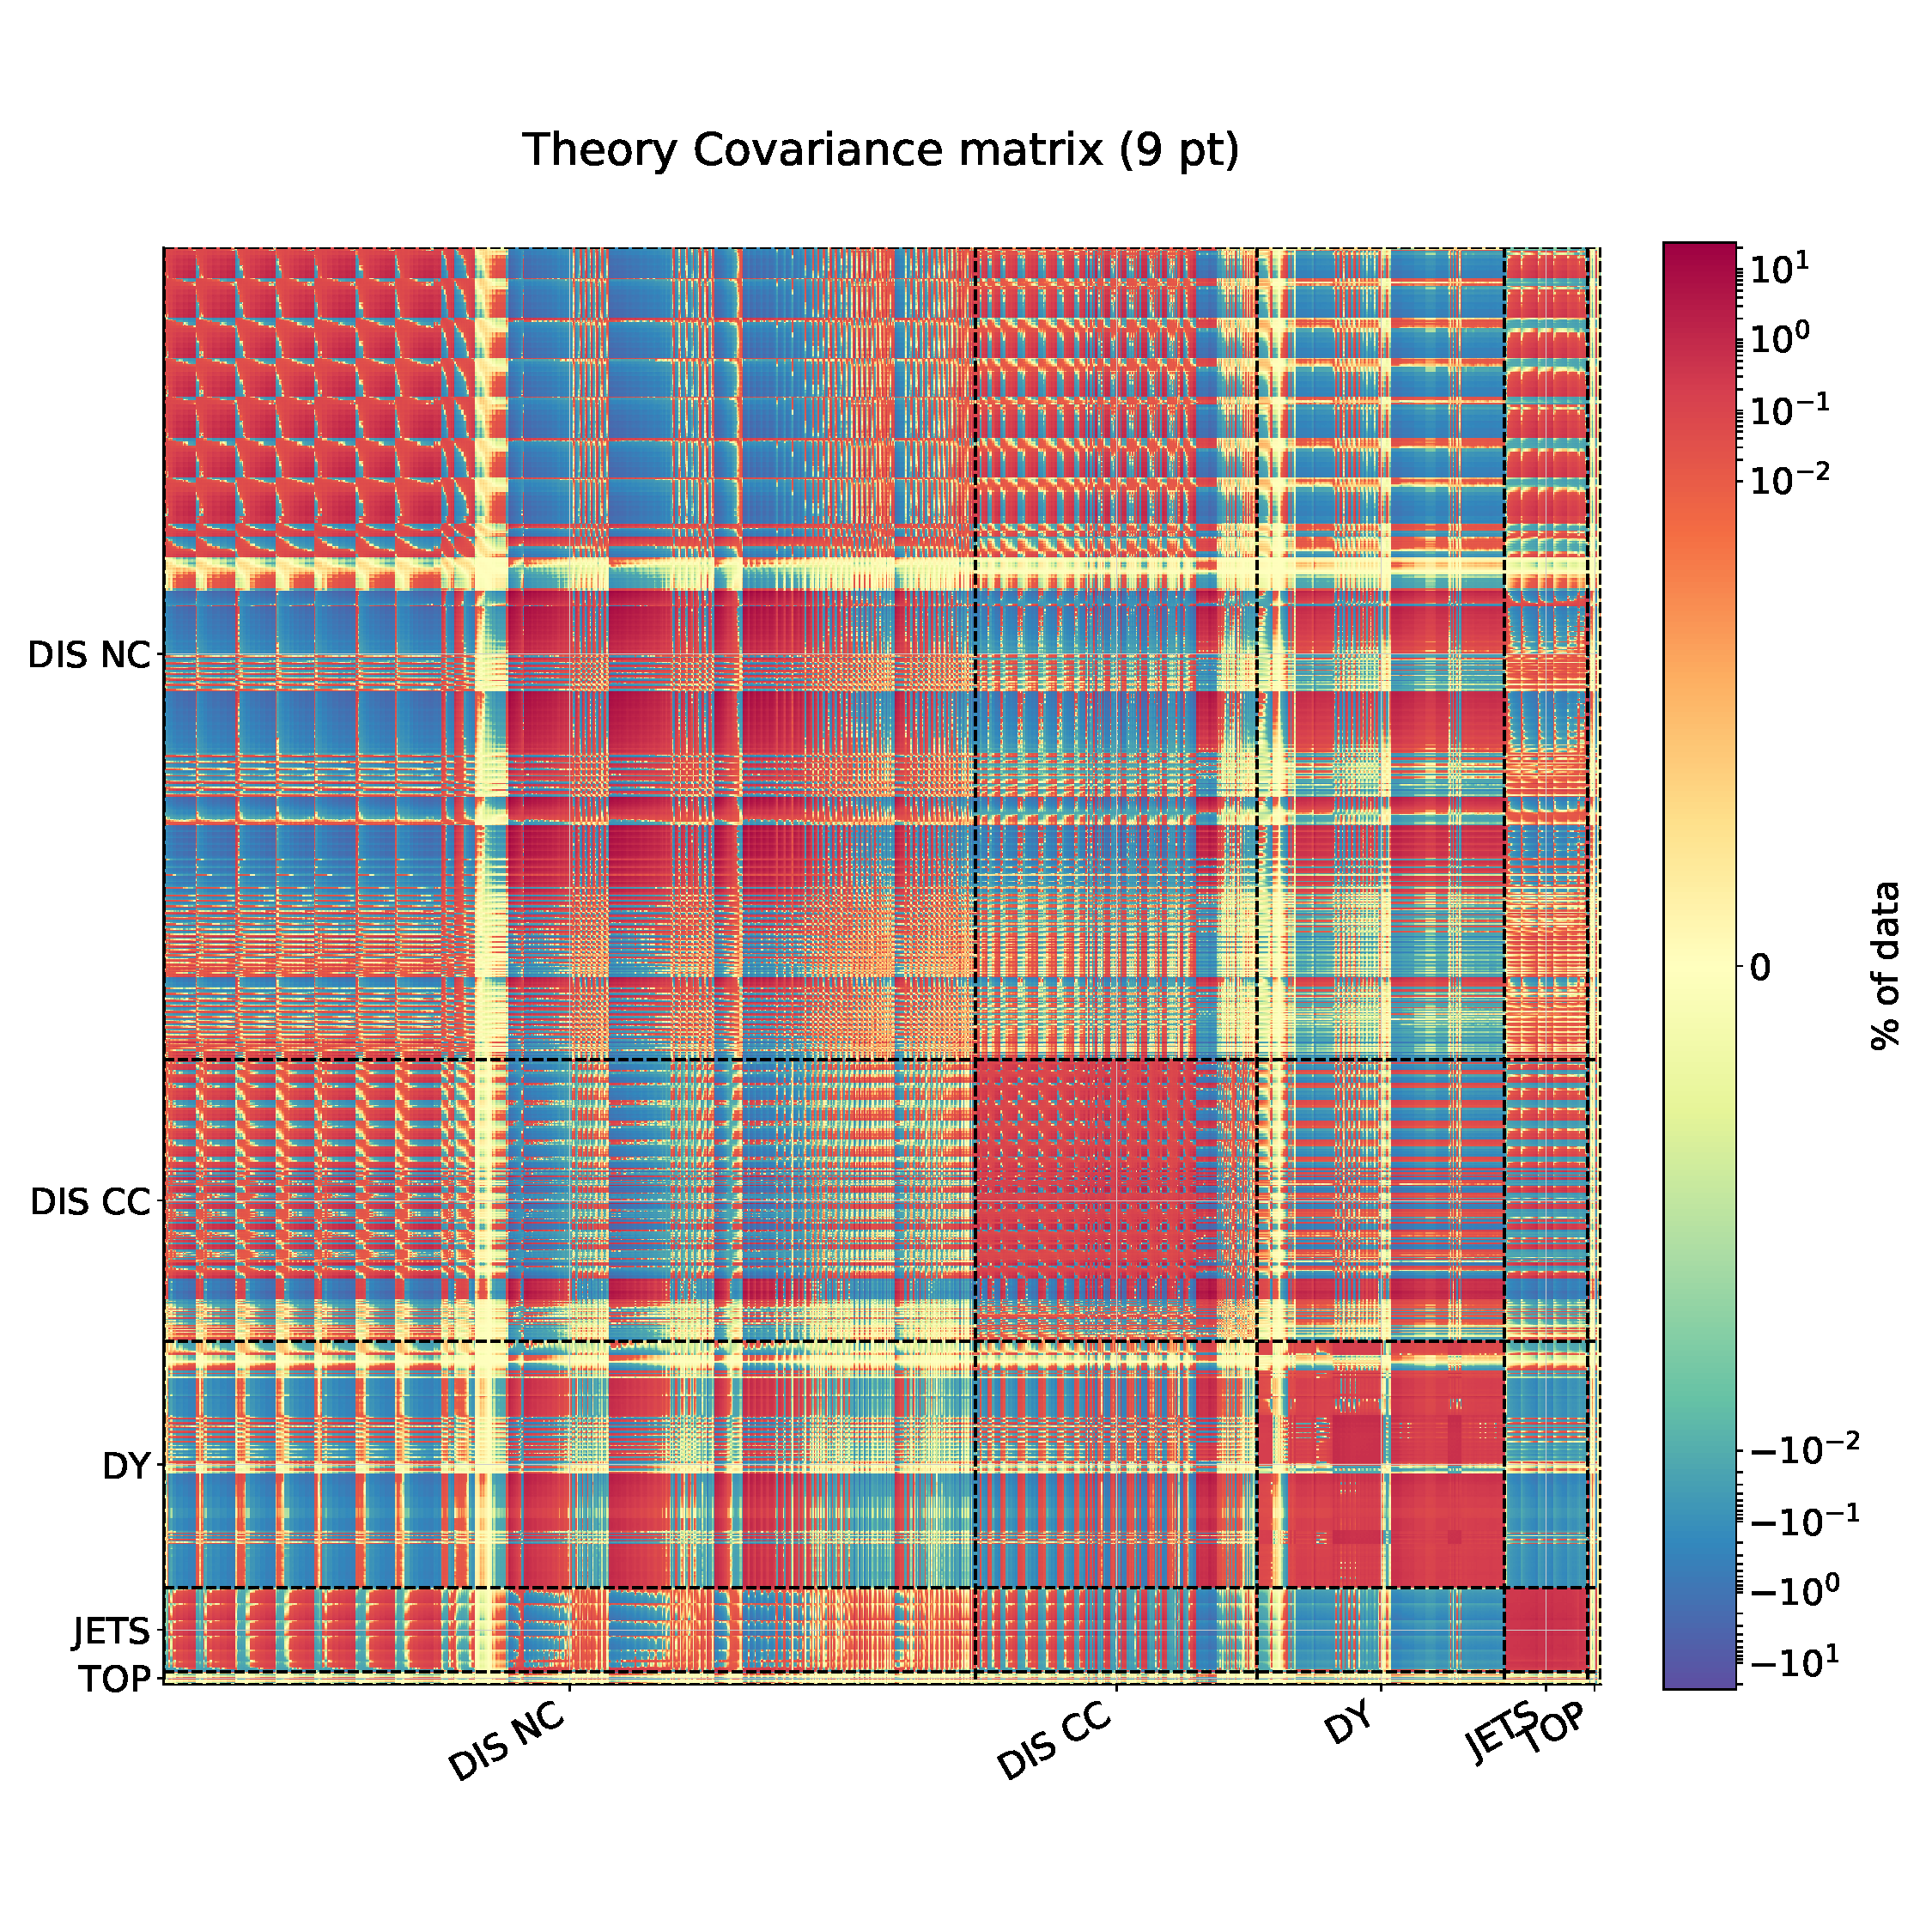
\includegraphics[width=0.49\linewidth]{mhous/plots/th_covmat_9pt.pdf}
    \caption{\label{fig:covmats}\small Comparison of the  experimental $C_{ij}$ (left)
      and the 9-point theoretical  $S_{ij}$  
      (right) covariance matrices.
      %
      Entries are displayed as a percentage of the experimental value.
      }
  \end{center}
\end{figure}
%%%%%%%%%%%%%%%%%%%%%%%%%%%%%%%%%%%%%%%%%%%%%%%%%%%%%%%%%%%%%%%%%%%%%%
We can also explore the structure of correlations between data points by viewing the covariance matrices as a whole. 

In Fig.~\ref{fig:covmats} we show $C$ alongside $S$ (9-point) as a $\%$ of experimental data value. It is immediately obvious that $S$ contains a much richer and more vibrant structure than $C$; experimental correlations only exist within experiments as the experiments are isolated from one another. However, predictions for these experiments originate from a common theoretical framework, and therefore theory uncertainties can exist between any two data points, regardless of experimental origin. In particular, data points within the same process are assigned a common renormalisation scale, inducing correlations between them. Furthermore, all points are predicted using the same PDFs and, in the 9-point prescription, share a common factorisation scale. This introduces entries in $S$ outwith individual processes. Along the block diagonal we note that correlations within an individual experiment are broadly positive, due to these points sharing a close kinematic region. In other regions we see a mixture of positive and negative correlations, for example HERA is generally positively correlated with DY but negatively correlated with fixed target DIS. 
%%%%%%%%%%%%%%%%%%%%%%%%%%%%%%%%%%%%%%%%%%%%%%%%%%%%%%%%%%%%%%%%%%%%%
\begin{figure}[H]
  \begin{center}
    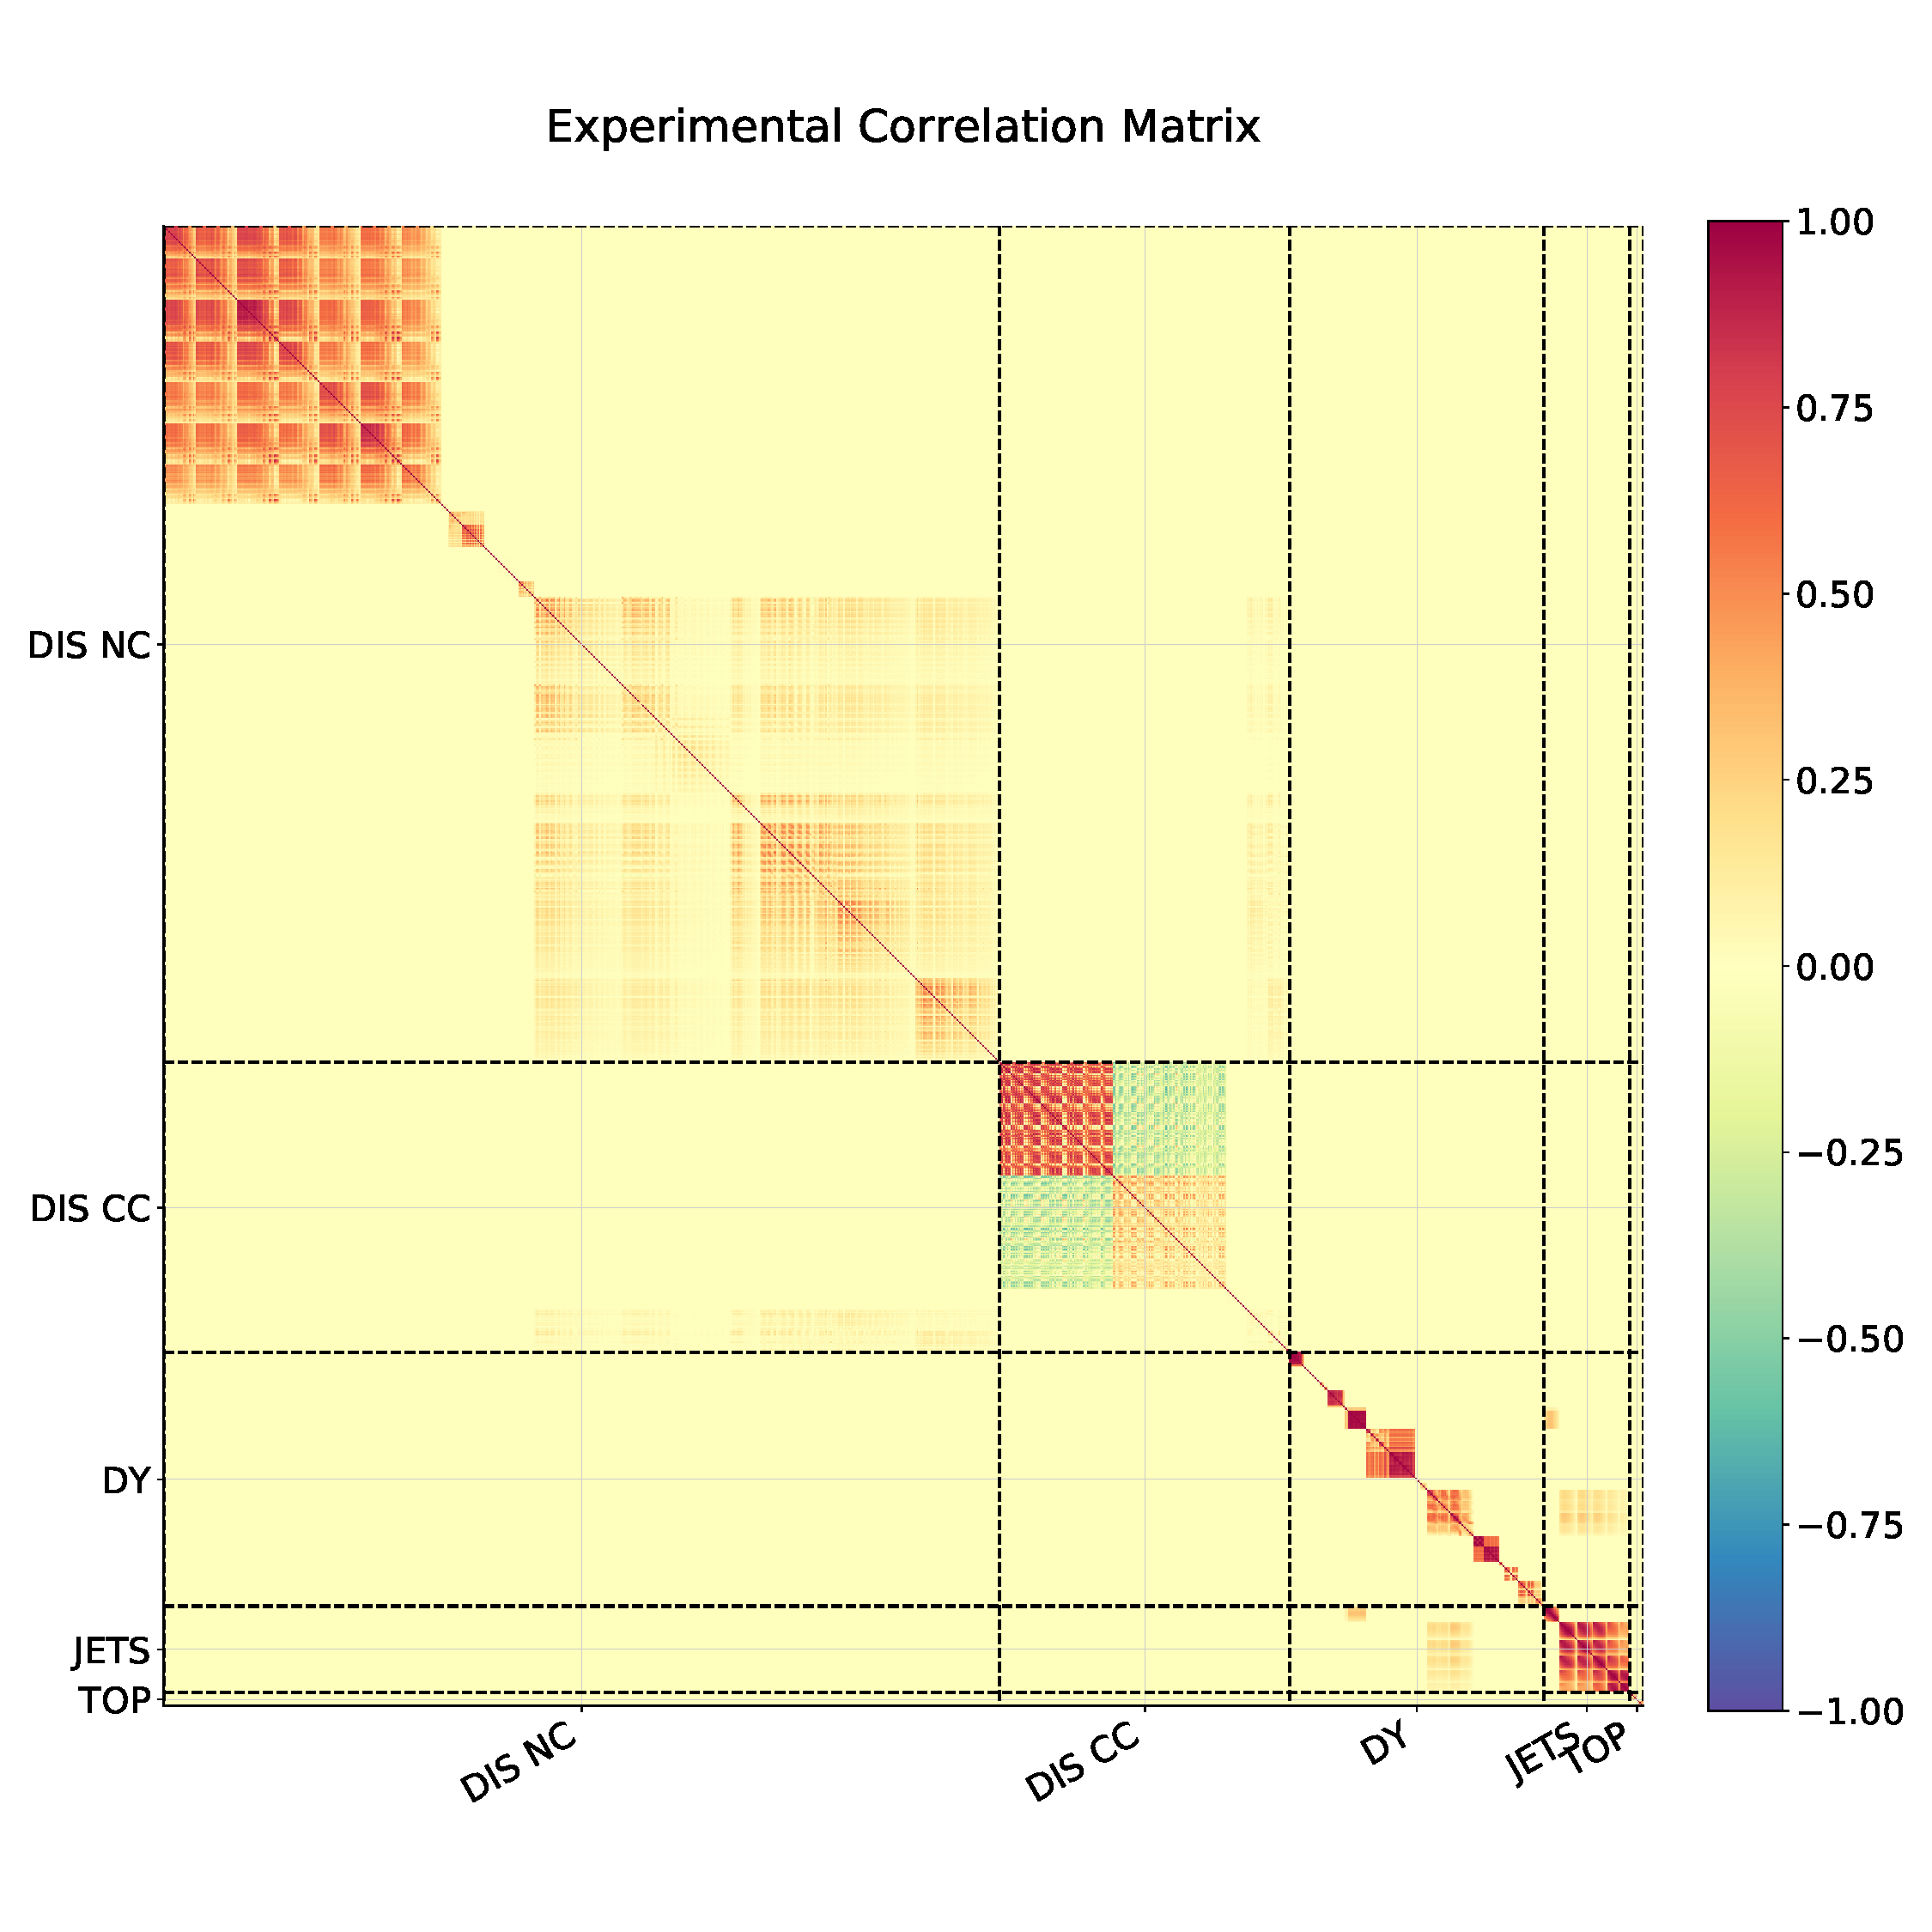
\includegraphics[width=0.49\linewidth]{mhous/plots/exp_corrmat.pdf}
    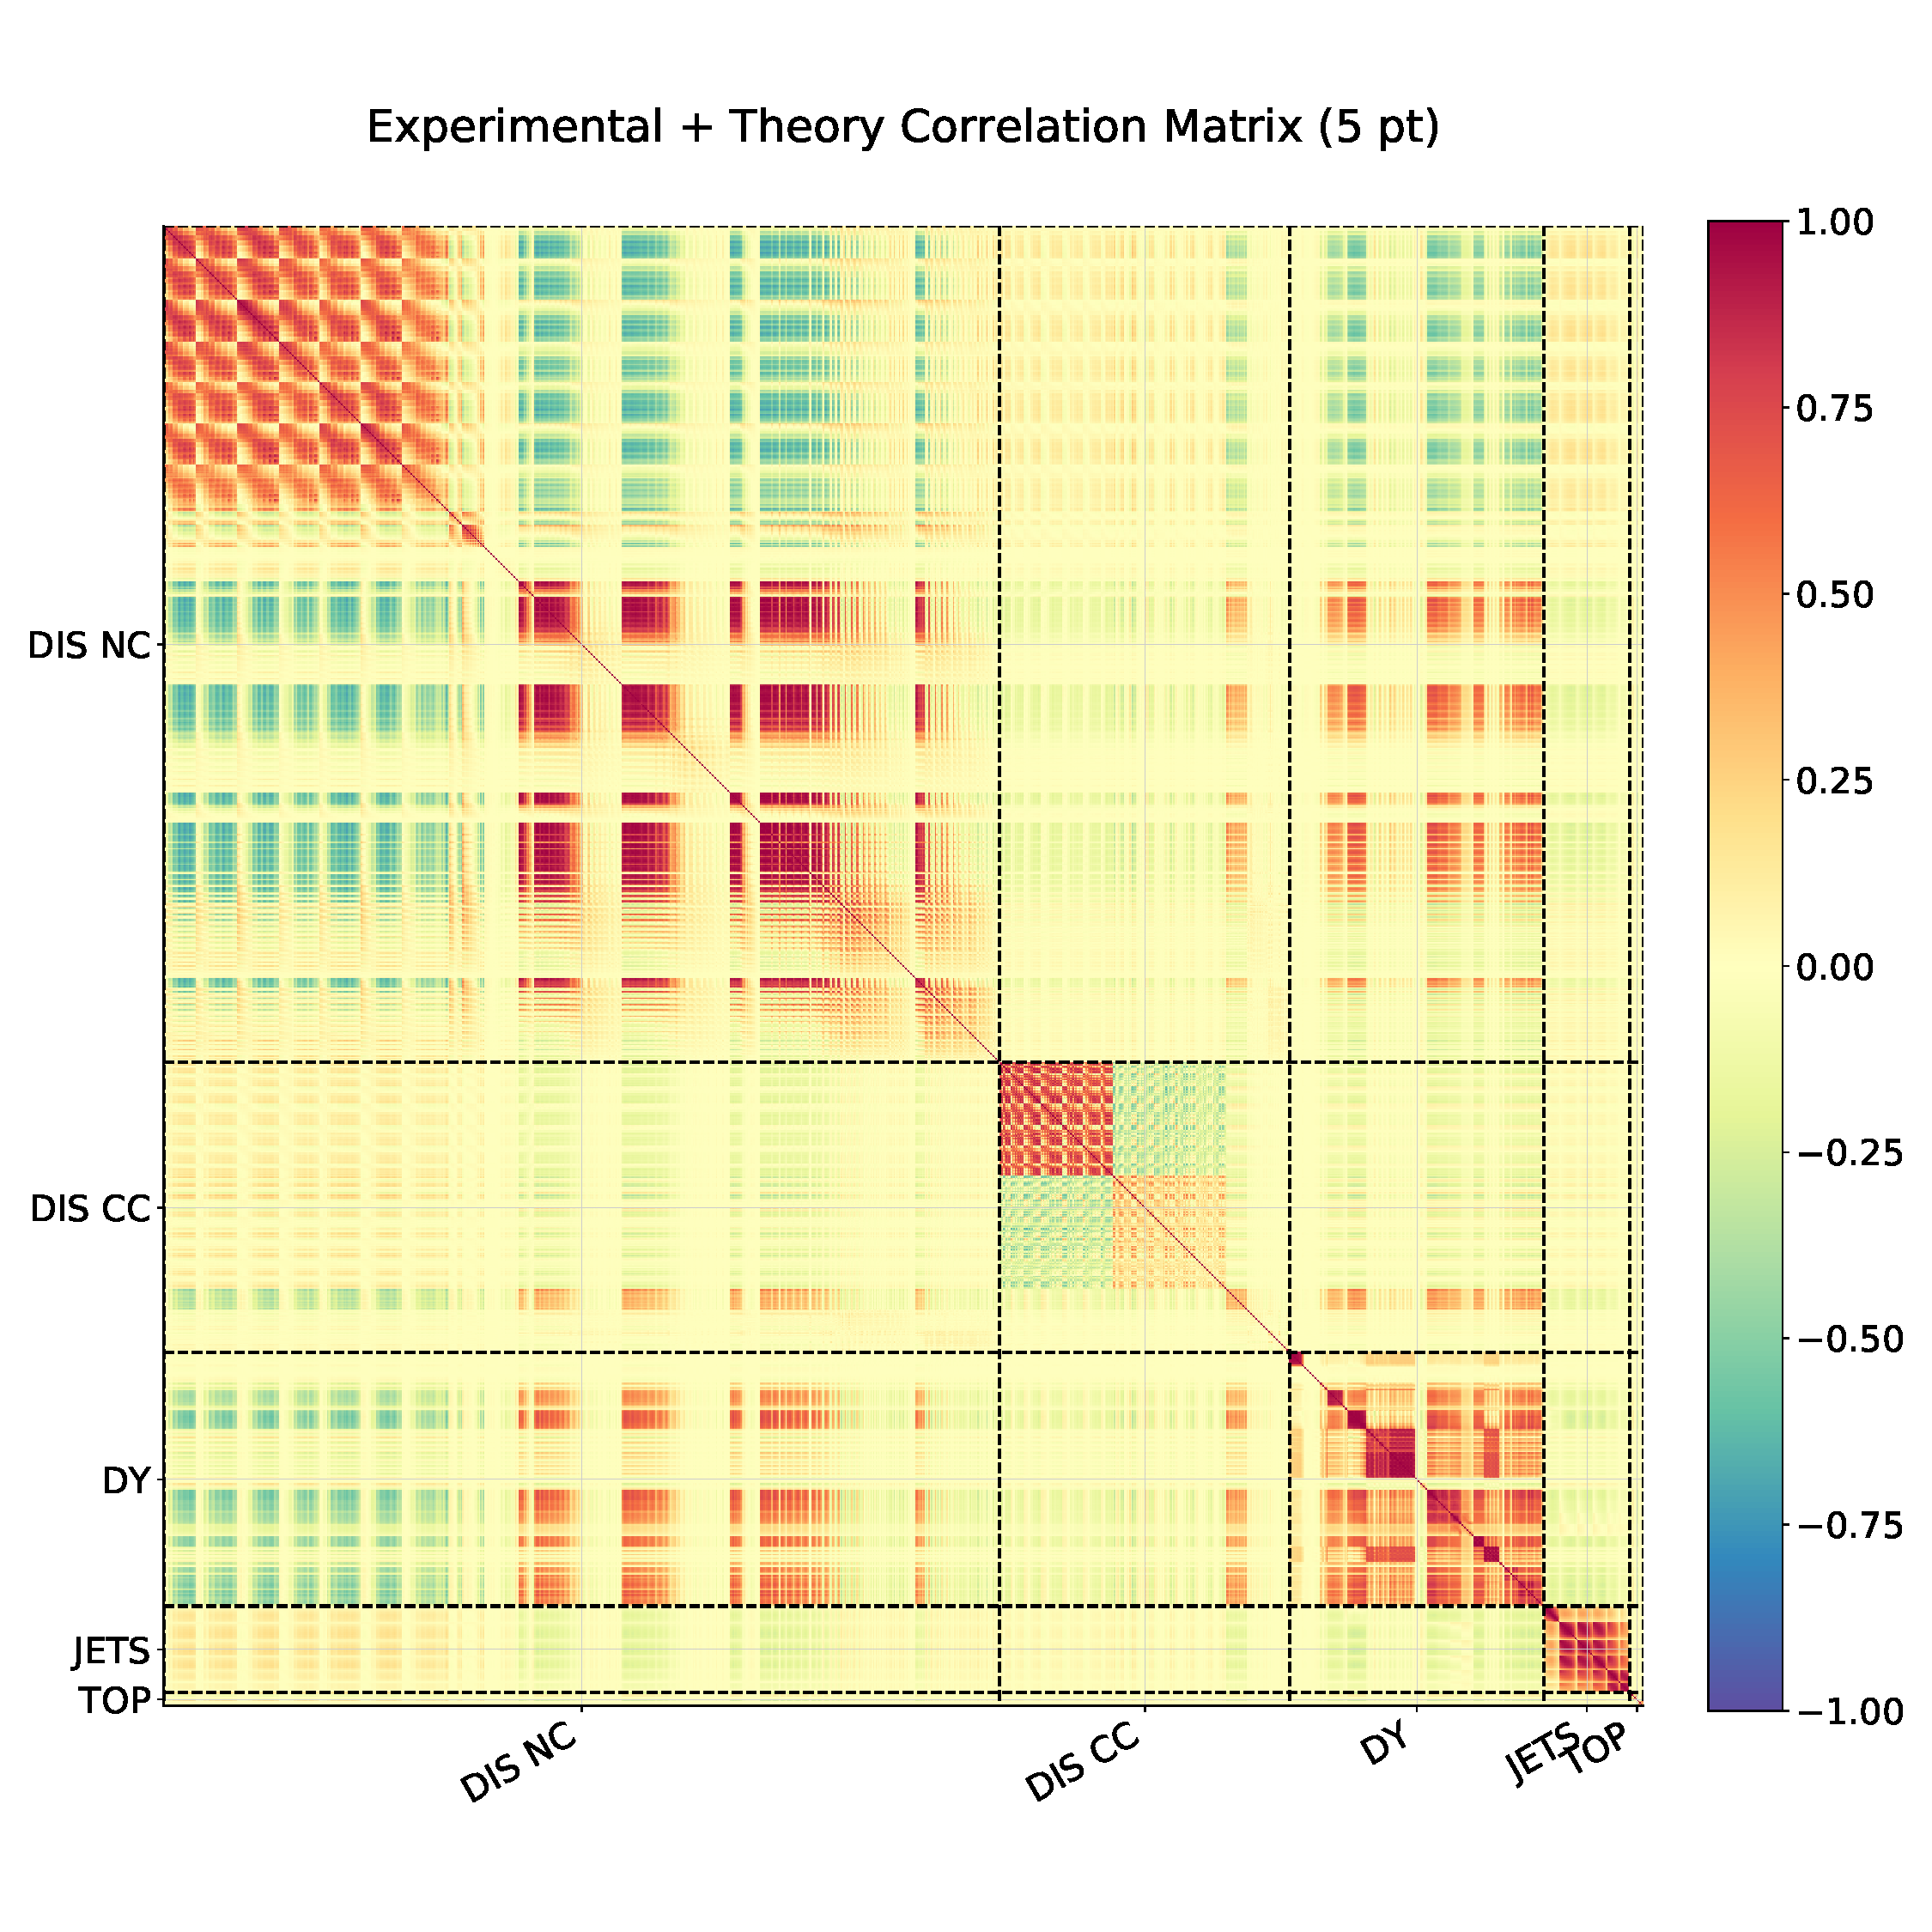
\includegraphics[width=0.49\linewidth]{mhous/plots/expth_corrmat_5pt.pdf}
\vskip-0.5cm
    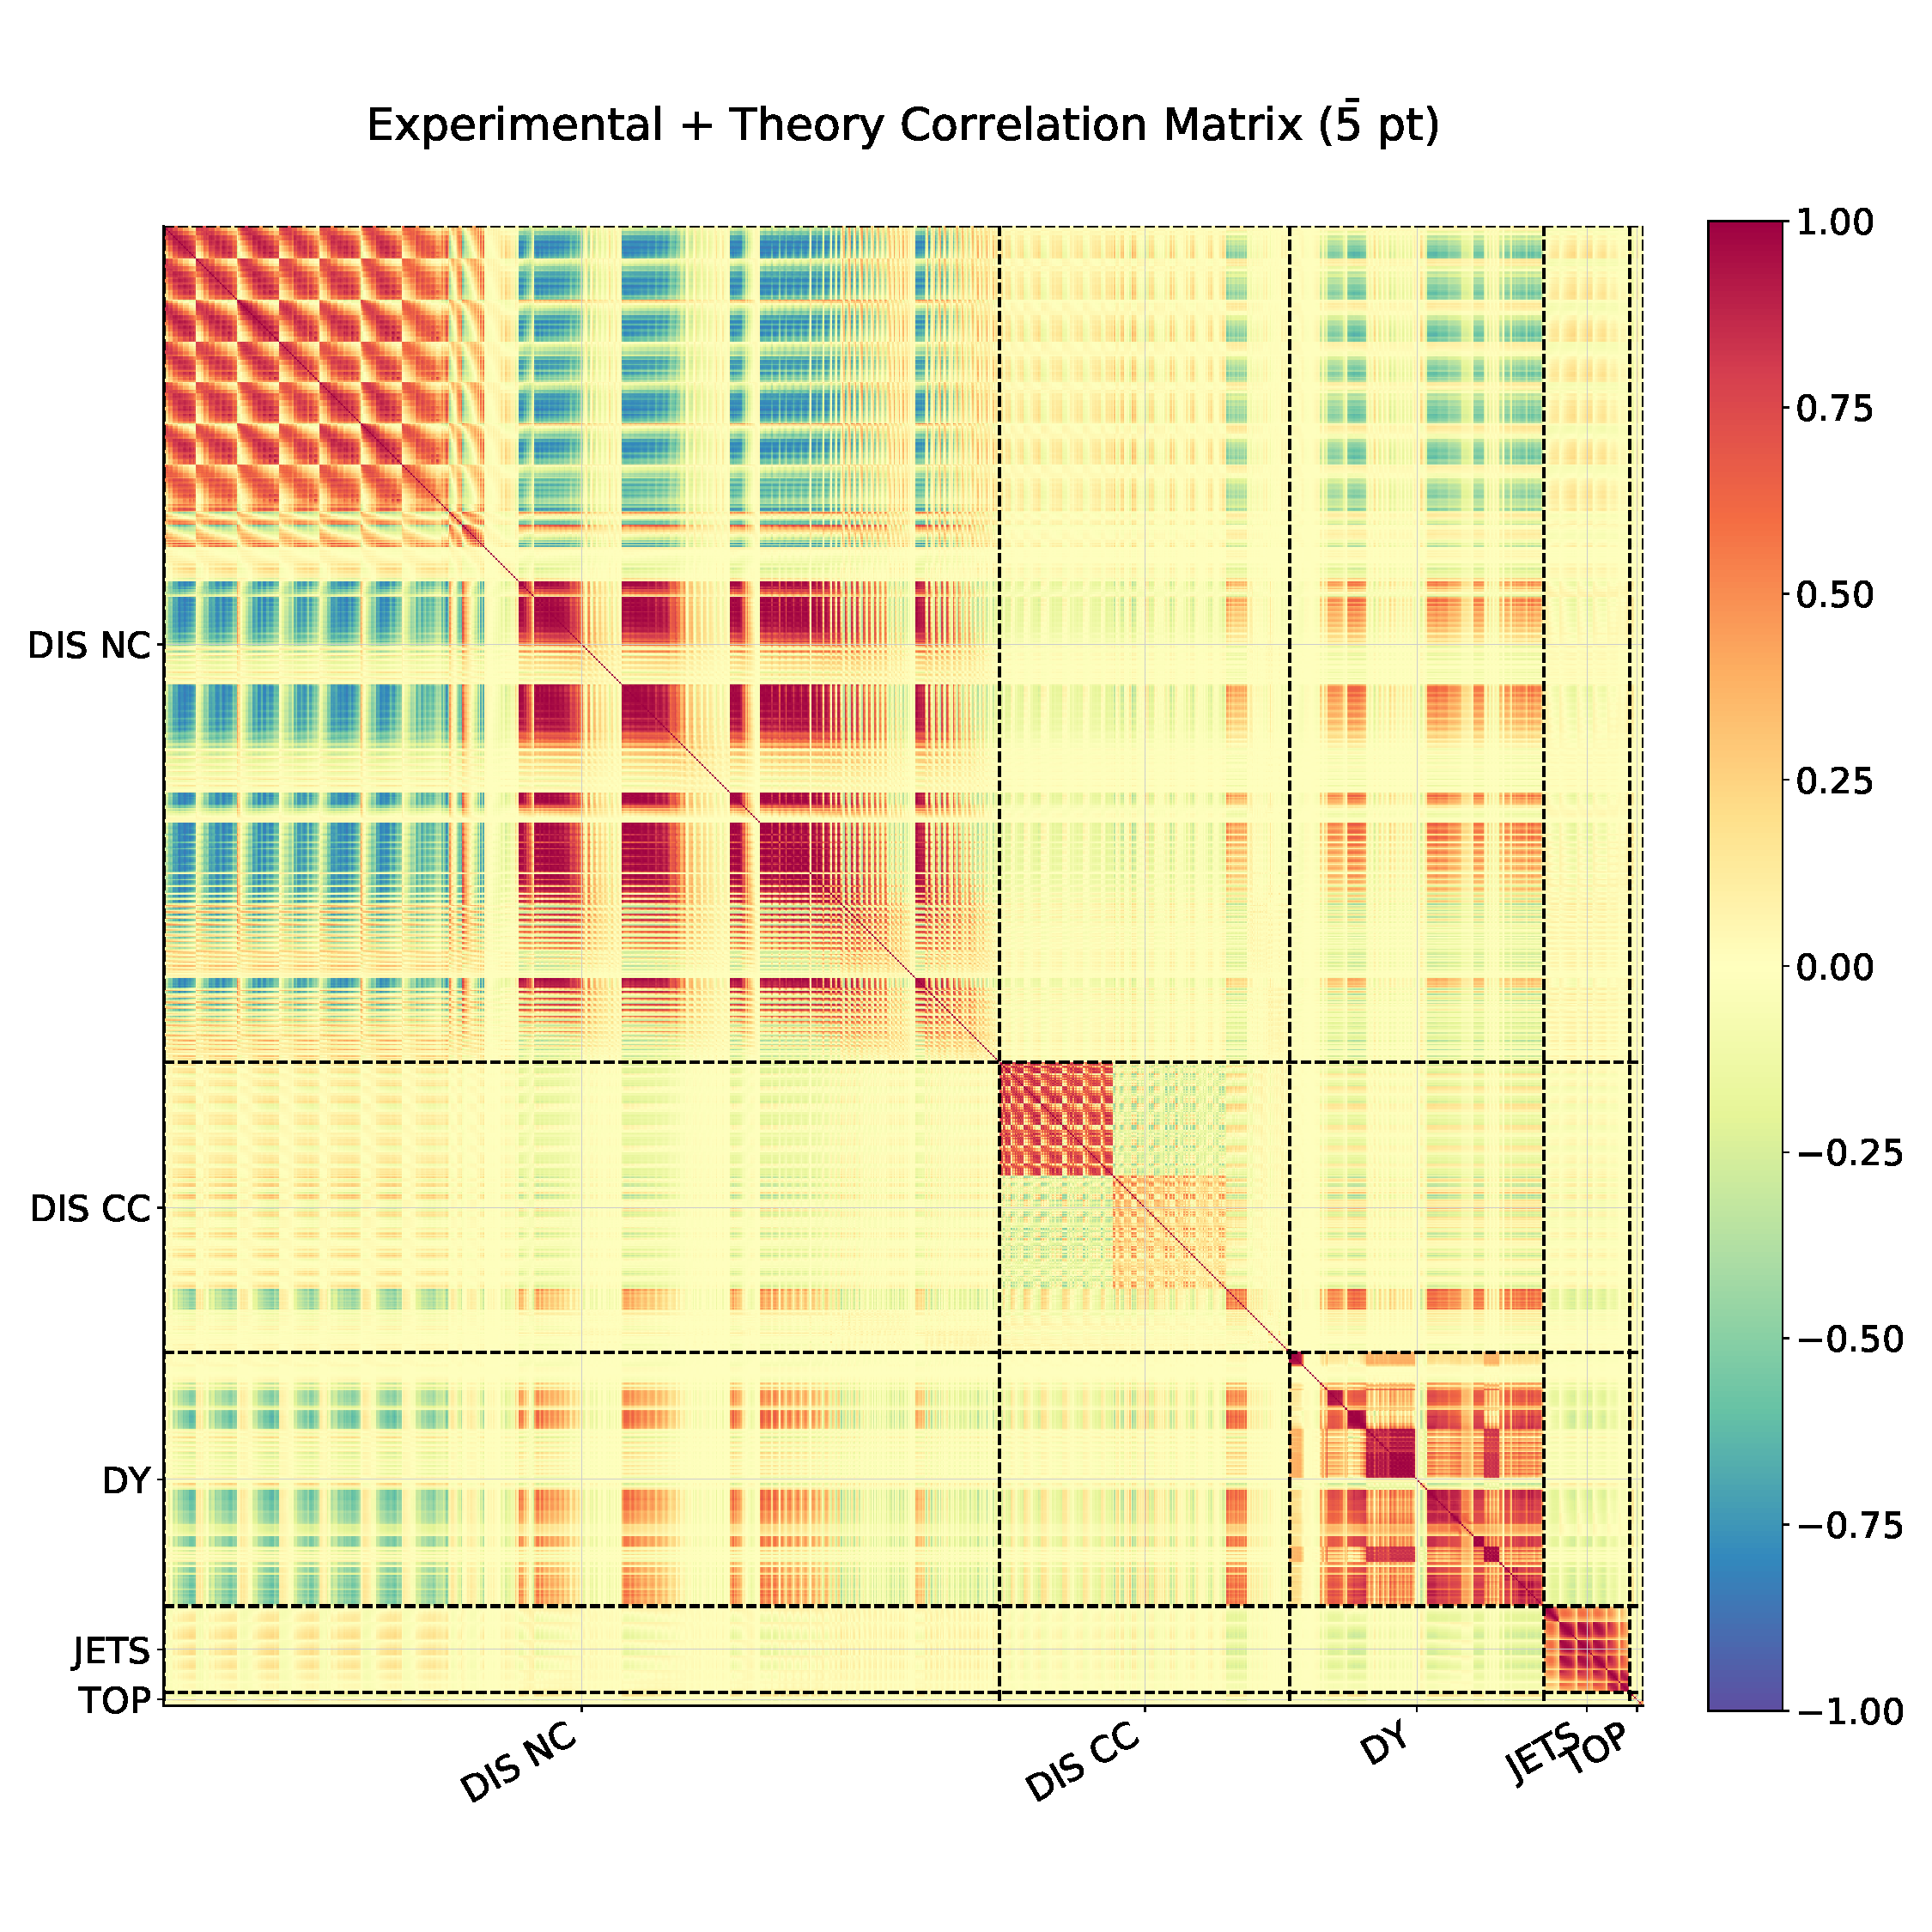
\includegraphics[width=0.49\linewidth]{mhous/plots/expth_corrmat_5barpt.pdf}
    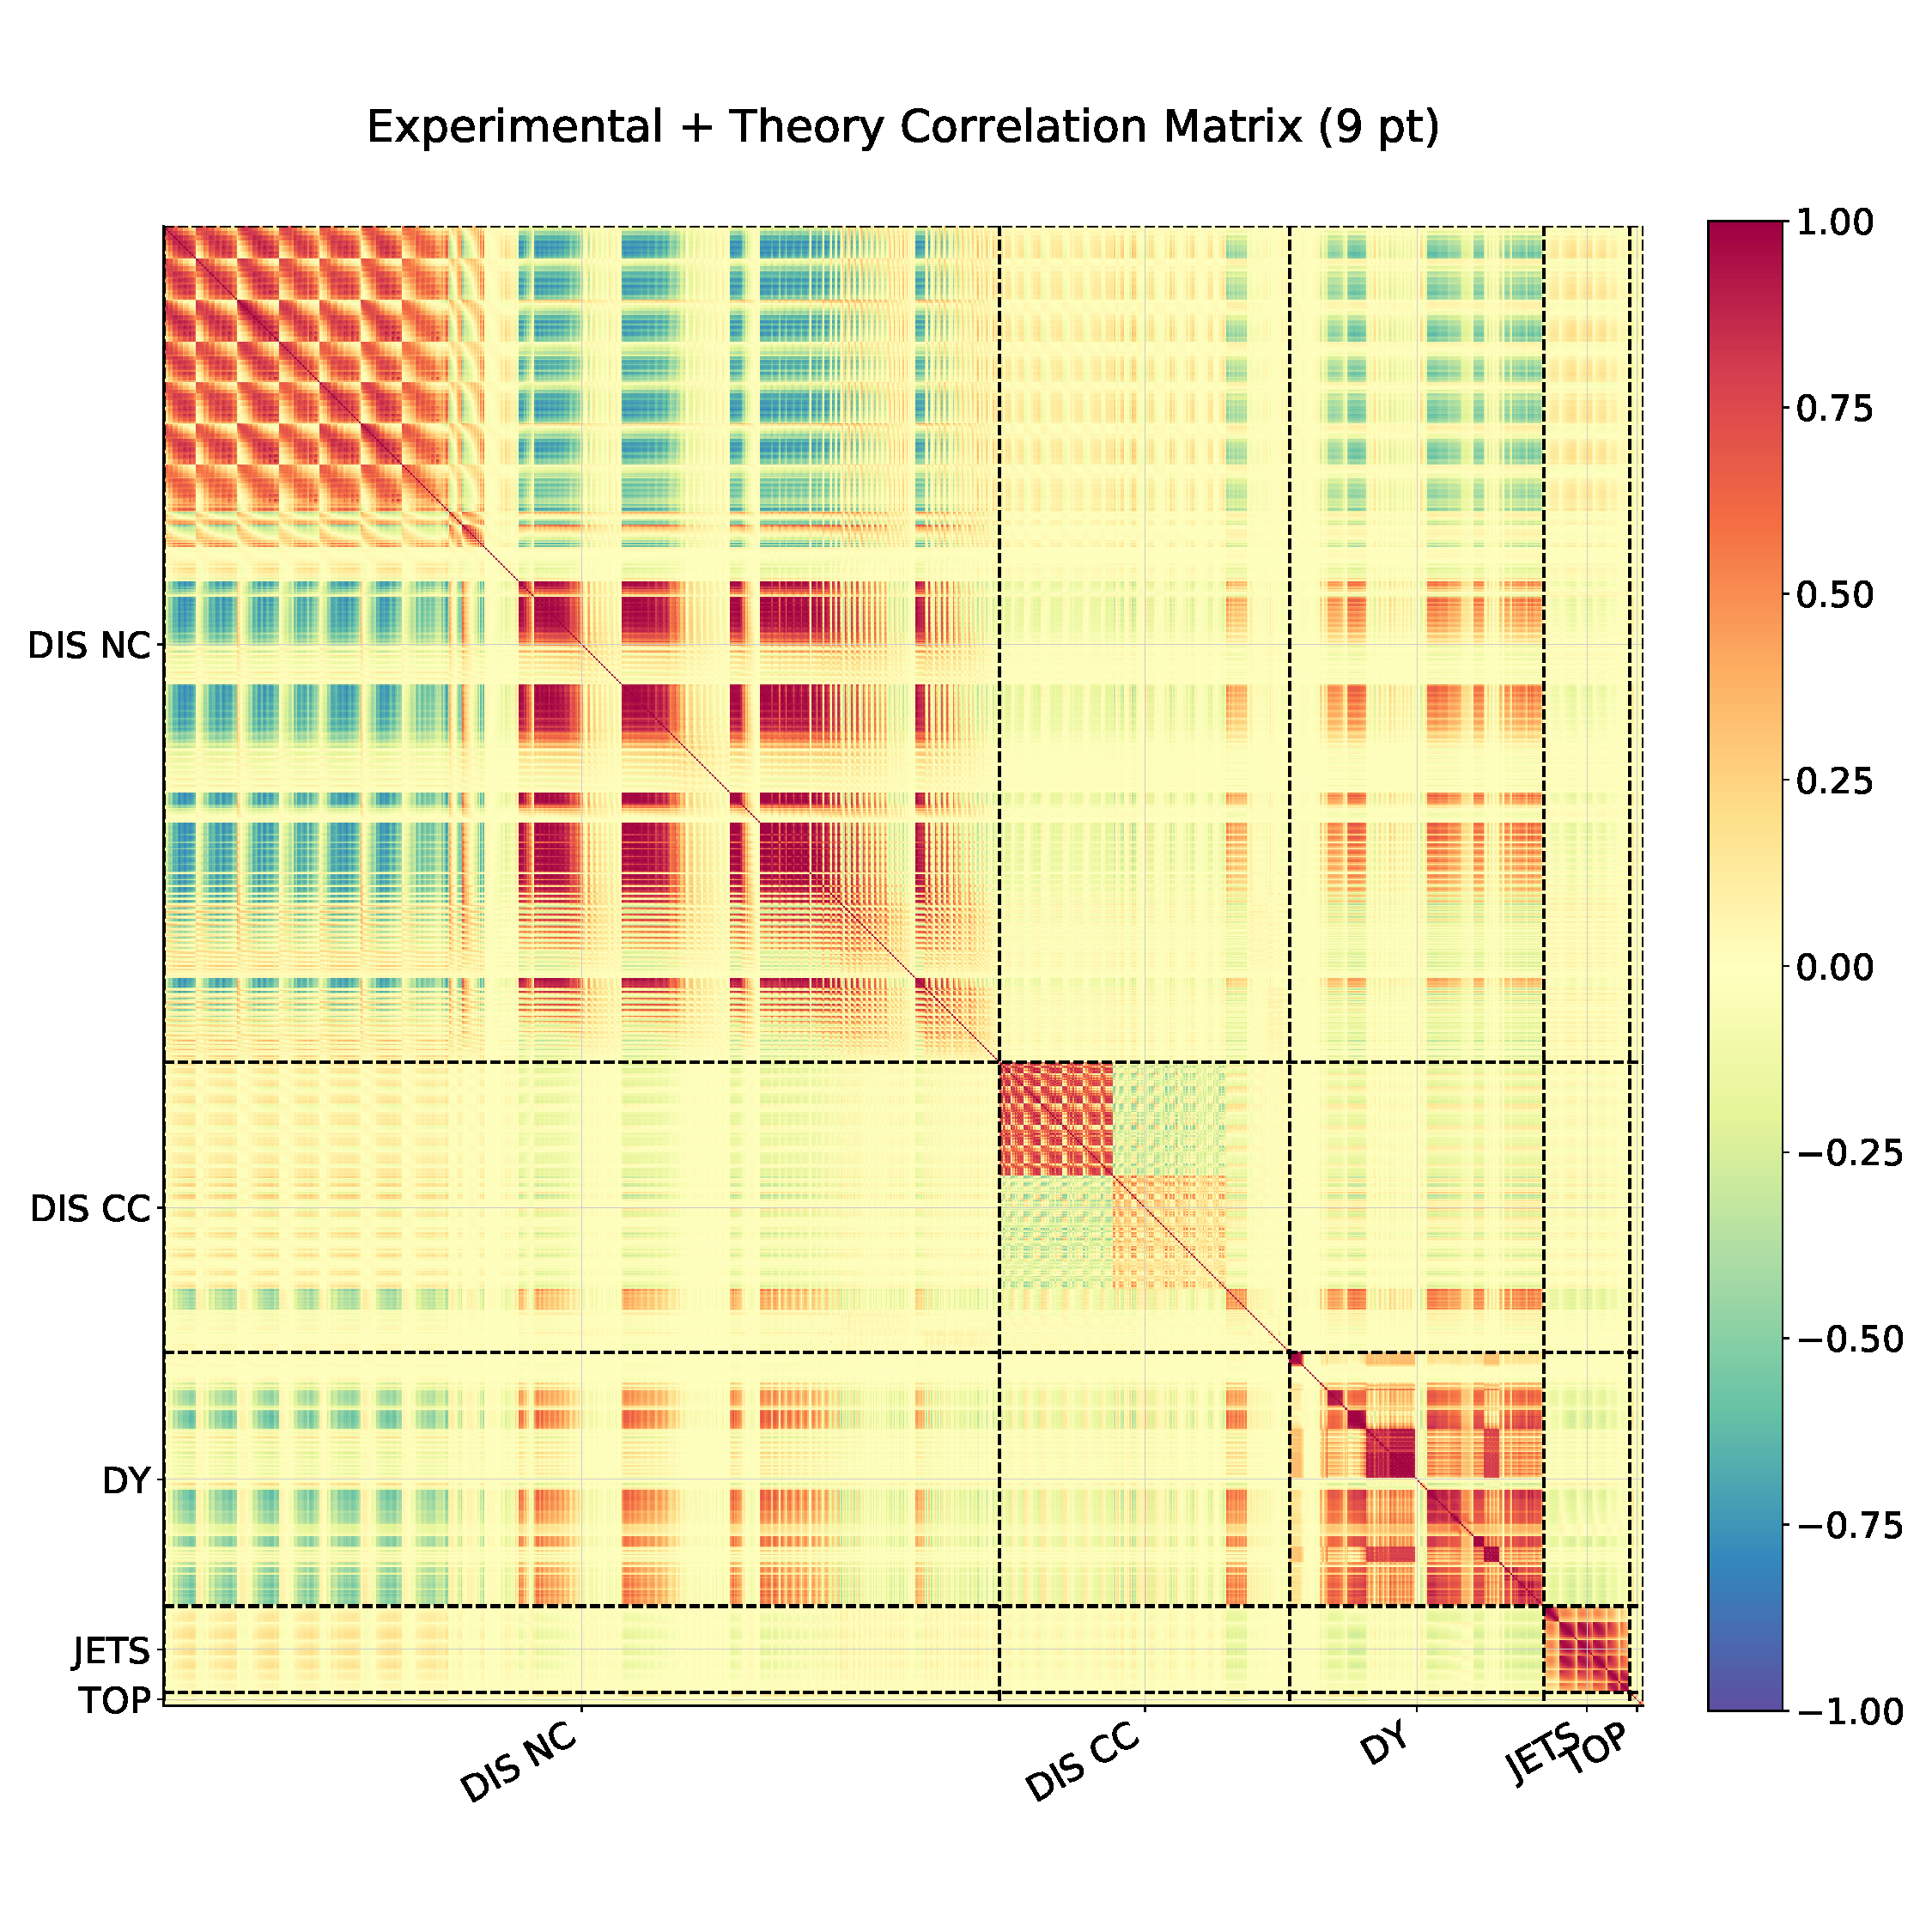
\includegraphics[width=0.49\linewidth]{mhous/plots/expth_corrmat_9pt.pdf}
\vskip-0.5cm
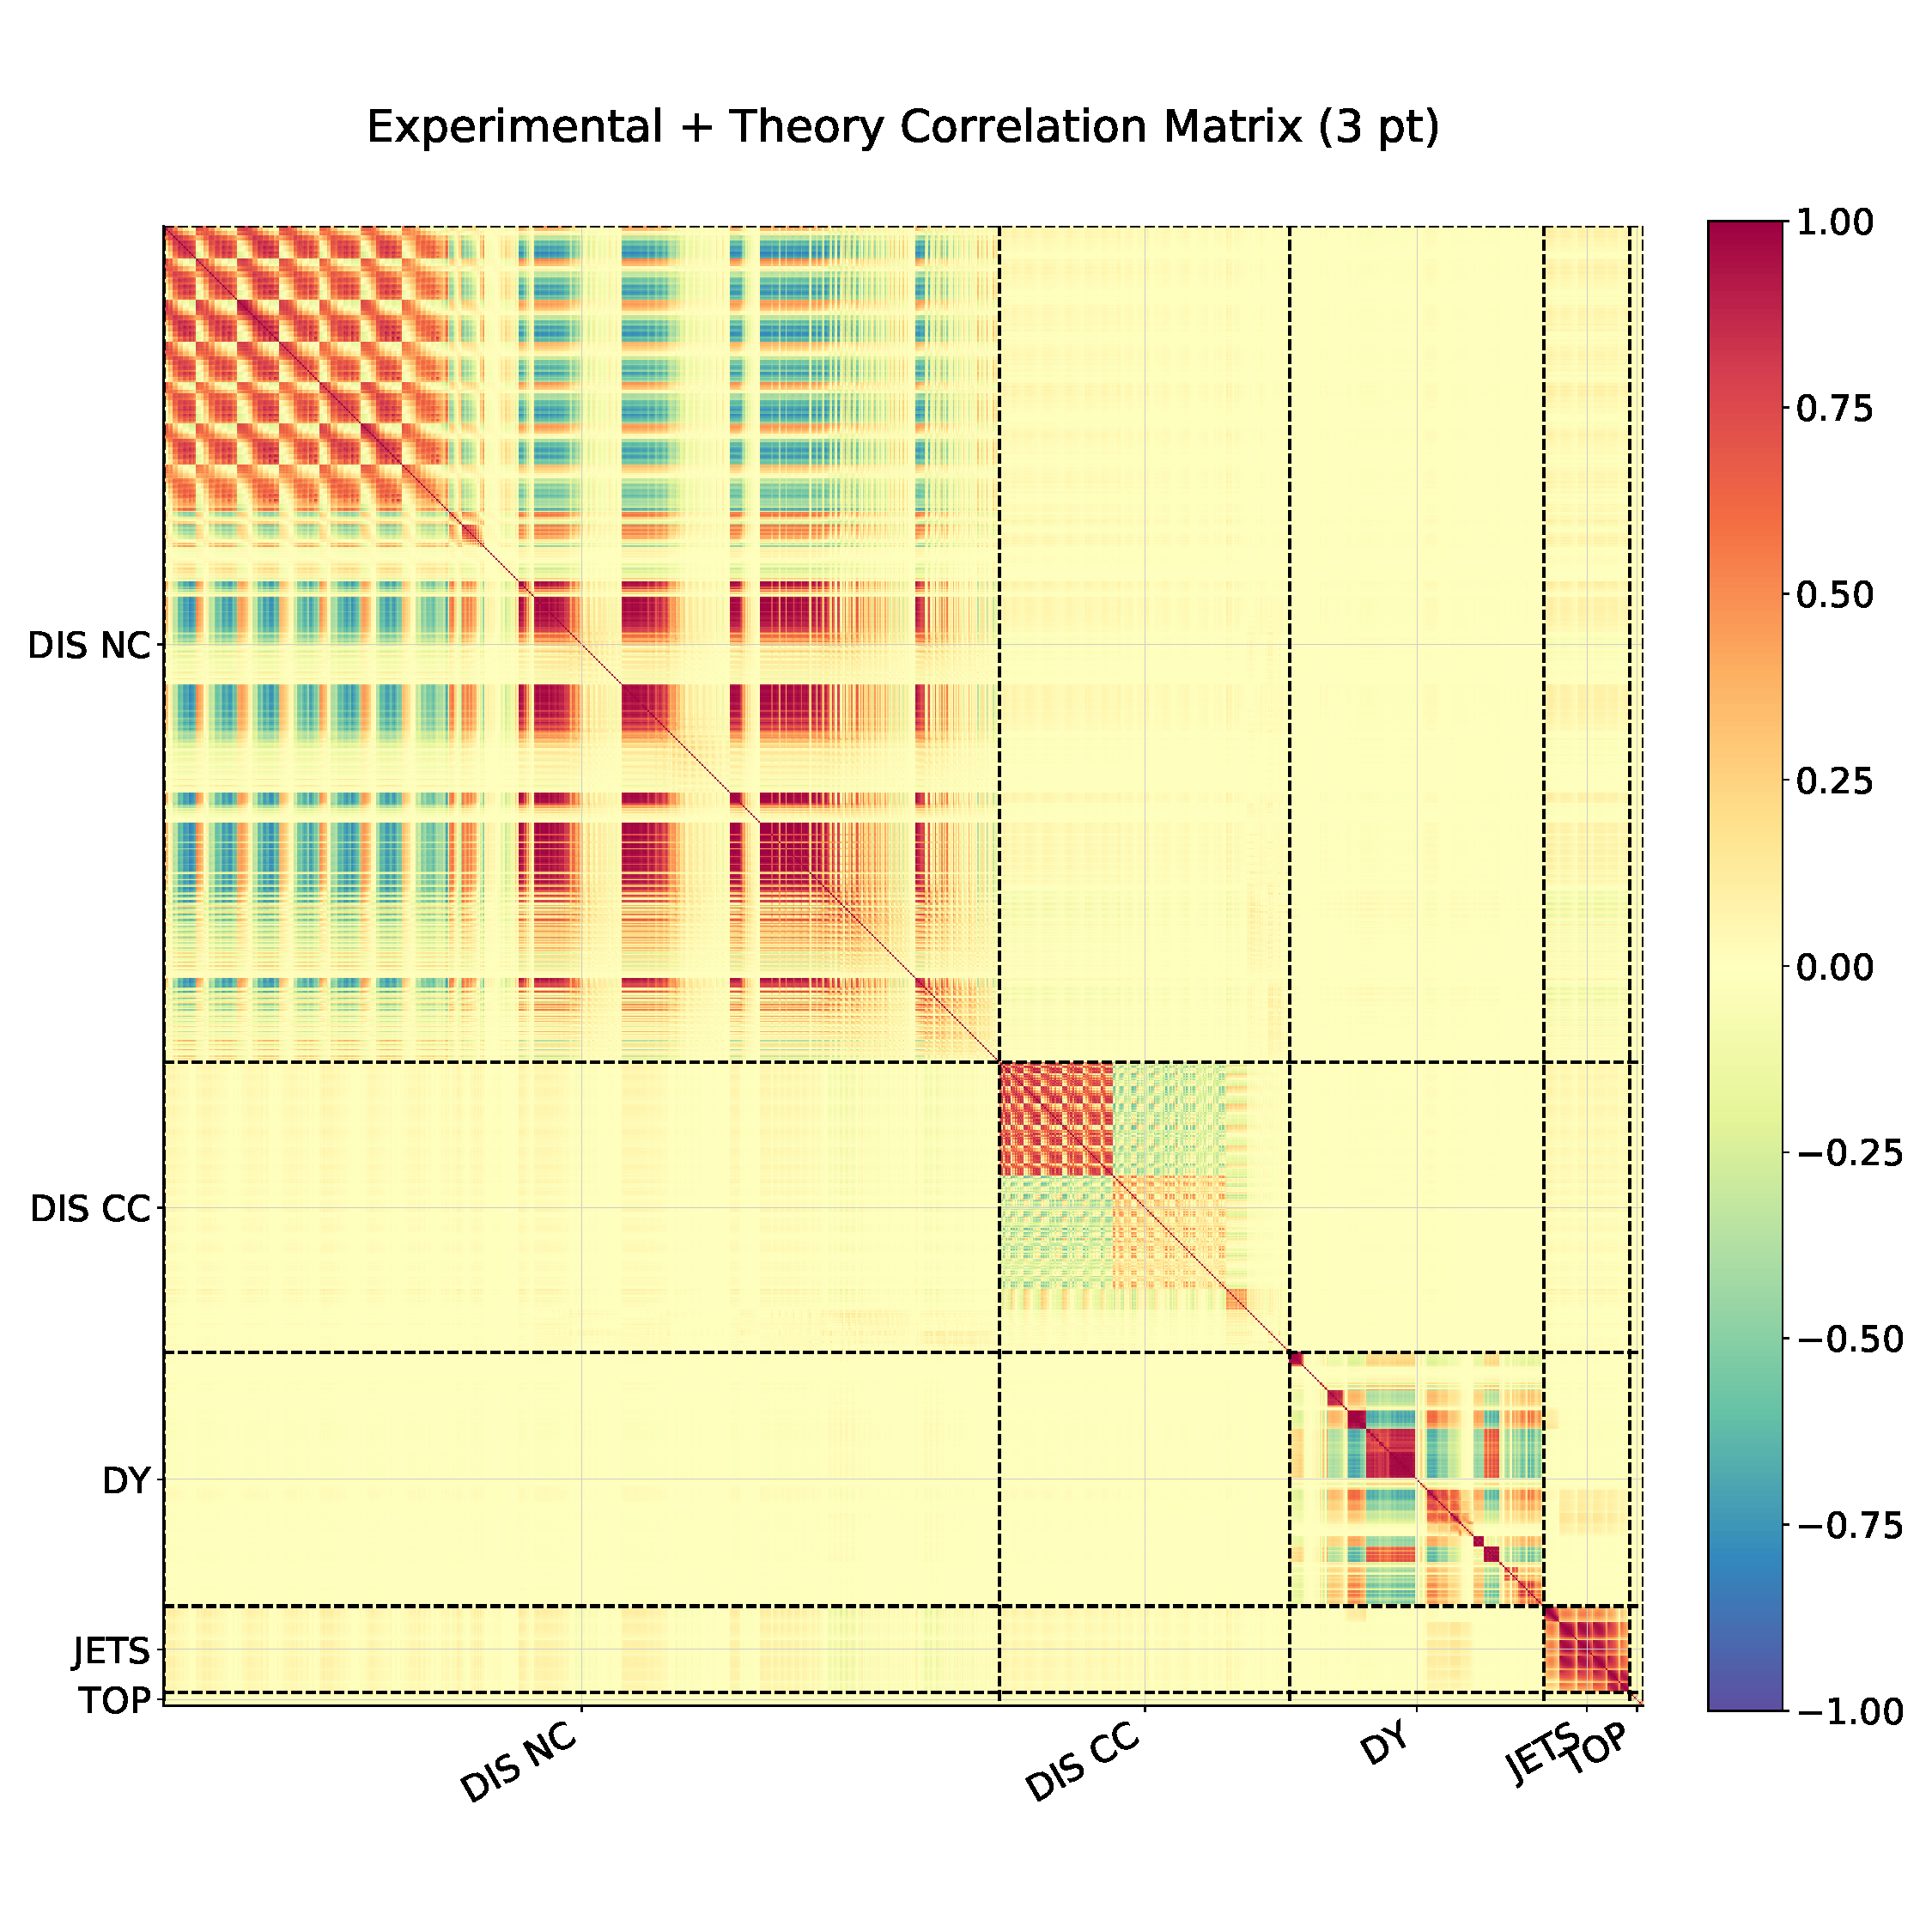
\includegraphics[width=0.49\linewidth]{mhous/plots/expth_corrmat_3pt.pdf}
    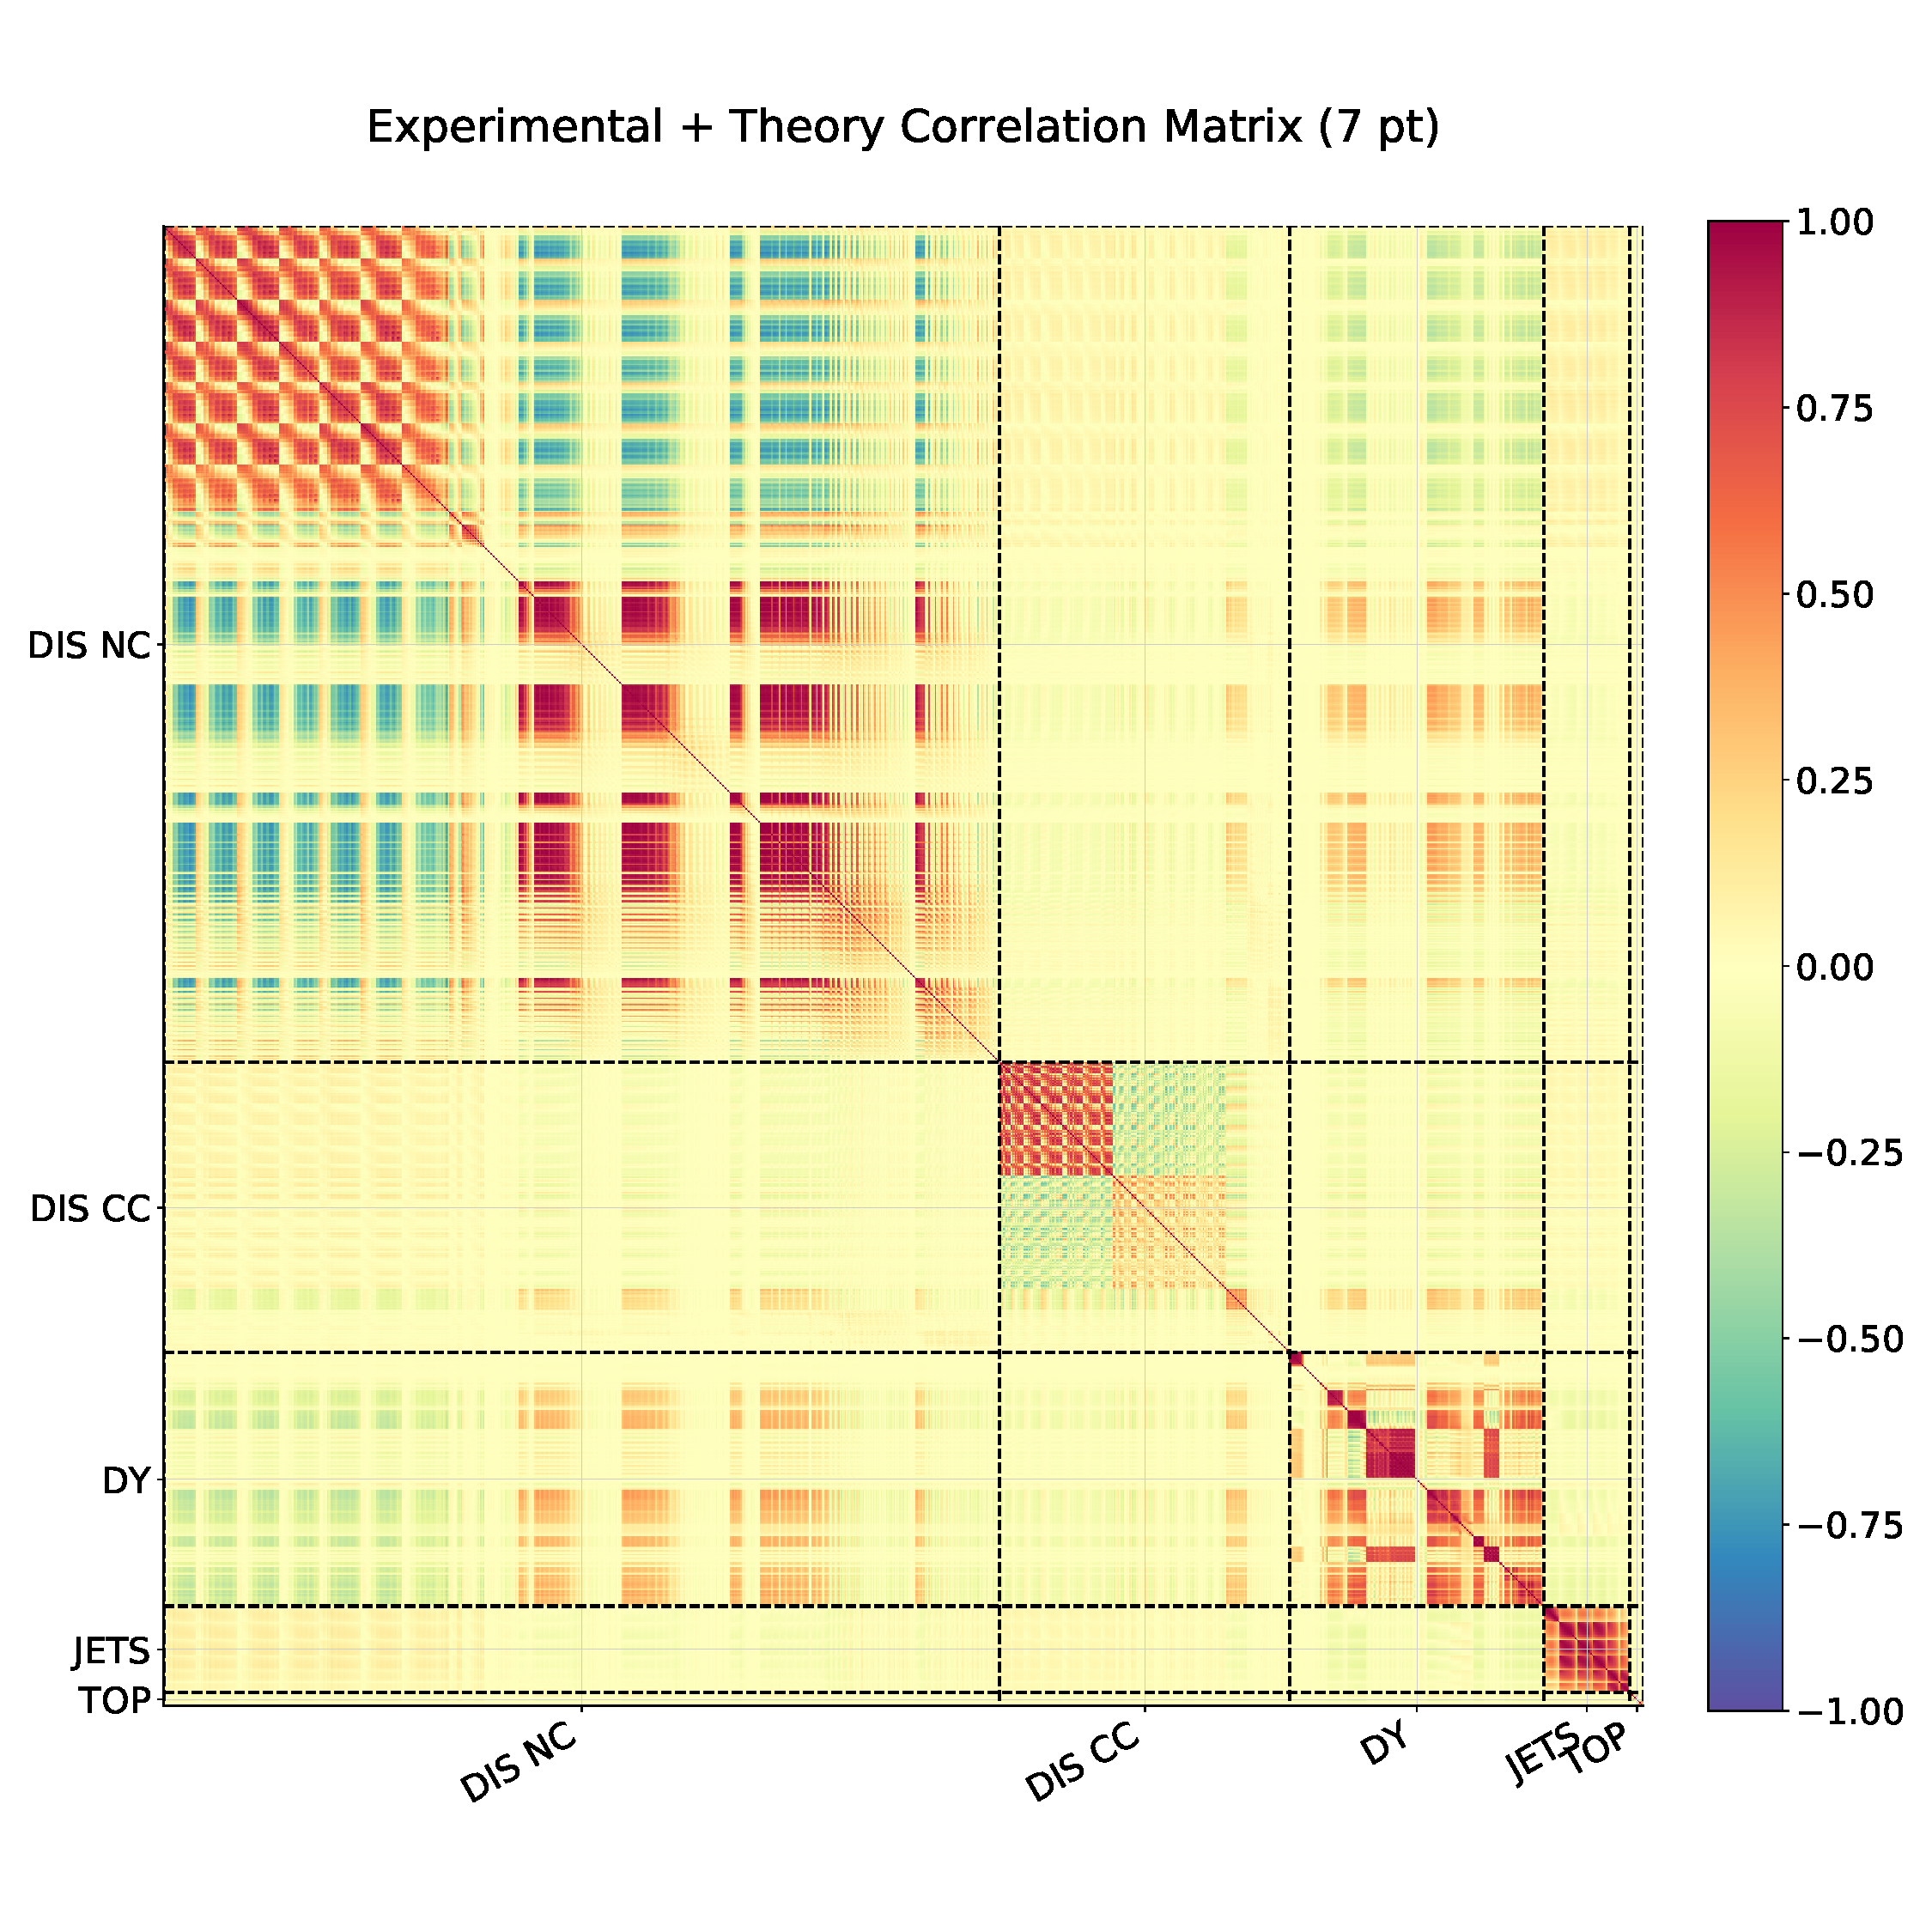
\includegraphics[width=0.49\linewidth]{mhous/plots/expth_corrmat_7pt.pdf}
    \caption{\small Comparison of the experimental correlation matrix (top left) and the
      the combined experimental and theoretical correlation matrices computed using the prescriptions described in Sec.~\ref{sec:prescrip}: the symmetric prescriptions (5-pt top right, $\overline{5}$-pt centre left, 9-pt centre right); and asymmetric prescriptions (3-pt bottom left, 7-pt bottom right).
  \label{fig:corrmats} }
  \end{center}
\end{figure}
%%%%%%%%%%%%%%%%%%%%%%%%%%%%%%%%%%%%%%%%%%%%%%%%%%%%%%%%%%%%%%%%%%%%%%
The exact structure of $S$ is dependent on the chosen prescription in Sec.~\ref{sec:prescrip}. In Fig.~\ref{fig:corrmats} we delve into these differences by comparing correlation matrices for each prescription, defined
\be
\text{corr}^A_{ij} \equiv \frac{A_{ij}}{\sqrt{A_{ii}}\sqrt{A_{jj}}}.
\ee
This removes the effect of the differing magnitude of entries, laying bare the underlying structure; a value of 1 corresponds to full correlation between two points, a value of 0 corresponds to no correlation and a value of -1 corresponds to full anticorrelation. This time we look at the impact of adding the theory covariance matrix to the experiement covariance matrix. In all cases a richer structure emerges, however we note that:
\begin{itemize}
\item For 3-point the correlations between processes are a lot weaker, and this is because both factorisation and renormalisation scale are uncorrelated between processes;
\item For 7-point (the other asymmetric prescription), the correlations are weaker than in 5-point despite the fact that 7-point uses the same scale variation points as 5-point plus two additional ones. This is because the $\mu_F$ variation is combined with the uncorrelated ``scale of process" variation;
\item All three symmetric prescriptions show similar patterns of correlation.
\end{itemize}
From this, it seems that any of the symmetric prescriptions might be a suitable choice. However, in the next section we outline more quantitative tests to validate whether or not each prescription provides a reasonable estimate of MHOUs, and hence determine the best prescription. 

\section{Validating the theory covariance matrix}
\label{sec:valid}
Whilst in general the structure of MHOs is unknown to us, due to the perturbative nature of calculations we do know that the MHOU is dominated by the next MHO; so at NLO we expect the MHOU to be dominated by the NNLO terms. A good test of the NLO theory covariance matrix, therefore, is that it reliably encapsulates the known NNLO predictions. In this section we describe a method of validation based on this observation.We summarise the procedure here, before going into some considerable detail in Sec.~\ref{subsec:val_details}. 

We consider the space of experimental data, $D$, spanned by the vector of experimental data points, $D_i$, $i=1,\dots, N_{dat}$. The theory covmat, $S_{ij}$ acts as a linear operator on this space. We know that $S_{ij}$ is positive semi-definite and symmetric, and therefore has positive or zero eigenvalues only. As an uncertainty matrix, $S_{ij}$ defines ellipsoids, $E$, of given confidence level. These lie in the subspace $S \in D$, and are centred on the NLO prediction, $T_i^{NLO}$. A test of the efficacy of $S_{ij}$ is that the 1-$\sigma$ ellipse broadly encapsulates the known shift to the next higher order, $\delta_i \sim T_i^{NNLO} - T_i^{NLO}$. Note that here $T_i^{NNLO}$ must be evaluated using the same NLO PDF, to ensure that the shift is due only to perturbative differences and not to effects from refitting. This is a robust test, owing to the great difference between $\text{dim}\ D\ \sim 1000$ and $\text{dim}\ S\ \sim 10$; for a random matrix we would expect only 1\% of $\delta_i$ to lie in $S$. 

\subsection{Details of validation procedure}
\label{subsec:val_details}
Recall that the ellipse $E \in S \in D$, where $\text{dim}\ D\ = N_{dat}$ and $\text{dim}\ S\ = N_{sub}$.
We define dimensionless quantities by normalising to the theory prediction at NLO:
\beq 
\widehat{S}_{ij} = \frac{S_{ij}}{T_i^{NLO}T_j^{NLO}}; \qquad \delta_i = \frac{T_i^{NNLO} - T_i^{NLO}}{T_i^{NLO}}.
\eeq
We expect the component of $\delta_i$ along each axis of the ellipse, $E$, to be the same order as the 1-$\sigma$ ellipse. Physically, this means that the eigenvectors of $S_{ij}$ correctly estimate all the independent directions of uncertainty in theory space. The size of the shift in each direction is given by the corresponding eigenvalue. The null subspace of $E$, \textit{i.e.}, directions with vanishing eigenvalues, corresponds to directions in $D$ where the theory uncertainty is very small and can be neglected.

We can find the eigenvectors and eigenvalues of $\widehat{S}_{ij}$ by diagonalising it. The non-zero eigenvalues are $\lambda^\alpha \equiv (s^\alpha)^2;\ \alpha =1,\dots,N_{sub}$ and there are $N_{dat} - N_{sub}$ additional zero eigenvalues - this is a large number. We choose the eigenvectors, $e_i^\alpha$, to be orthonormal such that
\be
\sum_i e_i^\alpha e_i^\beta = \delta^{\alpha \beta}.
\ee
This diagonalisation procedure is somewhat involved owing to the large number of zero eigenvalues. To make this easier, we can project $\widehat{S}$ onto the subspace, $S$, where all the eigenvalues are positive definite by construction. We can then perform the diagonalisation here. We can make this projection by noting that $S$ is spanned by the vectors used to construct $S_{ij}$, that is $\{\Delta_i(\kappa_F, \kappa_{R_a}): \kappa_F, \kappa_{R_a} \in V_m\}$. Correspondingly, $\widehat{S}_{ij}$ is spanned by $\widehat{\Delta}_i \equiv \delta_i/T_i^{NLO}$. The caveat is that not all of these vectors are linearly independent, and so we must find a linearly independent subset of these on a case by case basis, of which there will be $N_{sub}$. We now consider each of the prescriptions in Sec.~\ref{sec:prescrip} in turn.
\subsubsection{3-point}
Here the factorisation scale is always correlated with the renormalisation scale variation so we can consider  $(\kappa_{R_1}, \kappa_{R_2}, \dots , \kappa_{R_p})$ only. The table below summarises the possible permutations of scale variations under this scheme; each type of scale variation configuration is displayed alongisde the number of permutations of this type.
\begin{center}
\rowcolors{3}{blue!40!}{blue!20!}
\begin{tabular}{ |p{3cm}|p{6cm}|  }
\hline
\multicolumn{2}{|c|}{3-point} \\
\hline
No. of vectors & $(\kappa_{R_1}, \kappa_{R_2}, \dots , \kappa_{R_p})\ $  \\
\hline
1 & $(+, +, +, \dots)$ \\
1 & $(-, -, -, \dots)$   \\
$p$ & $(-, +, +, \dots)$ and cyclic\\
$p$    & $(+, -, -, \dots)$ and cyclic \\
\hline
\end{tabular}
\end{center}
So we na\"ively have $2+2p$ vectors in this space. However, these are not all linearly independent. Explicitly, we have the following restrictions:
\begin{itemize}
\item If we sum all of the cyclic permutations in the lower two rows we get $p \big(\ (+, +, +, \dots) + (-, -, -, \dots)\ \big)$, which is just $p$ times the sum of the first two rows. This is one restriction;
\item Each pair of complimentary cyclic permutations, \textit{e.g.}, $(-, +, +, \dots)$ and $(+, -, -, \dots)$, sum to the sum of the first two rows. These are another $p$ restrictions.
\end{itemize}
Overall this means we have $2+2p-1-p=p+1$ linearly independent contributions, and so $N_{sub}^{3pt} = p+1$. This means we can choose rows 1 and 3 as our linearly independent vectors.

\subsubsection{5-point}
We can apply similar arguments here, this time also considering the factorisation scale.
\begin{center}
\rowcolors{3}{blue!40!}{blue!20!}
\begin{tabular}{ |p{3cm}|p{6cm}|  }
\hline
\multicolumn{2}{|c|}{5-point} \\
\hline
No. of vectors & $(\kappa_F; \kappa_{R_1}, \kappa_{R_2}, \dots , \kappa_{R_p})\ $  \\
\hline
2 & $(\pm; 0, 0, 0, \dots)$ \\
1 & $(0; -, -, -, \dots)$   \\
1 & $(0; +, +, +, \dots)$ \\
$p$ & $(0; -, +, +, \dots)$ and cyclic\\
$p$    & $(0; +, -, -, \dots)$ and cyclic \\
\hline
\end{tabular}
\end{center}
Again we the same $p+1$ restrictions as in 3-point and so $N_{sub} = 3 + 2p - (p+1) = p+3$. We choose rows 1, 3 and 4 as our linearly independent vectors.

\subsubsection{$\overline{5}$-point}
\begin{center}
\rowcolors{3}{blue!40!}{blue!20!}
\begin{tabular}{ |p{3cm}|p{6cm}|  }
\hline
\multicolumn{2}{|c|}{$\overline{5}$-point} \\
\hline
No. of vectors & $(\kappa_F; \kappa_{R_1}, \kappa_{R_2}, \dots , \kappa_{R_p})\ $  \\
\hline
2 & $(\pm; +, +, +, \dots)$ \\
2 & $(\pm; -, -, -, \dots)$ \\
2$p$ & $(\pm; -, +, +, \dots)$ and cyclic\\
2$p$  & $(\pm; +, -, -, \dots)$ and cyclic \\
\hline
\end{tabular}
\end{center}
This time since we have $\pm$ for every possibility, there are $2(p+1)$ restrictions, and so $N_{sub}=4+4p-2(p+1)=2p+2$. We choose rows 1 and 3 as our linearly independent vectors.

\subsubsection{7-point}
This is just the sum of 3-point and 5-point, so $N_{sub} = p+1 + p+3 = 2p+4$. Likewise we combine the vectors from 3-point and 5-point.

\subsubsection{9-point}
\begin{center}
\rowcolors{3}{blue!40!}{blue!20!}
\begin{tabular}{ |p{3cm}|p{6cm}|  }
\hline
\multicolumn{2}{|c|}{9-point} \\
\hline
No. of vectors & $(\kappa_F; \kappa_{R_1}, \kappa_{R_2}, \dots , \kappa_{R_p})\ $  \\
\hline
3 & $(\pmz; +, +, +, \dots)$ \\
3 & $(\pmz; -, -, -, \dots)$ \\
3$p$ & $(\pmz; -, +, +, \dots)$ and cyclic\\
3$p$  & $(\pmz; +, -, -, \dots)$ and cyclic \\
2 & $(\pm; 0, 0, 0, \dots)$ \\
2$p$ & $(\pm; 0, -, -, \dots)$   and cyclic\\
2$p$ & $(\pm; 0, +, +, \dots)$ and cyclic \\
\hline
\end{tabular}
\end{center}
This time we have $3(p+1)$ restrictions from the top four rows and an additional $2(p+1)$ from the bottom three, so overall $N_{sub}=6 + 6p + 2 + 4p -3(p+1)-2(p+1) = 5p+3$. We choose rows 1, 3 and 7 as our linearly independent vectors.
%%%%%%%%%%%%%%%%%%%%%%%%%%%%%%%%%%%%%%%%%%%%%%%%%%%%%%%%%%%%%%%%%%%%%%%%%%%%%%%%%%%%%%%%%%%%%%%
\begin{figure}[H]
  \begin{center}
    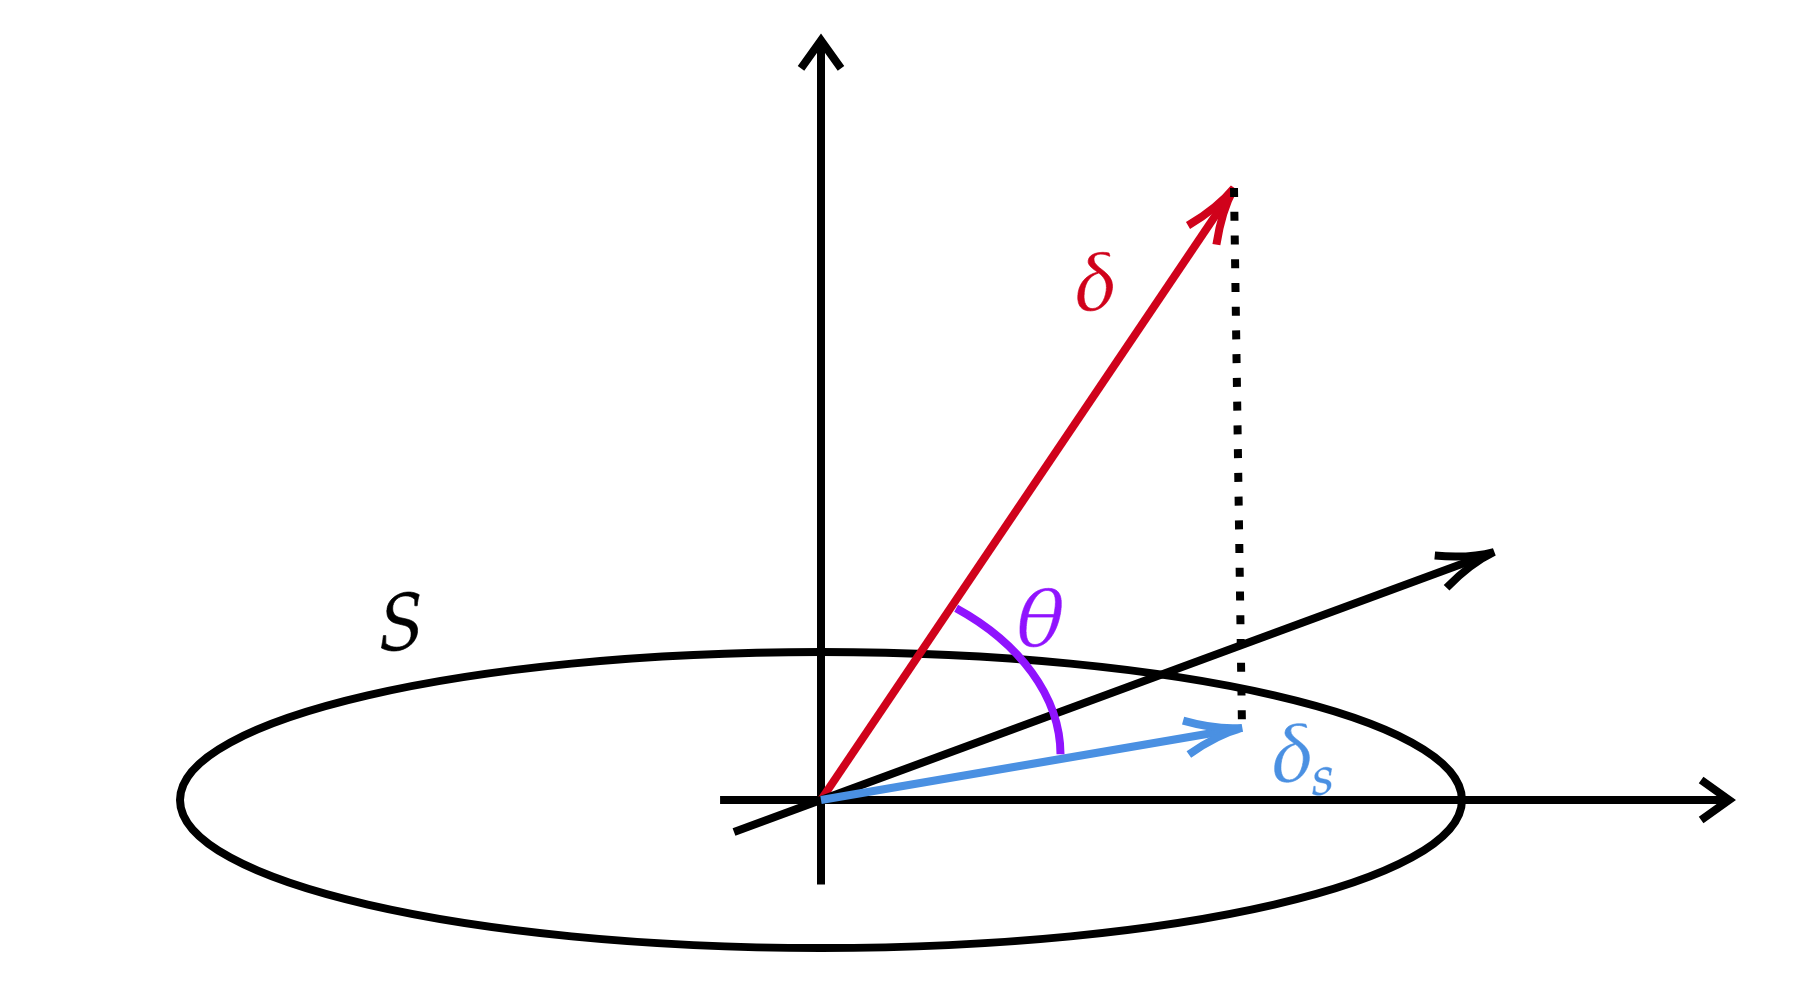
\includegraphics[scale=0.27]{mhous/plots/subspace_diag.png}
    \caption{\small Schematic representation of the geometric relation
      between the shift vector, $\delta\in D$, (here drawn as 3d), and
      the component, $\delta^S$, of the shift vector which lies in the 
subspace, $S$ (here drawn as 2d), containing the ellipse, $E$, defined by the theory covariance matrix. The angle $\theta$ between $\delta$ and $\delta^S$ is also shown; the dotted line shows the other side of the triangle, $\delta^{\rm miss}\in D/S$.
    \label{fig:subspace_diagram} }
  \end{center}
\end{figure}
%%%%%%%%%%%%%%%%%%%%%%%%%%%%%%%%%%%%%%%%%%%%%%%%%%%%%%%%%%%%%%%%%%%%%%%%%%%%%%%%%%%%%%%%%%%%%%%
Now that we have determined a suitable subspace, we can project the shift, $\delta_i$, onto these eigenvectors:
\be
\delta^\alpha = \sum_i \delta_i e_i^\alpha.
\ee
For a reasonable covariance matrix, $\delta^\alpha$ should be a similar size to $E$ in each dimension. We can then find the total component of the shift in $S$, 
\be
\delta_i^S = \sum_\alpha \delta^\alpha e_i^\alpha,
\ee
and the complementary component in the remaining space, $D/S$,
\be 
\delta_i^{miss} = \delta_i - \delta_i^S.
\ee
The validation will be a success if most of $\delta$ is in $S$, i.e. $|\delta_i^{miss}| \ll |\delta_i|$. Fig.~\ref{fig:subspace_diagram} depicts the relationship between these objects. Note that $\delta$, $\delta^S$ and $\delta^{miss}$ make up a right angled triangle, with some angle, $\theta$, between $\delta$ and $\delta^S$. For a successful validation, $\theta$ should be ``small".  Although there is no distinct cut-off of values here, note that given the dimension of $D$ is 100 times larger than $S$, for a random covariance matrix we would expect $\theta$ very close to 90$\degree$.

\subsection{Results of validation tests}
We now apply the validation tests outlined thus far to the NLO theory covariance matrices for the various prescriptions.

A first check can be done by comparing the diagonal elements, $\sigma_i$ where $\widehat{S}_{ii} = (\sigma_i)^2$, with the shifts, $\delta_i$. This tests whether the per-point uncertainties encompass the NLO to NNLO shift. In Fig.~\ref{fig:diag_shift_validation_asymmetric}, these comparisons are shown for all the prescriptions. Clearly, the shape of the MHOU is similar to the shape of the shift for the majority of the data and for each prescription. In fact, there is little difference between the prescriptions, except for the size of the uncertainty; 5-point is the least conservative and $\overline{5}$-point is the most conservative. From this we can see that the theory covmat is qualitatively descriptive of the observed higher order shift, in terms of size and correlation. We also note that the majority of the influence of prescription choice is on the off-diagonal elements. The range of scale variation looks to be broadly appropriate, therefore, with the caveat that for some points the MHOU is overestimated (see in particular NC DIS). This is a conservative treatment, however it could affect the weighting of data sets adversely.
%%%%%%%%%%%%%%%%%%%%%%%%%%%%%%%%%%%%%%%%%%%%%%%%%%%%%%%%%%%%%%%%%%%%%
\begin{figure}[H]
  \begin{center}
      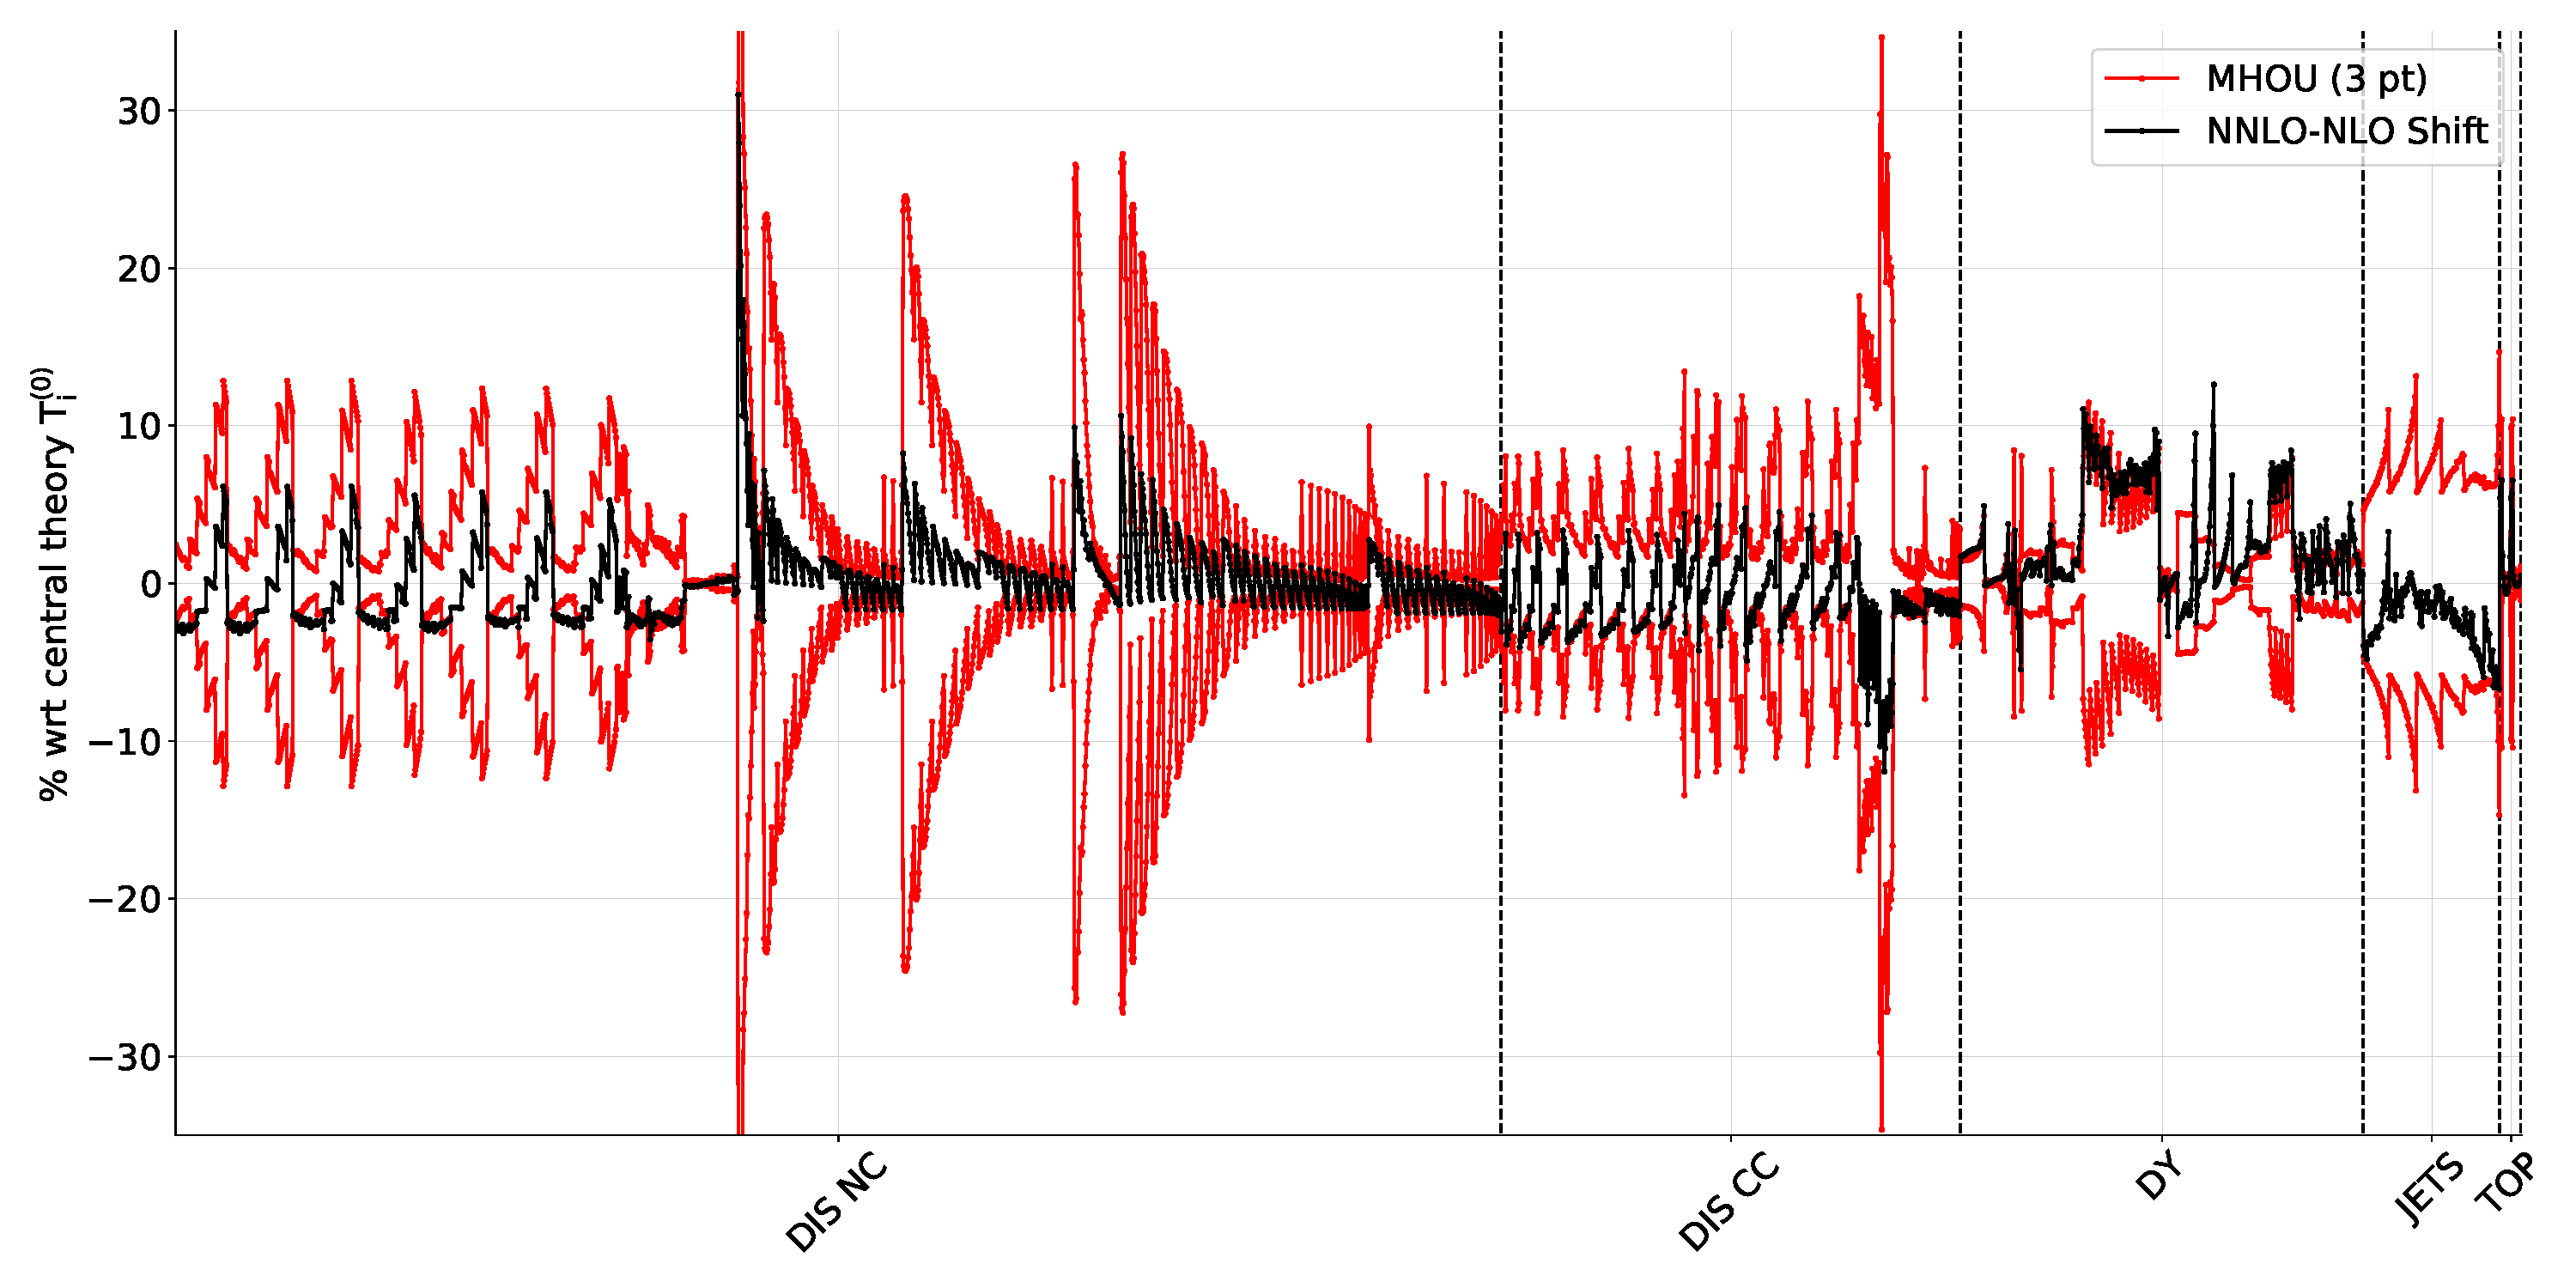
\includegraphics[width=14cm, height=4.3cm]{mhous/plots/shift_diag_cov_comparison_3pt_global.pdf}
    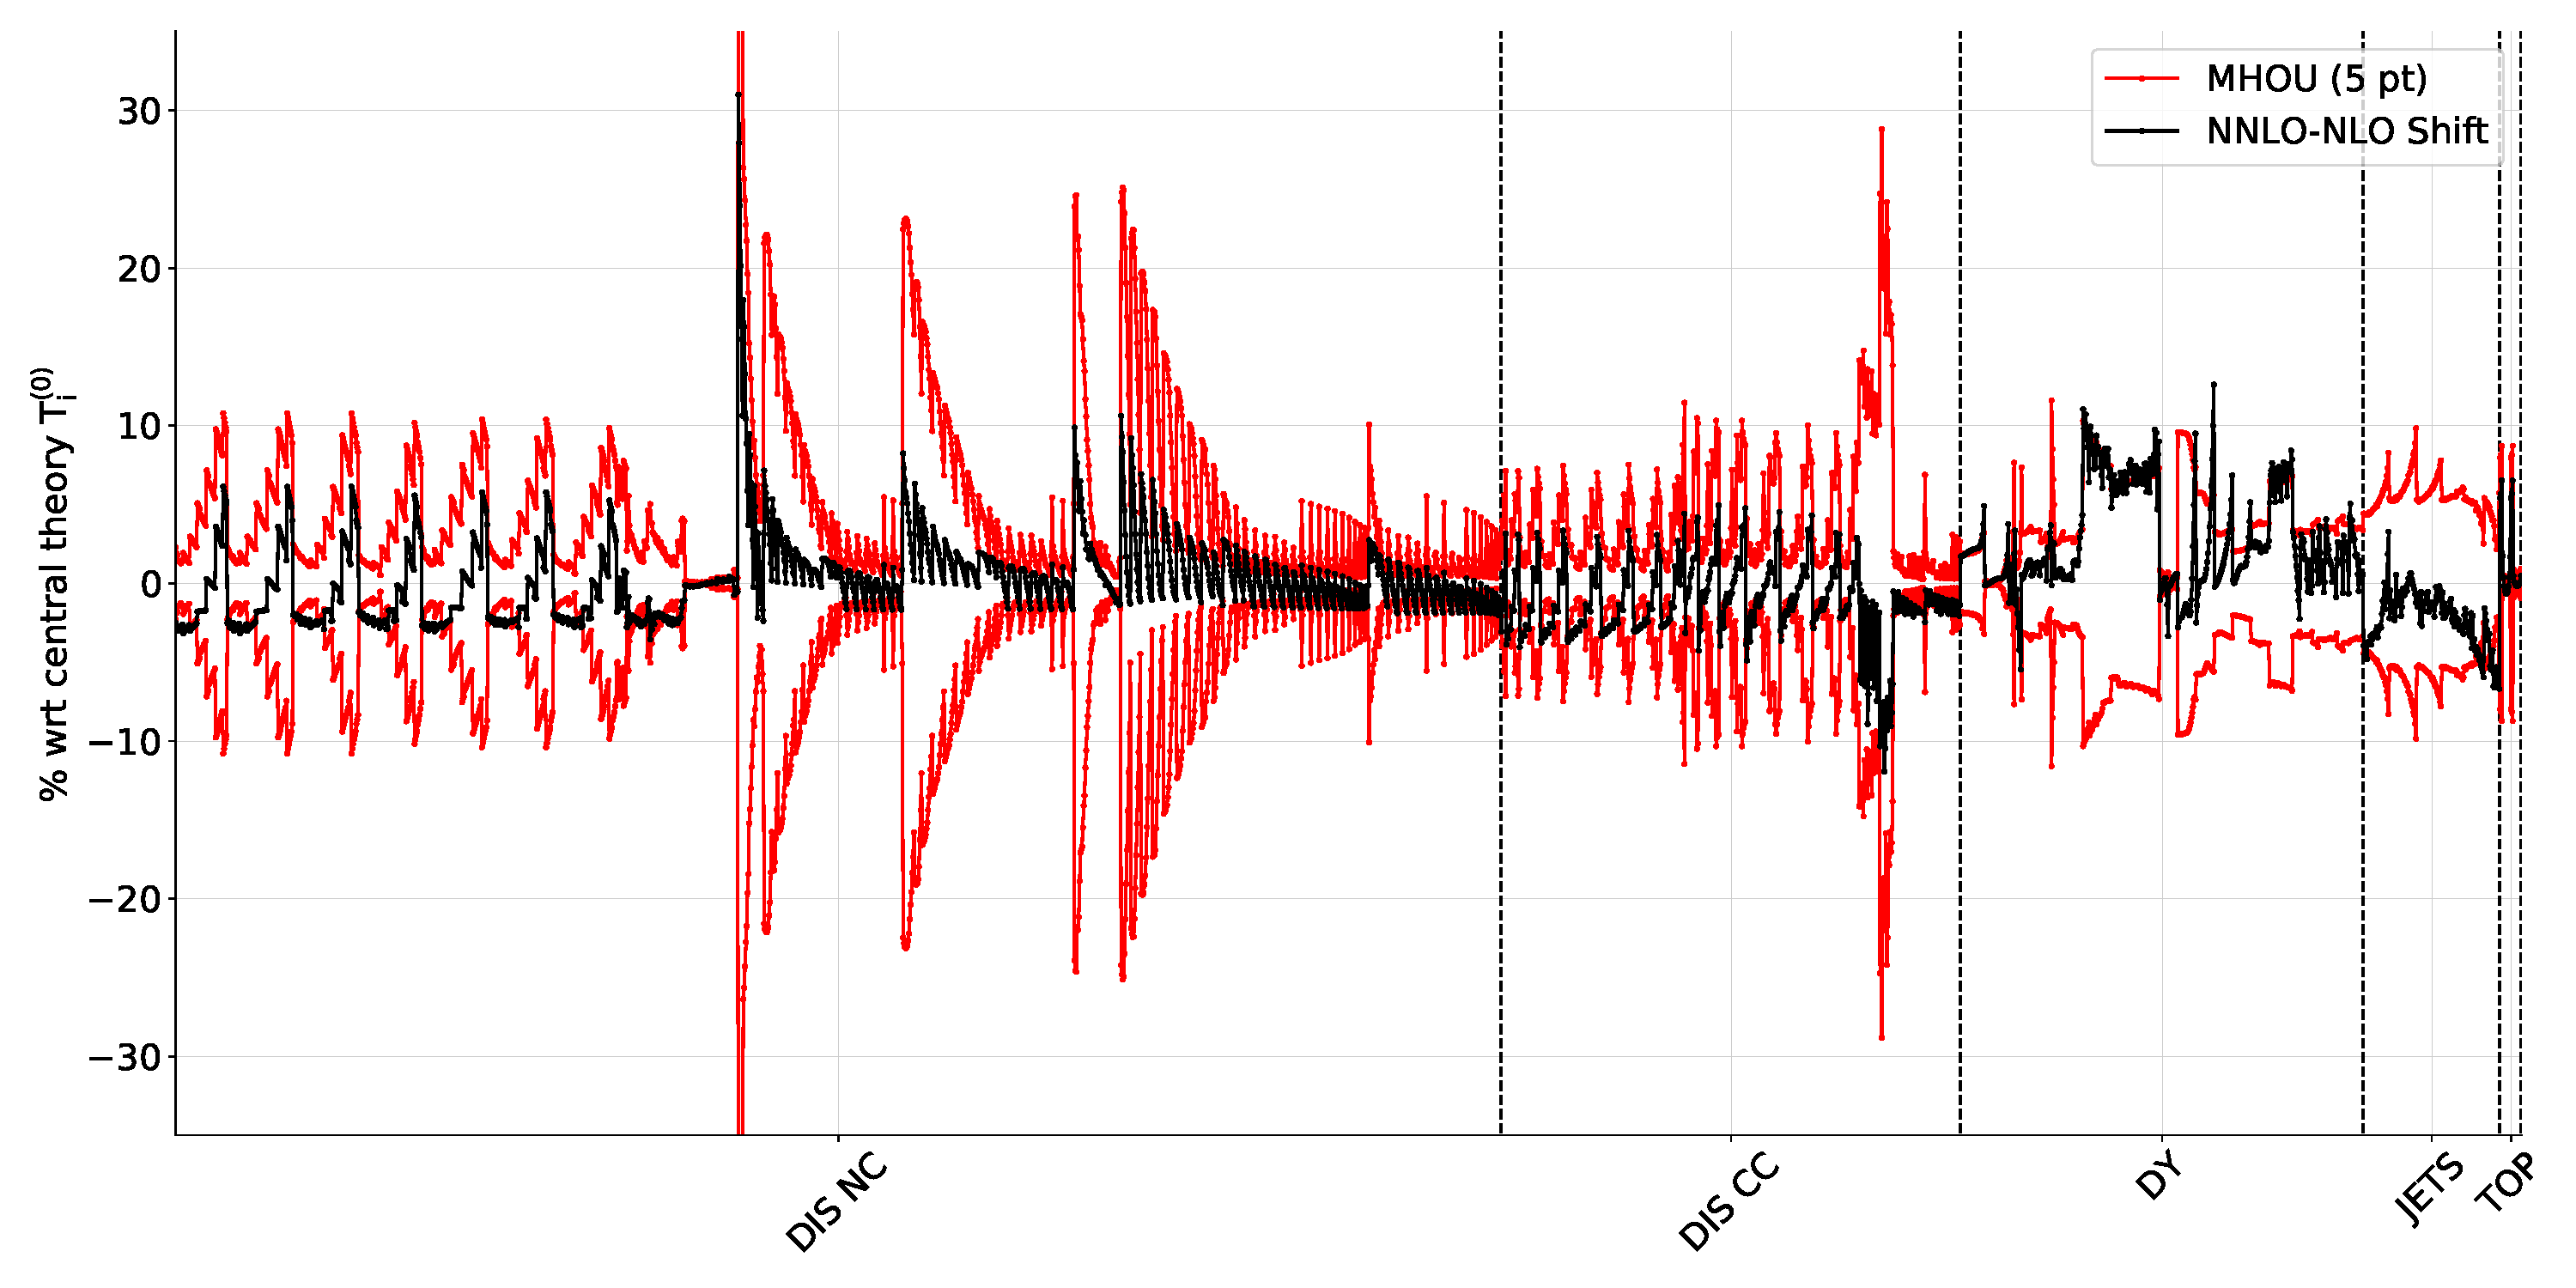
\includegraphics[width=14cm, height=4.3cm]{mhous/plots/shift_diag_cov_comparison_5pt_global.pdf}
    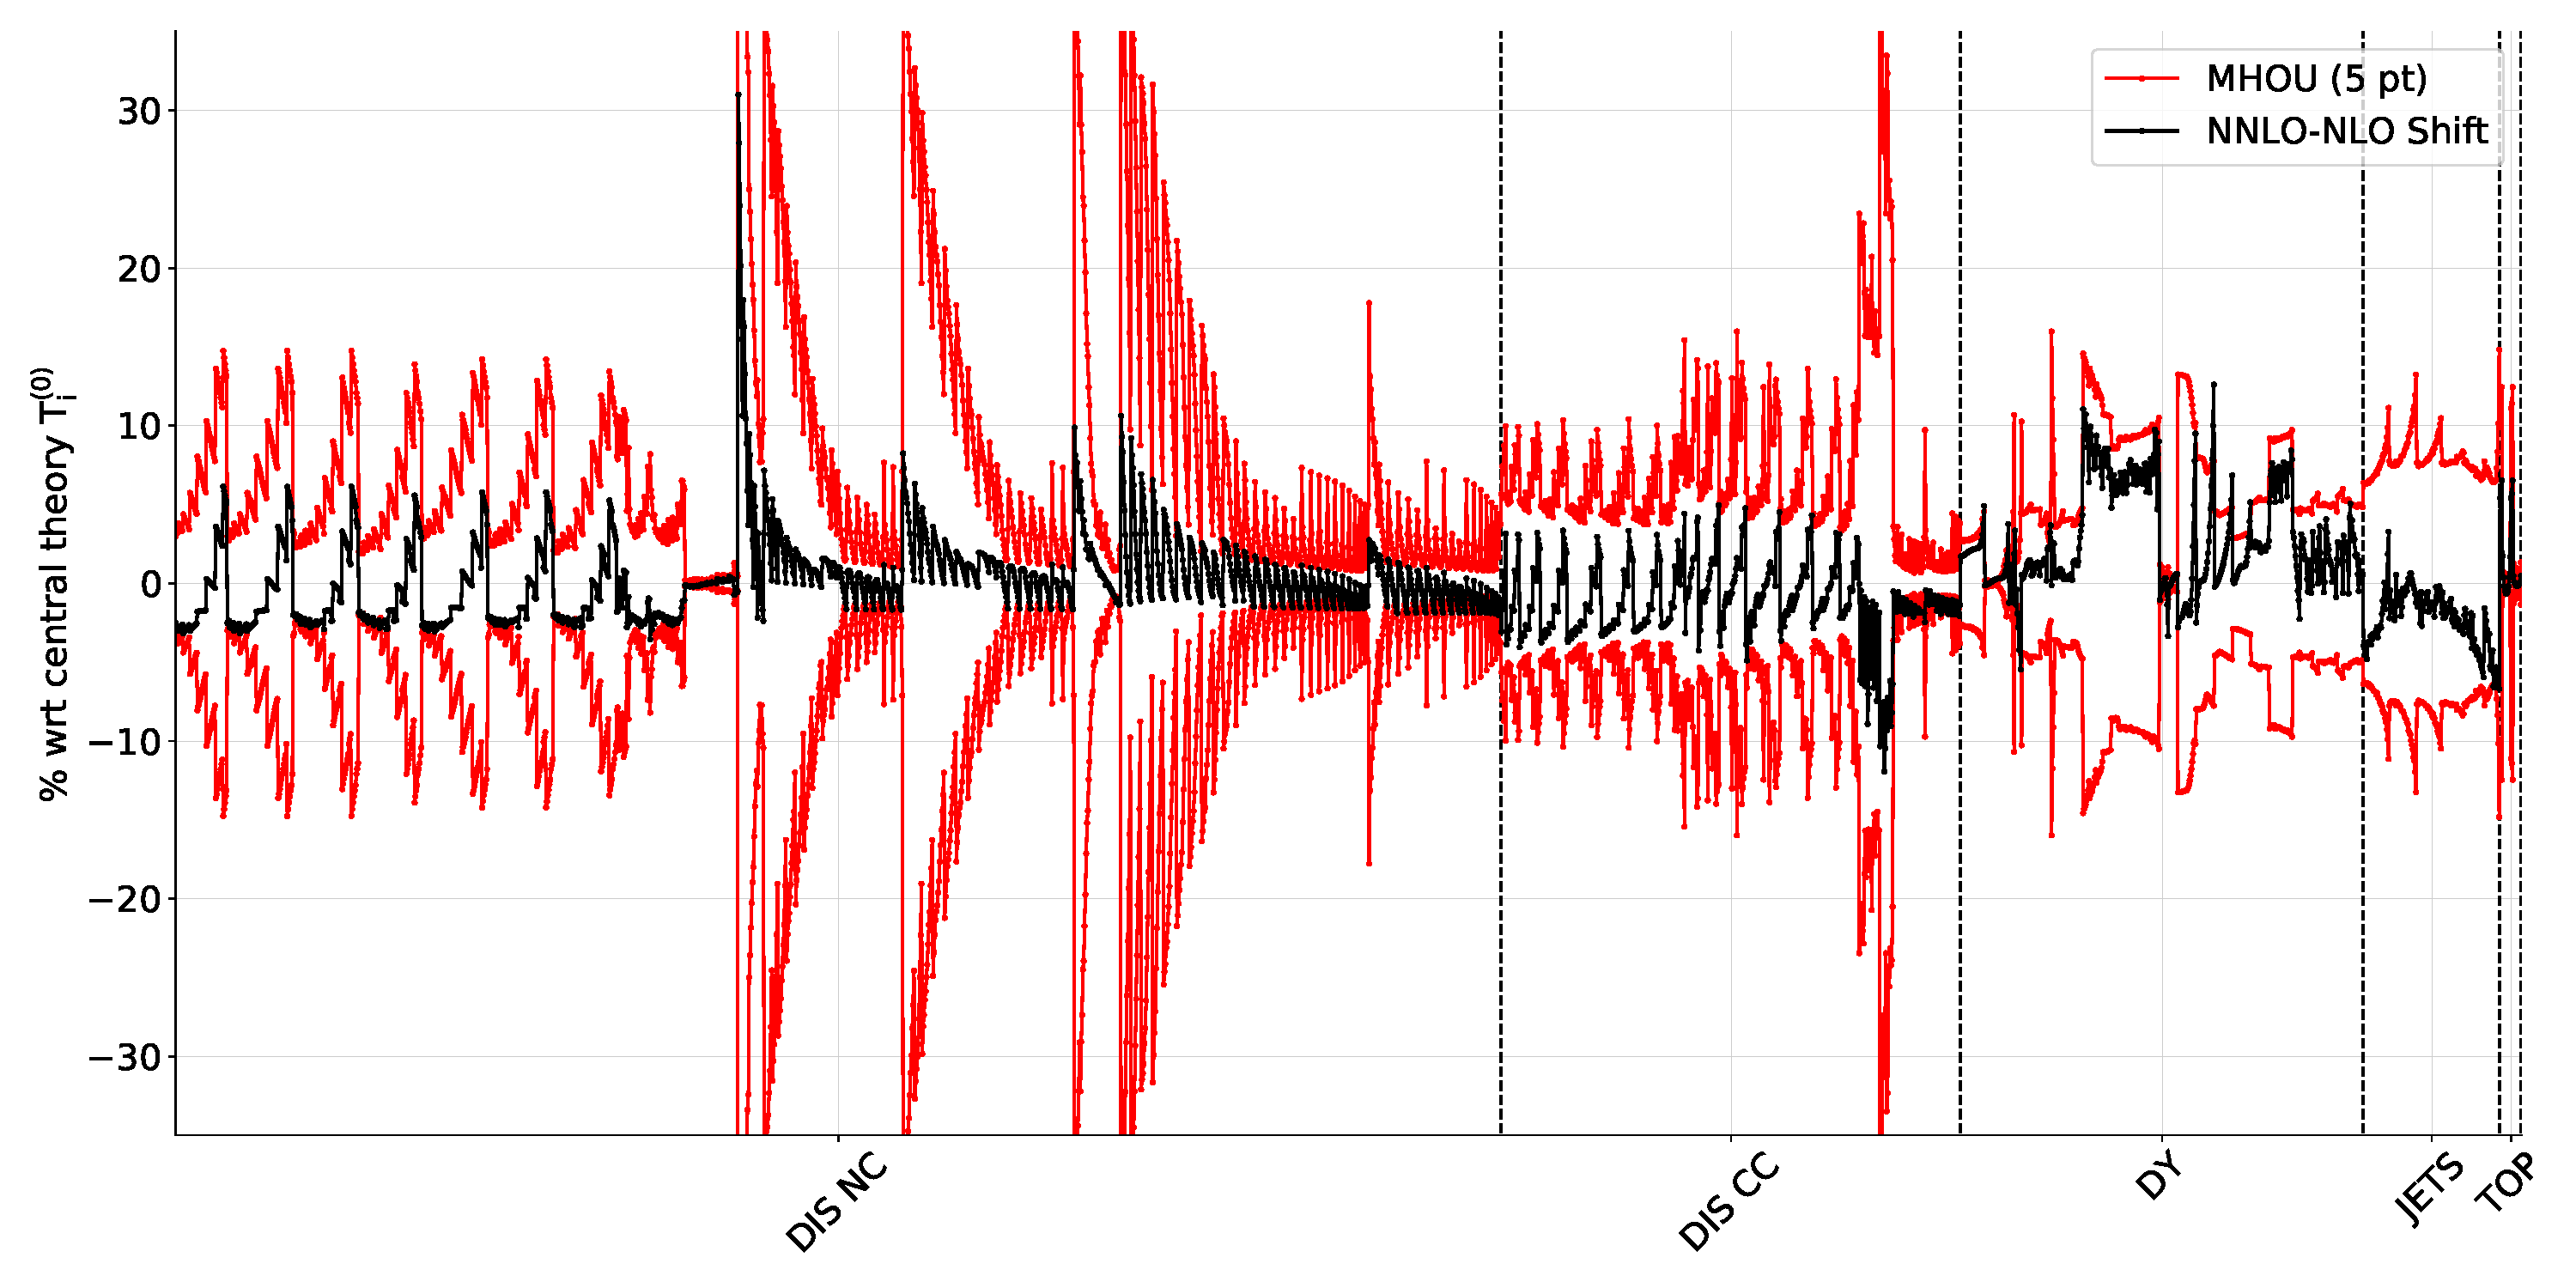
\includegraphics[width=14cm, height=4.3cm]{mhous/plots/shift_diag_cov_comparison_5barpt_global.pdf}
    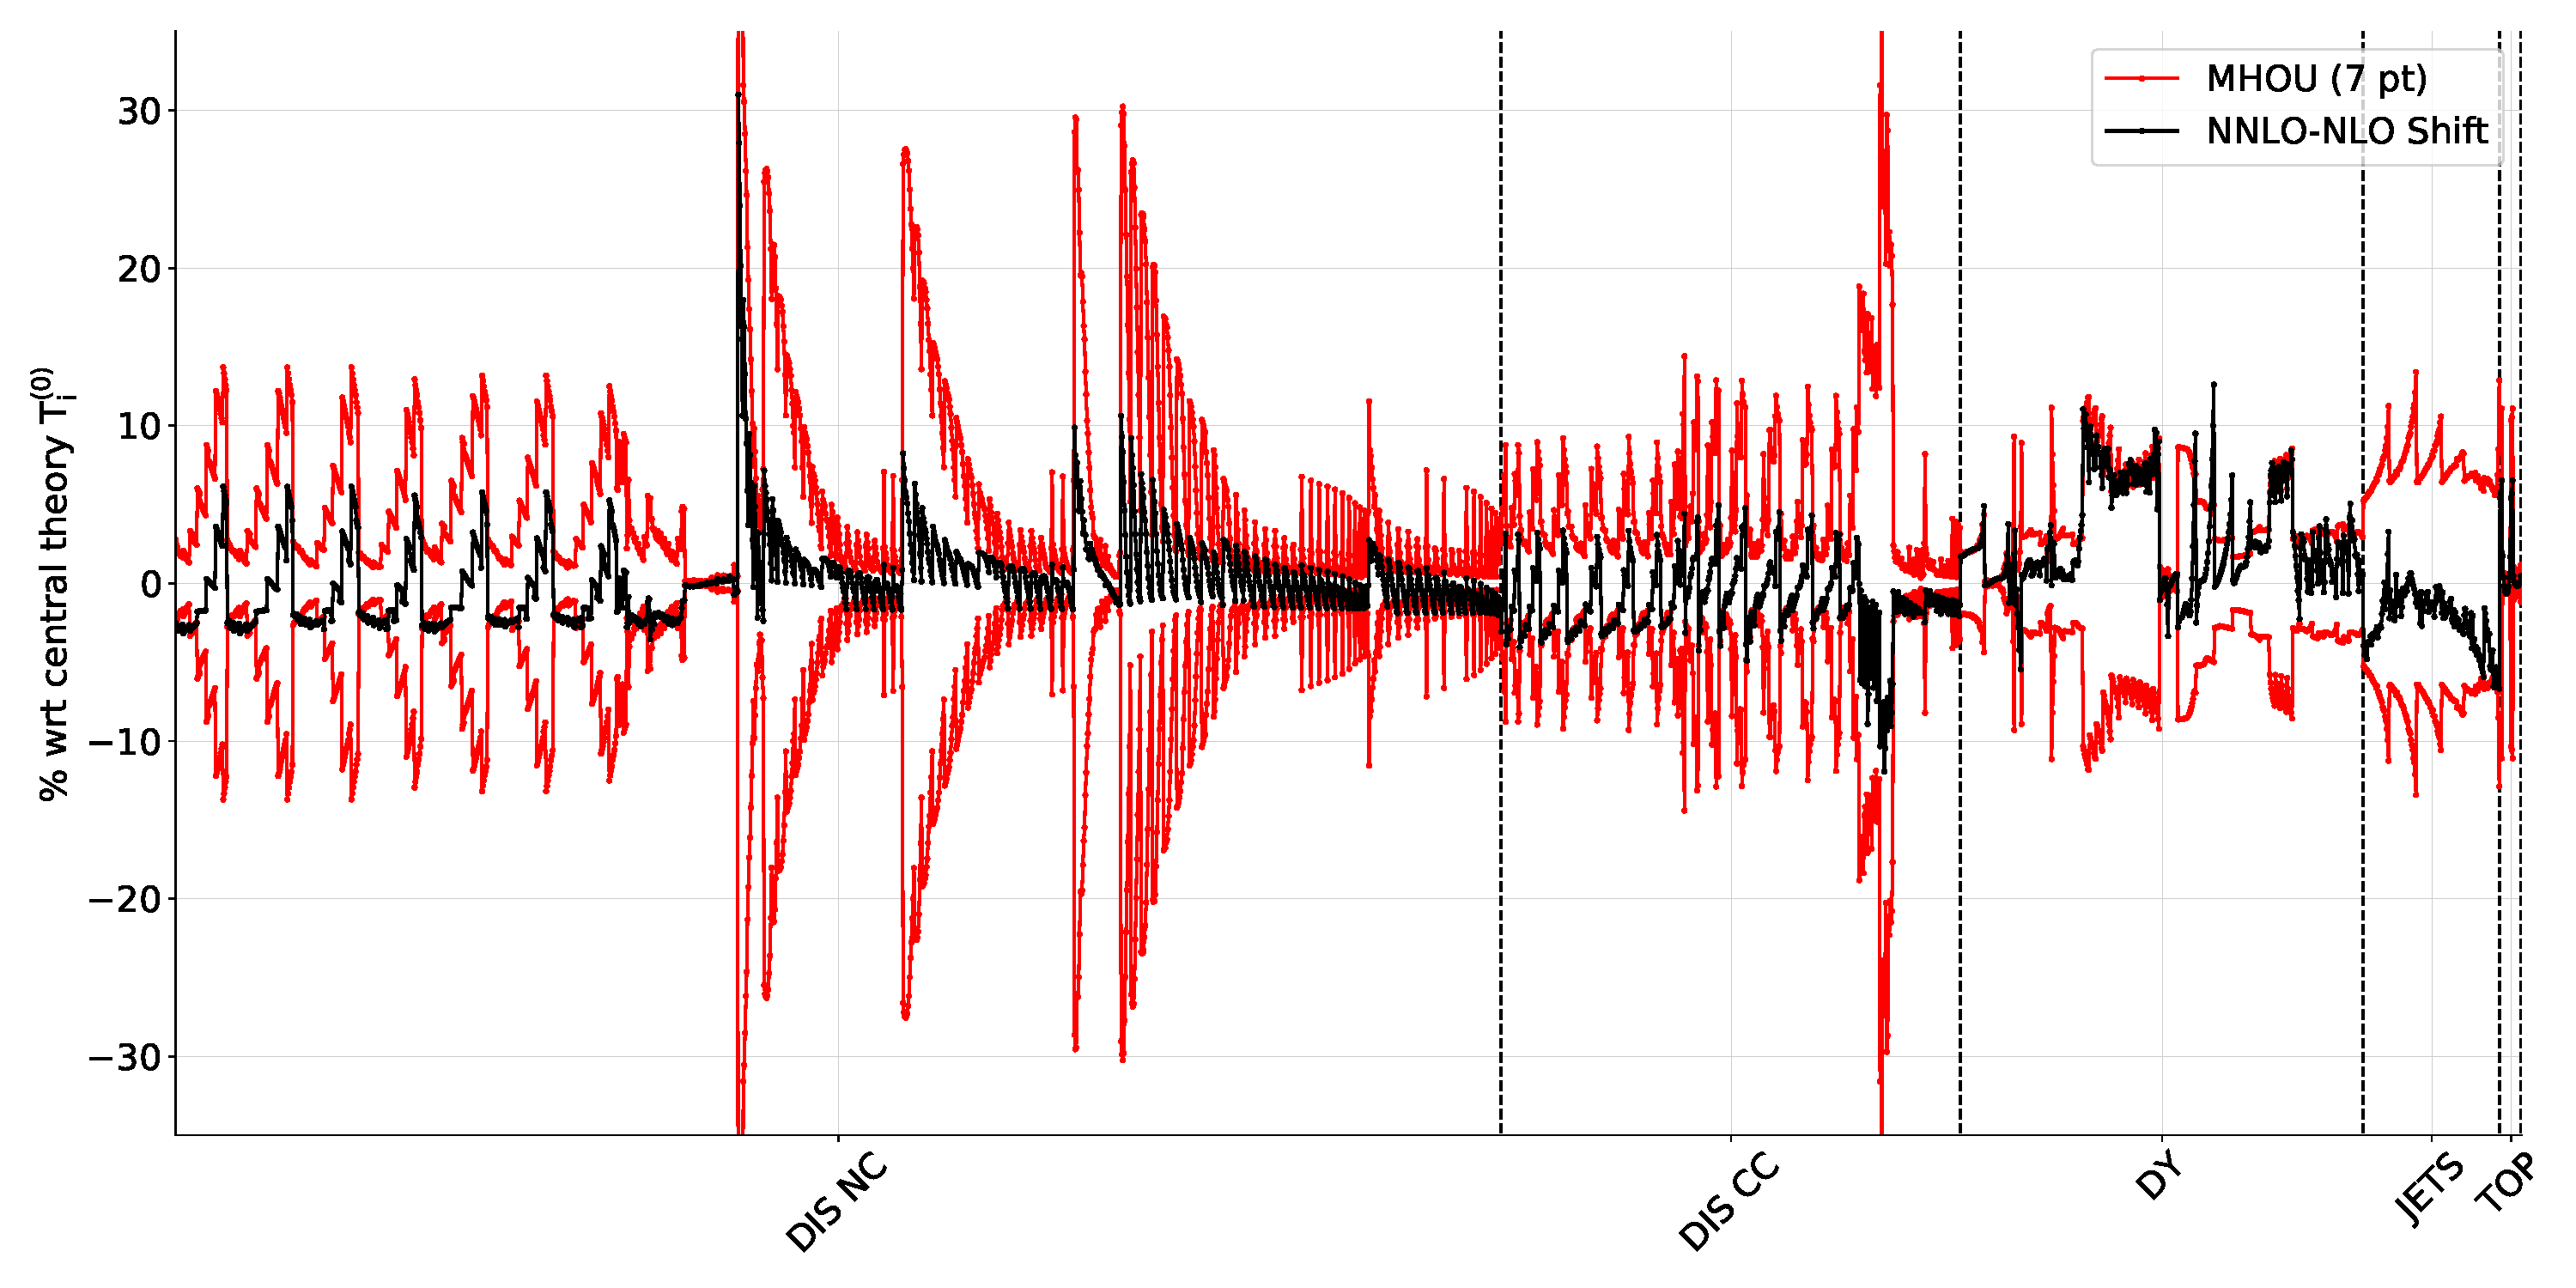
\includegraphics[width=14cm, height=4.3cm]{mhous/plots/shift_diag_cov_comparison_7pt_global.pdf}
    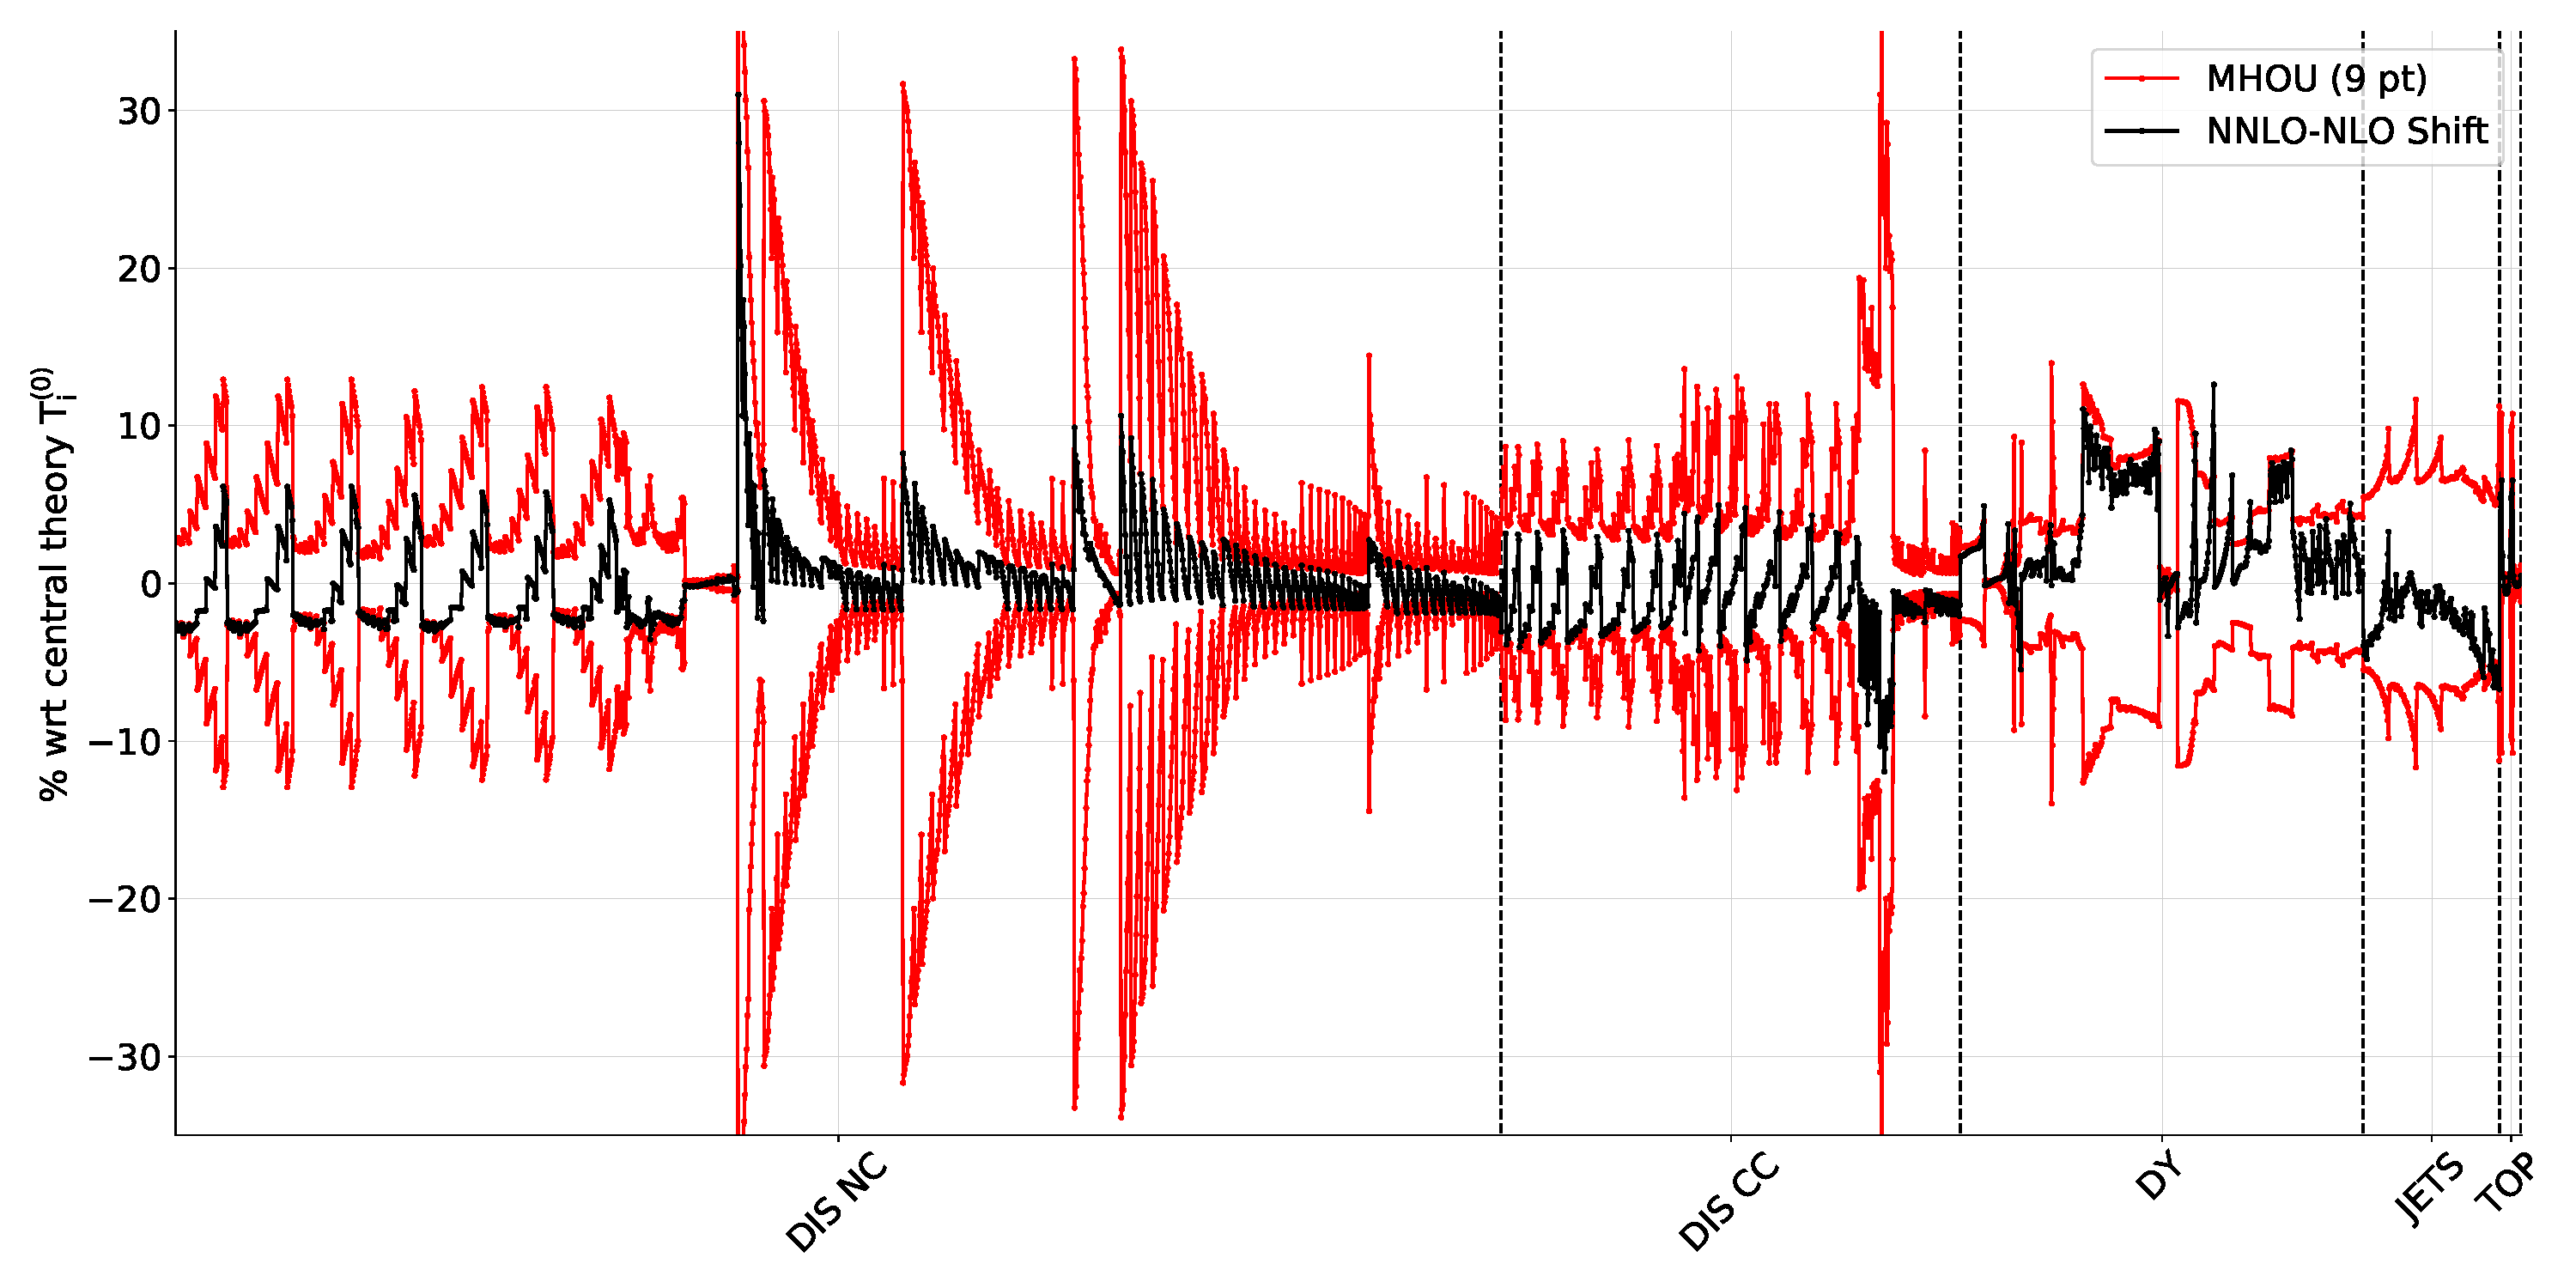
\includegraphics[width=14cm, height=4.3cm]{mhous/plots/shift_diag_cov_comparison_9pt_global.pdf}
    \caption{\small The diagonal uncertainties  $\sigma_i$ (red)
      symmetrized about zero,
      compared to the shift $\delta_i$ for each
      datapoint (black), for the prescriptions. From top to bottom: 3-point, 5-point
      $\overline{5}$-point, 7-point and 9-point (bottom). All values
      are shown as percentage of the central theory prediction.}
    \label{fig:diag_shift_validation_asymmetric}
  \end{center}
\end{figure}
%%%%%%%%%%%%%%%%%%%%%%%%%%%%%%%%%%%%%%%%%%%%%%%%%%%%%%%%%%%%%%%%%%%%%%
To examine the efficacy of the correlations, we must turn to the methods discussed in the previous section. We first look at the angle, $\theta$, between the shift and its component in the subspace, $S$, spanned by the theory covariance matrix. 
%%%%%%%%%%%%%%%%%%%%%%%%%%%%%%%%%%%%%%%%%%%%%%%%%%%%%%%%%%%%%%%%%%%%%
\begin{table}[H]
	\centering
	%%%%%%%%%%%%%%%%%%%%%%%%%%%%%%%%%%%%%%%%%%%%%%%%%%%%%%%%%%%
\renewcommand*{\arraystretch}{1.30}
 \centering
\begin{tabular}{ccC{30pt}}
  \toprule
Prescription & $N_{\rm sub}$ & $\theta$ \\
\midrule
    5-pt & 8 & 33$^{\rm o}$ \\
    $\overline{5}$-pt & 12 & 31$^{\rm o}$ \\
    9-pt & 28 & 26$^{\rm o}$ \\\midrule
    3-pt & 6 & 52$^{\rm o}$ \\
    7-pt & 14 & 29$^{\rm o}$ \\
\bottomrule
\end{tabular}
%%%%%%%%%%%%%%%%%%%%%%%%%%%%%%%%%%%%%%%%%%%%%%%%%%%%%%%%

        \vspace{5mm}
	\caption{\small The angle, $\theta$, between the NNLO-NLO
          shift and its component, $\delta_i^S$, lying within the
          subspace $S$ (see Fig.~\ref{fig:subspace_diagram})
          spanned by the theory covariance matrix for  different
          prescriptions. The dimension of the subspace $S$ in each case
          is also given.}
	\label{tab:global_efficiencies}
\end{table}
%%%%%%%%%%%%%%%%%%%%%%%%%%%%%%%%%%%%%%%%%%%%%%%%%%%%%%%%%%%%%%%%%%%%%
Tab.~\ref{tab:global_efficiencies} displays these values for each of the prescriptions. All of these are reasonably small, given that $N_{sub} \ll N_{dat}$, but 9-point is the best, with $\theta = 26 \degree$, due to the more comprehensive structure of scale variations. 3-point is unsurprisingly, the worst, suggesting that lack of correlation in the factorisation scale misses important correlations in the universal PDF evolution.
%%%%%%%%%%%%%%%%%%%%%%%%%%%%%%%%%%%%%%%%%%%%%%%%%%%%%%%%%%%%%%%%%%%%%
\begin{table}[H]
	\centering
	\small
	%%%%%%%%%%%%%%%%%%%%%%%%%%%%%%%%%%%%%%%%%%%%%%%%%%%%%%%%%%%
\renewcommand*{\arraystretch}{1.20}
\begin{tabular}{|c|c|c|c|c|c|c|c|}
 \toprule
%\cline{3-7}
% \multicolumn{5}{c|}{$\theta$} \\
Presc. & $N_{\rm sub}$ & DIS NC & DIS CC & DY & JET & TOP \\
\cline{3-7}
& & 1593 & 552 & 484 & 164 & 26 \\
\hline
 5-pt & 4 &39$^{\rm o}$ & 21$^{\rm o}$ & 25$^{\rm o}$ & 17$^{\rm o}$ & 11$^{\rm o}$	\\
$\overline{5}$-pt & 4 & 38$^{\rm o}$ & 17$^{\rm o}$ & 23$^{\rm o}$	& 22$^{\rm o}$ & 10$^{\rm o}$ \\
9-pt & 8 & 32$^{\rm o}$ & 16$^{\rm o}$ & 22$^{\rm o}$ & 14$^{\rm o}$ & 3$^{\rm o}$	\\
\hline
 3-pt & 2 &54$^{\rm o}$ & 36$^{\rm o}$ & 39$^{\rm o}$ & 24$^{\rm o}$ & 12$^{\rm o}$ \\
7-pt & 6 &35$^{\rm o}$ & 17$^{\rm o}$ & 22$^{\rm o}$ & 16$^{\rm o}$ & 3$^{\rm o}$	\\
    \bottomrule
\end{tabular}
%%%%%%%%%%%%%%%%%%%%%%%%%%%%%%%%%%%%%%%%%%%%%%%%%%%%%%%%%%%%%%%%%%

        \vspace{3mm}
	\caption{Same as Table~\ref{tab:global_efficiencies}
          for each process of Table~\ref{tab:datasets_process_categorisation}. The number of data points in each process is given directly below the name of the process.}
	\label{tab:process_efficiencies}
\end{table}
%%%%%%%%%%%%%%%%%%%%%%%%%%%%%%%%%%%%%%%%%%%%%%%%%%%%%%%%%%%%%%%%%%%%%
Tab.~\ref{tab:process_efficiencies} shows the same analysis carried out individually for the various processes. The same hierarchy of prescriptions is evident within each process, with $\theta$ smallest for the processes with the least data (e.g. TOP). This is expected, since larger collections of data span a greater kinematic range and include a richer structure, which is correspondingly harder to capture. DIS NC, the largest process, is the most poorly described. Note that the global value for $\theta$ is better than this, and so it is correlations within individual processes which are hardest to capture.

Having established what fraction of $\delta_i$ falls within $S$, we now go on to look at the complimentary component which falls outside, $\delta_i^{miss}$. Fig.~\ref{fig:deltamiss} shows this alongside $\delta_i$. The missing element is non-zero for all processes, and with a shape following that of the shift. This suggests there could be a component of $\delta_i$ which is missing for most data points, pointing to a poor estimation of the MHOU in the PDFs, which is common to all data. A good candidate for this is that the factorisation scale variation, as mentioned before, is only approximate; it would be better to include a separate variation for each of the eigenvalues of evolution, e.g. to first order splitting up the singlet and non-singlet.
%%%%%%%%%%%%%%%%%%%%%%%%%%%%%%%%%%%%%%%%%%%%%%%%%%%%%%%%%%%%%%%%%%%%%
\begin{figure}[H]
  \begin{center}
    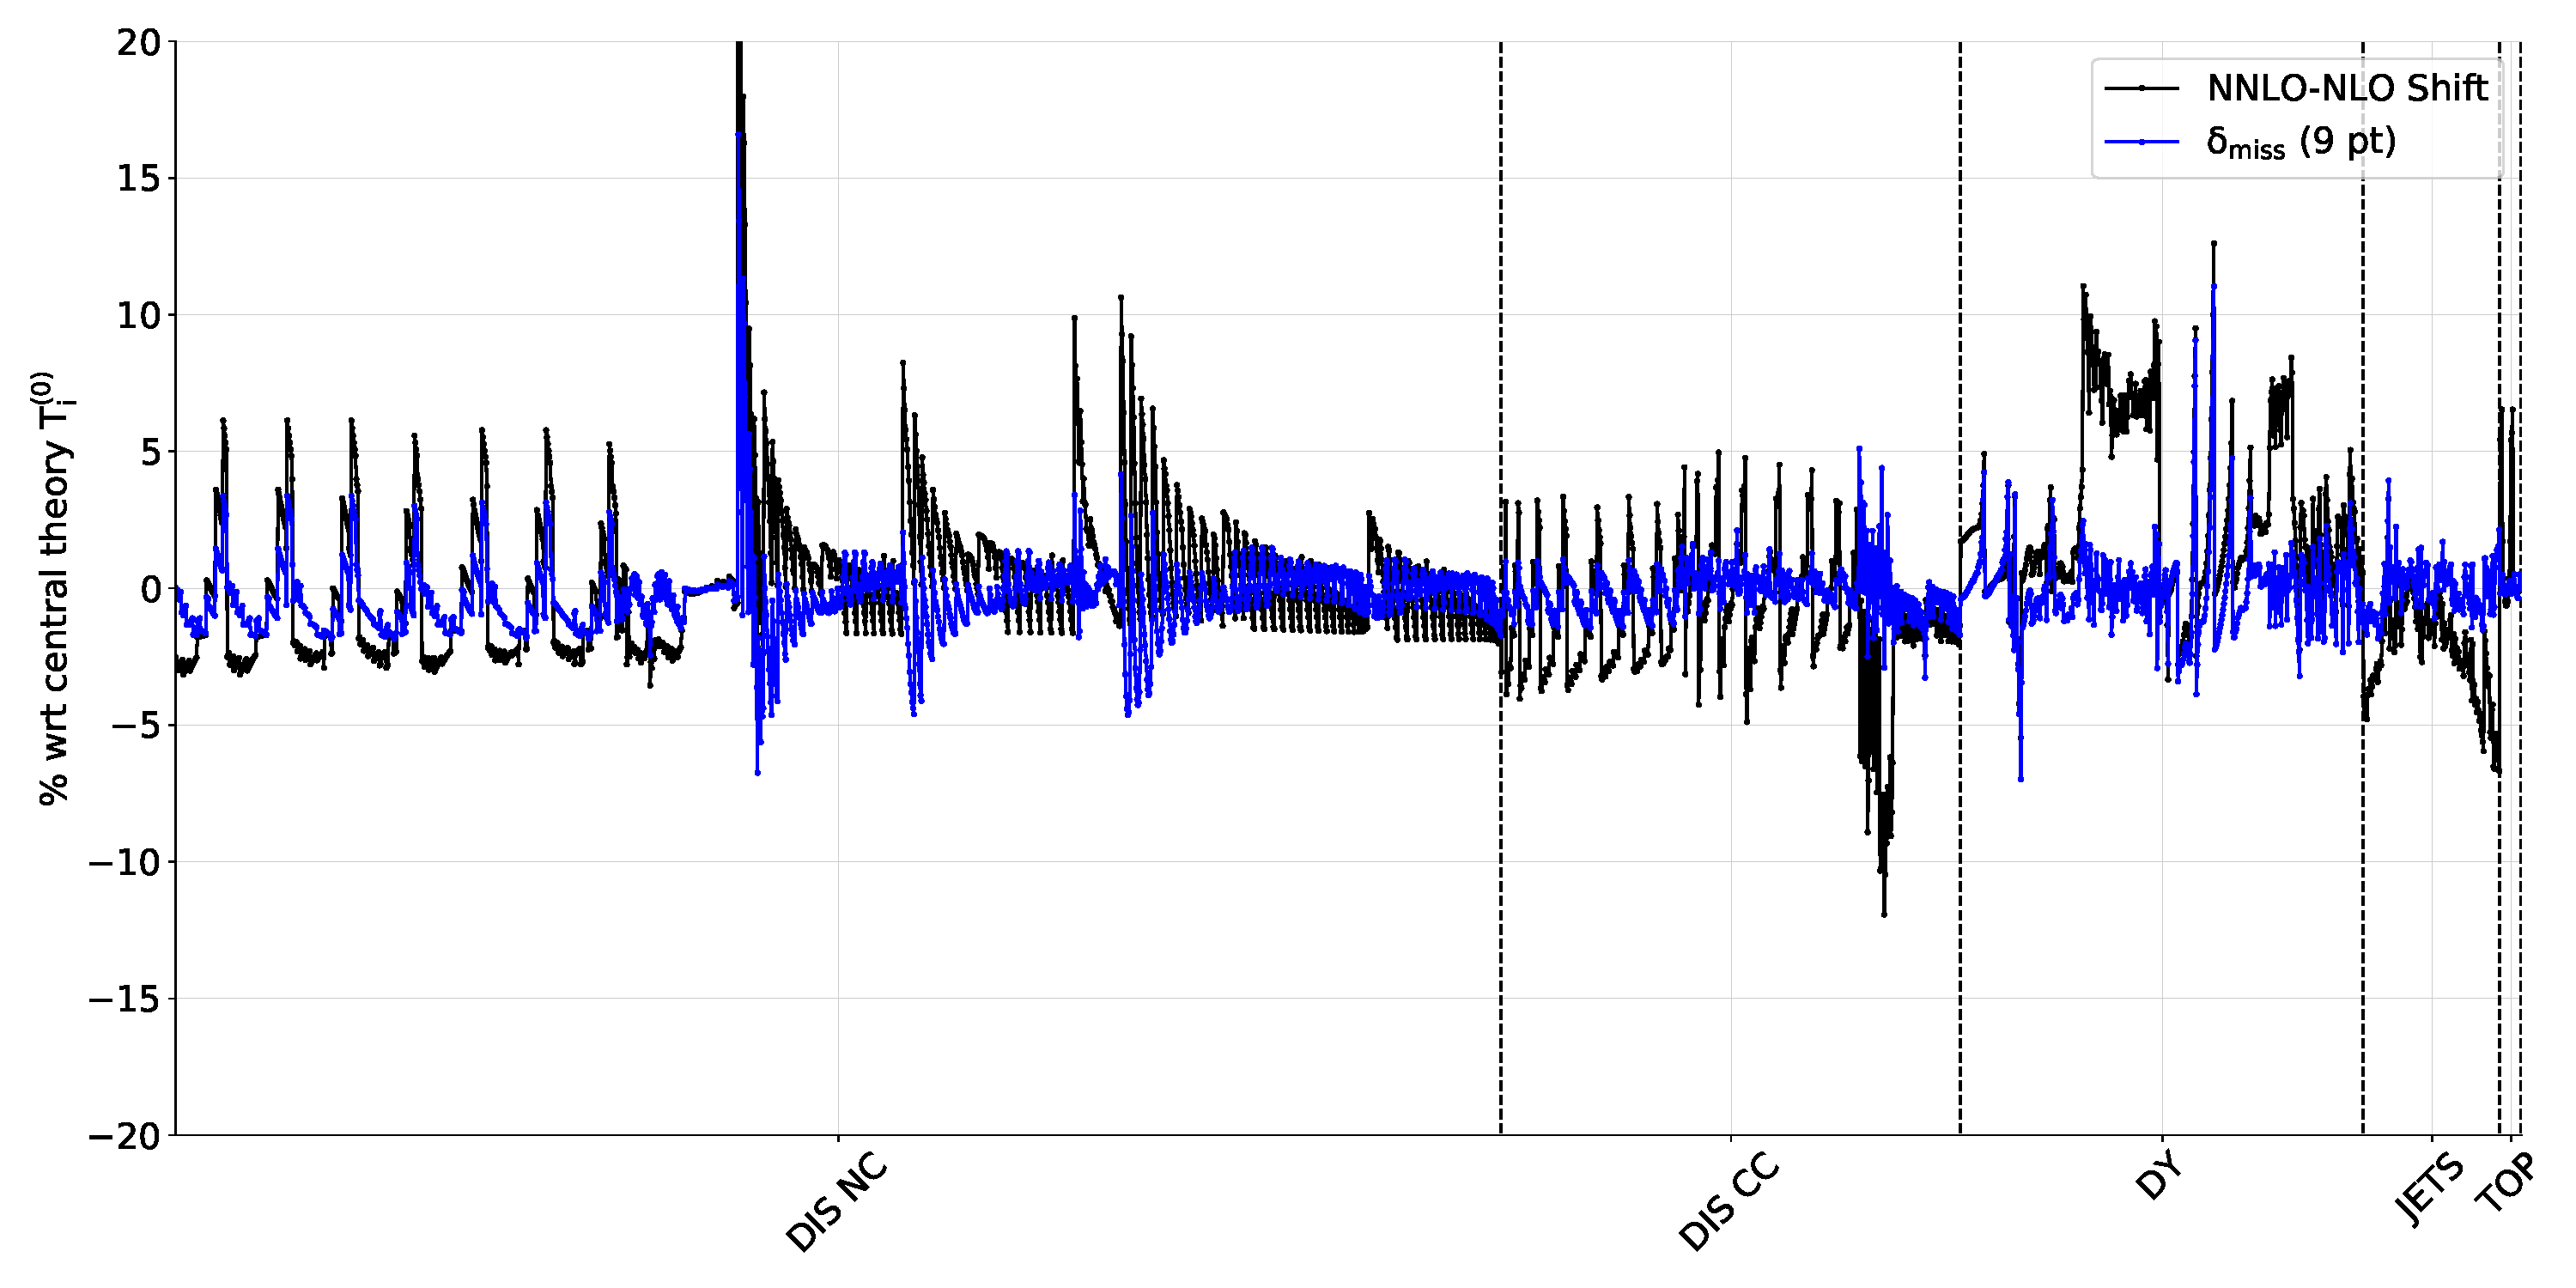
\includegraphics[width=0.99\textwidth]{mhous/plots/deltamiss_plot.pdf}
    \caption{The NNLO-NLO shift, $\delta_i$ (black), compared to its 
component, $\delta_i^{\rm miss}$ (blue), which lies outside the subspace $S$, computed using the 9-point prescription.}
    \label{fig:deltamiss}
  \end{center}
\end{figure}
%%%%%%%%%%%%%%%%%%%%%%%%%%%%%%%%%%%%%%%%%%%%%%%%%%%%%%%%%%%%%%%%%%%%%%

We know the component of the shift in the space of theory uncertainties, $S$, but we still need to see what fraction of this is encapsulated by the ellipse, $E$. To do this we look at the eigenvalues of the theory covariance matrix, $\lambda^\alpha = (s^\alpha)^2$. These are the lengths of the semi-axes of $E$, and there are as many as $N_{sub}$. We can compare them to $\delta^\alpha$, the projections of the shift onto each eigenvector. 
%%%%%%%%%%%%%%%%%%%%%%%%%%%%%%%%%%%%%%%%%%%%%%%%%%%%%%%%%%%%%%%%%%%%%%
\begin{figure}[H]
  \begin{center}
    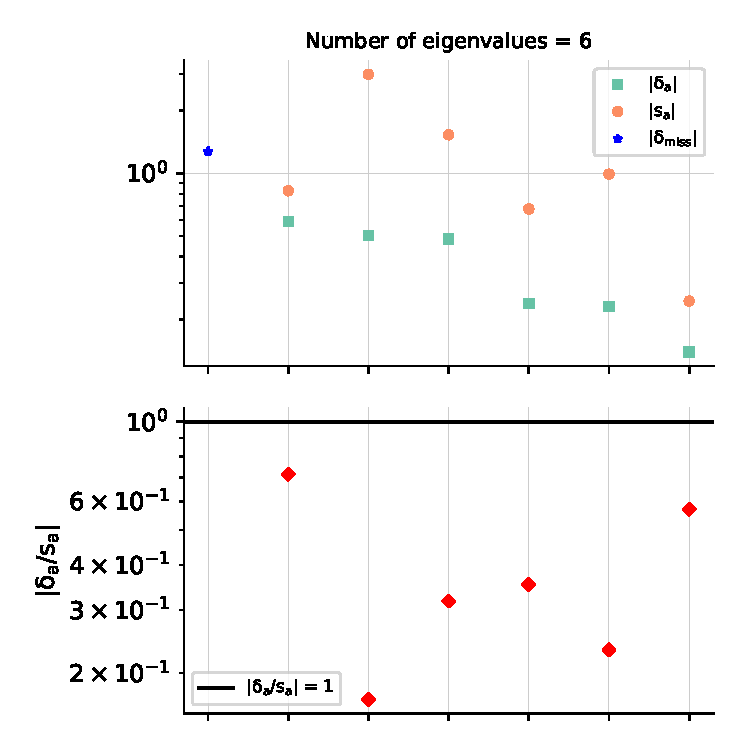
\includegraphics[scale=0.55]{mhous/plots/projector_eigenvalue_ratio_3pt_global.pdf}
    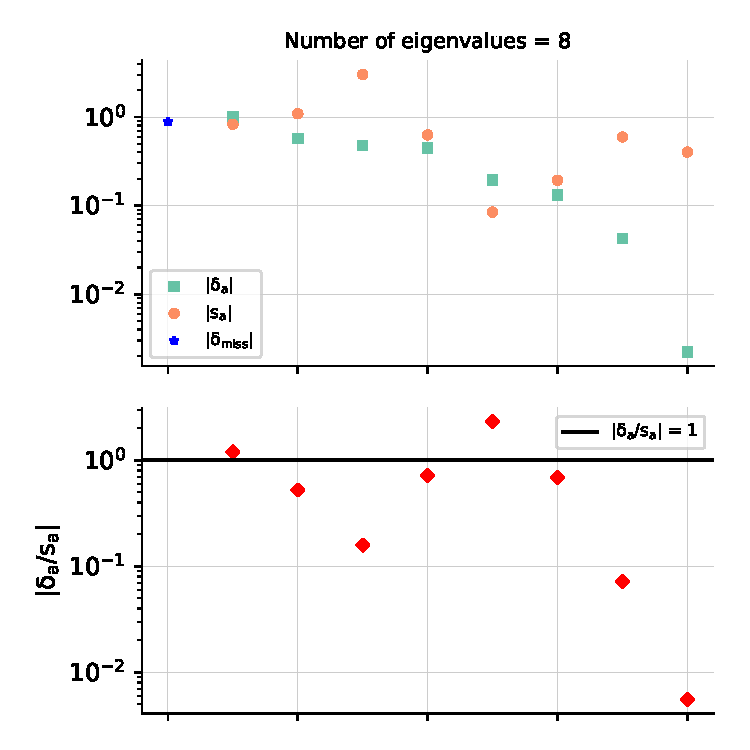
\includegraphics[scale=0.55]{mhous/plots/projector_eigenvalue_ratio_5pt_global.pdf}
    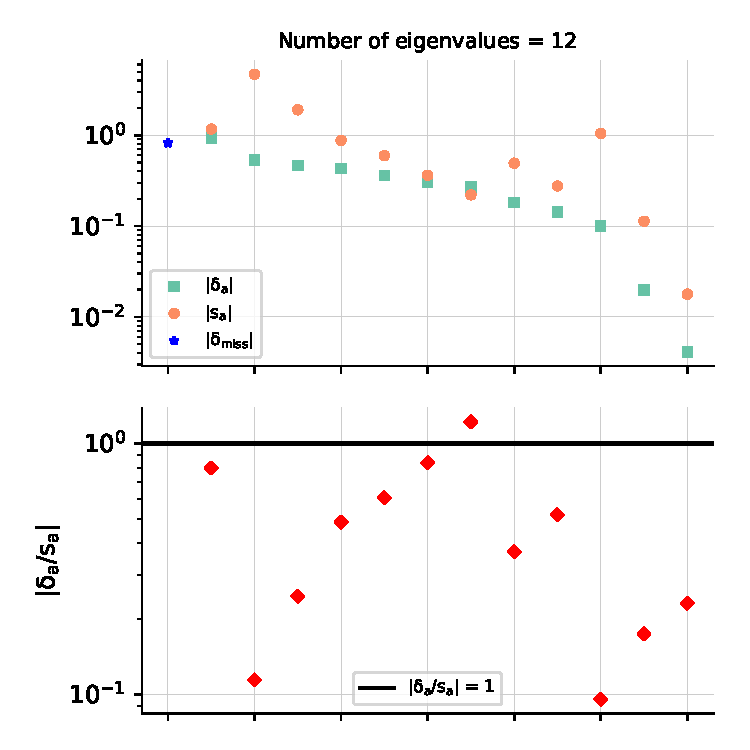
\includegraphics[scale=0.55]{mhous/plots/projector_eigenvalue_ratio_5barpt_global.pdf}
    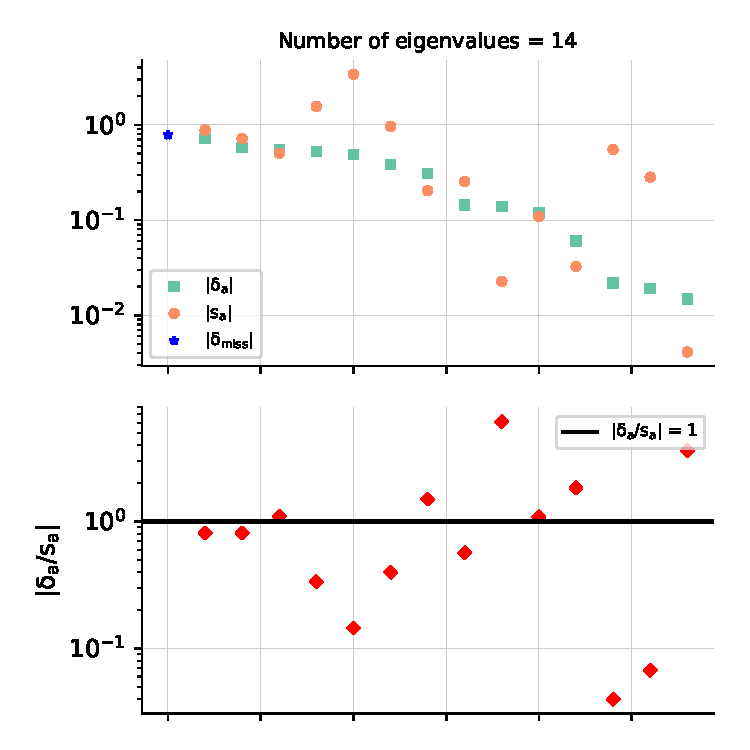
\includegraphics[scale=0.55]{mhous/plots/projector_eigenvalue_ratio_7pt_global.pdf}
    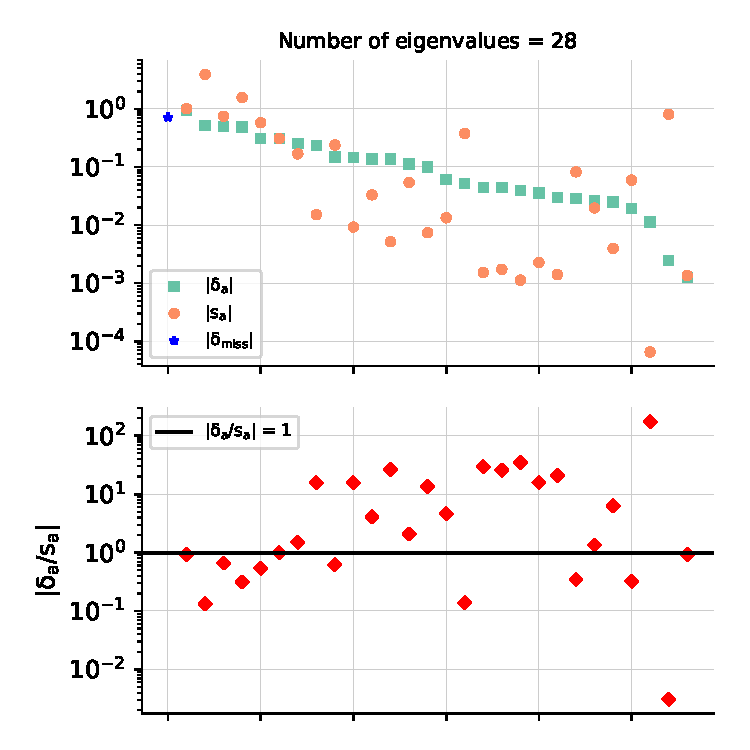
\includegraphics[scale=0.55]{mhous/plots/projector_eigenvalue_ratio_9pt_global.pdf}
    \caption{\small The projection, $\delta^\alpha$, of the normalised shift vector,
      $\delta_i$, along each eigenvector, $e^\alpha_i$, of $\Shat$, compared to the corresponding eigenvalue ,
    $s^\alpha$, ordered
      by the size of the projections (from largest to
      smallest). In each case results are shown as absolute (upper) and
      as ratios $\delta^\alpha/s^\alpha$ (lower). The magnitude of missing component, $|\delta^{\rm miss}_i|$ is also shown (blue star).
      Prescriptions: (top left) 3-point, 5-point
      $\overline{5}$-point, 7-point and 9-point (bottom right)}
        \label{fig:evals_all_prescriptions}
  \end{center}
\end{figure}
%%%%%%%%%%%%%%%%%%%%%%%%%%%%%%%%%%%%%%%%%%%%%%%%%%%%%%%%%%%
%%%%%%%%%%%%%%%%%%%%%%%%%%%%%%%%%%%%%%%%%%%%%%%%%%%%%%%%%%%%%%%%%%%%%%
\begin{figure}[H]
  \begin{center}
    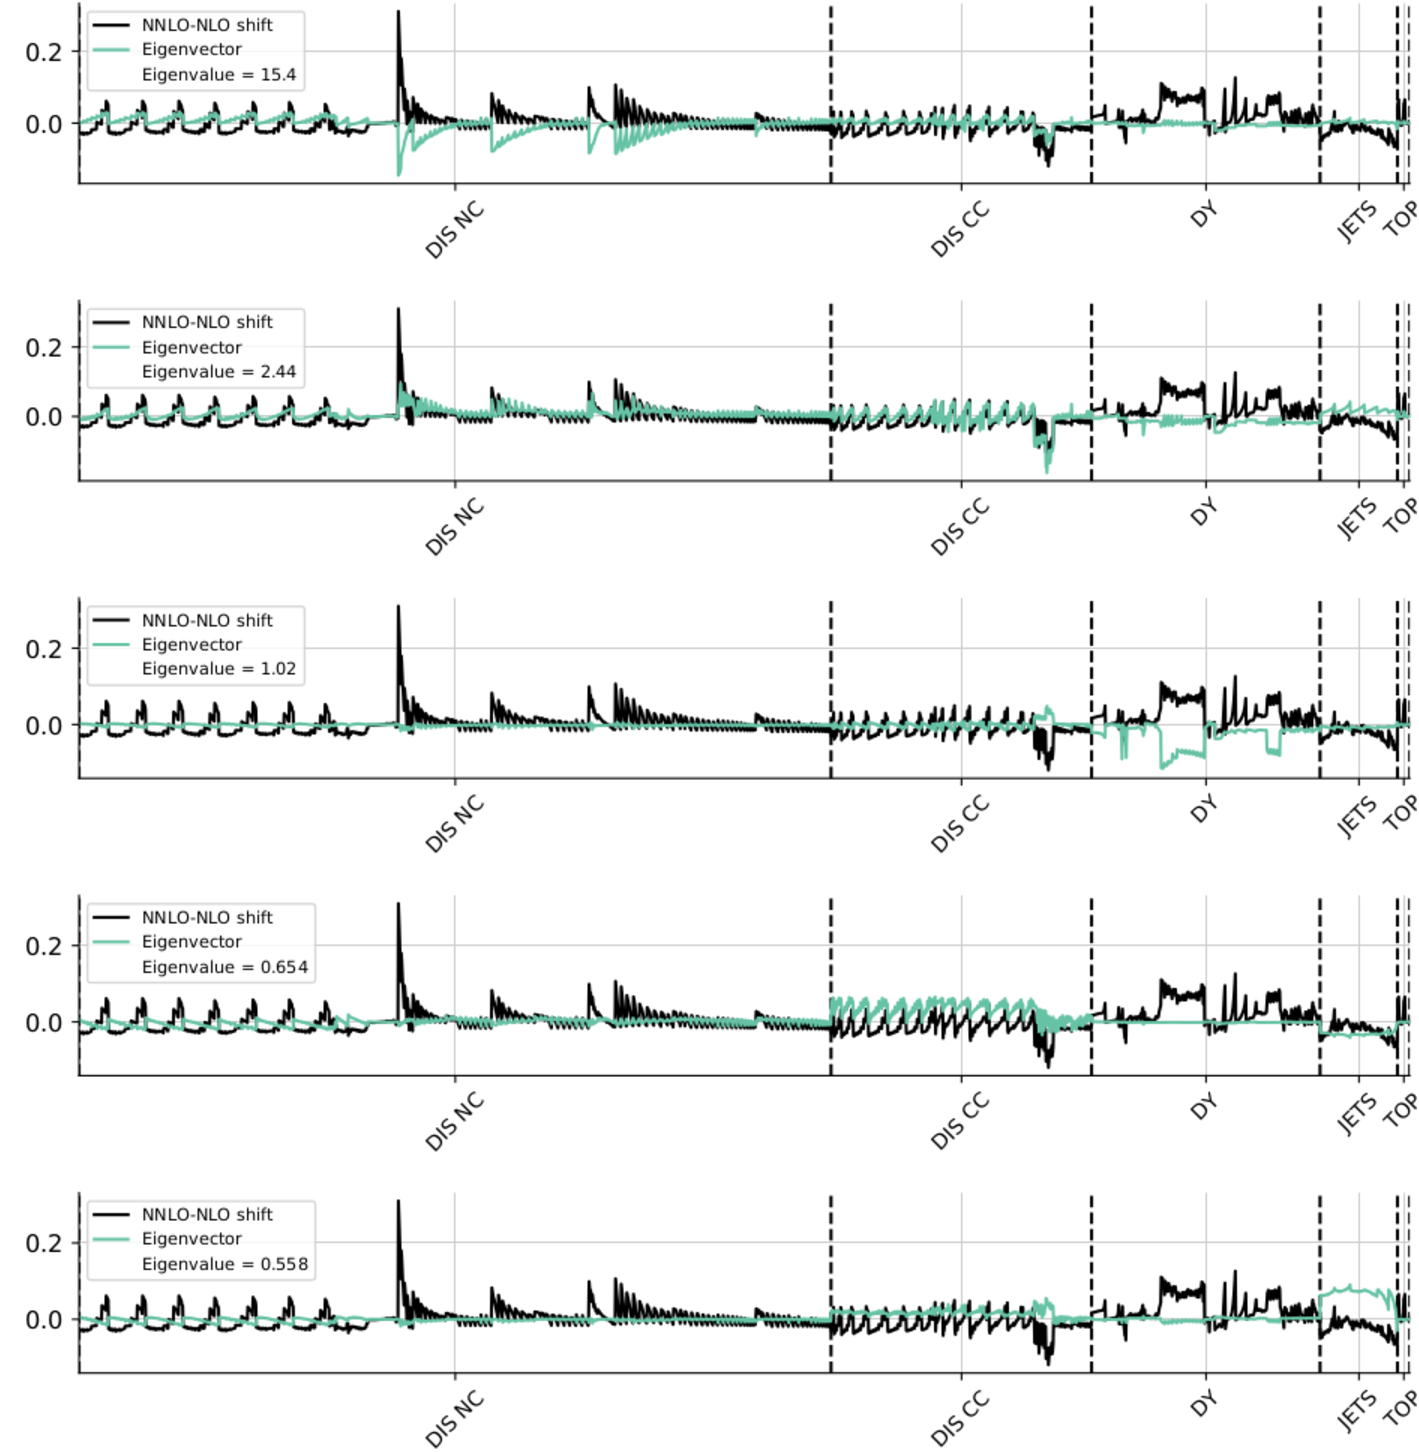
\includegraphics[width=0.95\textwidth]{mhous/plots/eigenvector_plot_10.pdf}\\
    \caption{\small The components,  $e^\alpha_i$ (green), of the eigenvectors, corresponding
      to the five largest eigenvalues for the 9-point theory covariance matrix. The NNLO-NLO shift, $\delta_i$ (black), is shown for comparison.
    \label{fig:evecs1} }
  \end{center}
\end{figure}
%%%%%%%%%%%%%%%%%%%%%%%%%%%%%%%%%%%%%%%%%%%%%%%%%%%%%%%%%%%%%%%%%%%%%%
Fig.~\ref{fig:evals_all_prescriptions} shows these values for each prescription. All the prescriptions do a reasonable job, in that the largest eigenvalue is similar to the projection of the shift in that direction. Additionally, the size of the eigenvalues tends to decrease as the shift in that direction decreases. As expected, 3-point overestimates the uncertainty, with $\delta^\alpha < s^\alpha$ for all eigenvalues. This is also the case for most of 5- and $\overline{5}$-point. However, for the more complicated 7- and 9-point there is a better estimation for the larger eigenvalues, although a high scatter and poor prediction for the smaller ones; note that this is a result of only six scales being varied, so there is limited information available. Additionally, the missing component is less than the largest projection for the symmetric prescriptions but is greater for the asymmetric prescriptions. This, once again, supports the adoption of a symmetric prescription.

Finally we investigate the components of the eigenvectors in the data space, $D$. The five largest of these for the 9-point are plotted in Fig.~\ref{fig:evecs1}, alongside $\delta$. Each of these can be identified with a component of the variation. From largest to smallest: 1 is largely DIS NC; 2 is a mixture of DIS NC and CC; 3 is DY; 4 is DIS CC; 5 is JETS. Unsurprisingly, the largest is dominated by the largest process, and so on, until the important TOP contribution appears at the (unshown) 9th eigenvector.

Overall, we have shown that all of the prescriptions capture most of the important features of the MHOs, and that 9-point does so the most accurately, given its more complex structure of scale variation. We therefore adopt 9-point as our chosen prescription, and proceed in the next section to include a 9-point theory covariance matrix in NLO PDF fits.


\section{PDFs with missing higher order uncertainties}
\label{sec:pdfs}
In this section we present the goal of this project: PDFs at NLO with the systematic inclusion of MHOUs. We compare NLO PDFs with and without MHOUs against the known NNLO PDFs, addressing the stability of the results to changes in prescription for the covariance matrix (9-pt vs 7-pt vs 3-pt). We break down the impact of MHOUs by including them separately in the Monte-Carlo sampling and the fitting. 

To recap, there are only two places in which a theory covariance matrix changes the PDF determination: 
\subsubsection{Sampling}
Recall from Chapter \ref{chapter:background} that Monte Carlo pseudodata replicas $D_i^{(k)}$, $k=1, \dots N_{rep}$, are generated such that their covariance gives the total covariance matrix:
\be 
\lim_{N_{rep} \to \infty} \frac{1}{N_{rep}(N_{rep}-1)} \sum_{k=1}^{N_{rep}} (D_i^{(k)}- \langle D_i \rangle)(D_j^{(k)}- \langle D_j \rangle) = C_{ij} + S_{ij},
\ee
where $\langle \dots \rangle$ denotes an average over replicas. 
\subsubsection{Fitting}
During fitting the $\chi^2$ is minimised, and this depends on $S_{ij}$ through the equation:
\be
\chi^2 = \frac{1}{N_{dat}} \sum_{i,j}^{N_{dat}} (D_i - T_i) (C+S)_{ij}^{-1}(D_j - T_j),
\ee
where $C_{ij}$ is the t0 covariance matrix to avoid d'Agostini bias~\cite{DAgostini:1993arp, Ball:2009qv}, as mentioned in Chapter \ref{chapter:background}.

We can assess the quality of the fit using this $\chi^2$ estimator alongside the $\phi$ estimator, defined as
\be 
\phi = \sqrt{ \langle \chi^2_{exp}[T_i] \rangle - \chi^2_{exp}[\langle T_i \rangle ] },
\ee
where $\chi^2_{exp}$ is evaluated using the (non-t0) experimental covariance matrix, $C_{ij}$. Following \cite{Ball:2014uwa}, this can be expressed as
\be 
\phi = \sqrt{ \frac{1}{N_{dat}} \sum_{i,j=1}^{N_{dat}} (C_{ij} + S_{ij})^{-1} X_{ij} },
\ee
where $X_{ij} = \langle T_i T_j \rangle - \langle T_i \rangle \langle T_j \rangle$ is the covariance matrix of theoretical predictions. This is a measure of the consistency of the data; if they are consistent, then they should combine to reduce the uncertainty and so $\phi \ll 1$. The result should be a factor of $r_{\phi}$ greater than when $S$ is not included, where
\be
r_{\phi} = \sqrt{1 + \frac{1}{N_{dat}} \sum_{i,j=1}^{N_{dat}} C_{ij}^{-1} S_{ij} }.
\ee
This means that if there were no other changes we would expect PDF uncertainties to increase by $r_{\phi}$ upon including MHOUs. 
The PDFs considered in this section are summarised in Table~\ref{tab:thcovmatFits}. NNLO PDFs with MHOUs are to
be determined in a future work. The $\phi$ and $\chi^2$ values
for these fits are shown in Tables~\ref{table:chi2table_covth_global_nlo}, \ref{table:phitable_covth_global_nlo}, broken down by process type and, for $\chi^2$ by dataset.
%%%%%%%%%%%%%%%%%%%%%%%%%%%%%%%%%%%%%%%%%%%%%%%%%%%%%%%%%
  %%%%%%%%%%%%%%%%%%%%%%%%%%%%%%%%%%%%%%%%%%%%%%%%%%%%%%%%%%%%%%%%%%%%%%%%%%%%%%%
\begin{table}[!p]
\begin{center}
\renewcommand*{\arraystretch}{1.4}
\scriptsize
\begin{tabular}{|l|c|c|ccc|cc|c|}
%\begin{tabular}{lcccccccc}
  \toprule
  &    & \multicolumn{7}{c|}{$\chi^2/N_{\rm dat}$ in the NNPDF3.1 global fits}   \\
 Dataset & $n_{\rm dat}$ & \multicolumn{6}{c|}{NLO}  & NNLO  \\
 &  & $C$ & $C+S^{(\rm 9pt)}$   &  $C+S^{(\rm 7pt)}$  &  $C+S^{(\rm 3pt)}$ & $C+S^{(\rm 9pt)}_{\rm fit}$ &
  $C+S^{(\rm 9pt)}_{\rm samp}$   &  $C$ \\
\toprule
NMC                                     &  134 & 1.241 & 1.239 & 1.264 & 1.253 & 1.235 & 1.246 & 1.222 \\
SLAC                                    &   12 & 0.868 & 0.503 & 0.485 & 0.509 & 0.493 & 0.738 & 0.693 \\
BCDMS                                   &  530 & 1.040 & 1.029 & 1.046 & 1.062 & 1.033 & 1.042 & 1.062 \\
HERA $\sigma_{\rm NC}^p$                  &  886 & 1.086 & 1.044 & 1.046 & 1.079 & 1.044 & 1.190 & 1.098 \\
HERA $\sigma_{\rm NC}^c$                  &   31 & 1.395 & 1.037 & 1.082 & 1.172 & 1.055 & 1.563 & 1.163 \\
\midrule
\bf DIS NC                              & \bf 1593 & \bf 1.088 & \bf 1.079 & \bf 1.086 & \bf 1.095 & \bf 1.081 & \bf 1.227 & \bf 1.084 \\
\midrule
NuTeV dimuon                            &   41 & 0.474 & 0.388 & 0.355 & 0.359 & 0.421 & 0.406 & 0.470 \\
CHORUS                                  &  430 & 1.037 & 0.891 & 0.896 & 0.900 & 0.898 & 1.081 & 1.124 \\
HERA $\sigma_{\rm CC}^p$                  &   81 & 1.154 & 1.070 & 1.067 & 1.106 & 1.062 & 1.103 & 1.126 \\
\midrule
\bf DIS CC                              &  \bf 552 & \bf 1.012 & \bf 0.928 & \bf 0.933 & \bf 0.960 & \bf 0.929 & \bf 1.036 & \bf 1.079 \\
\midrule
ATLAS $W,Z$ 7 TeV 2010                  &   30 & 0.999 & 0.880 & 0.916 & 0.975 & 0.892 & 0.984 & 0.935 \\
ATLAS $W,Z$ 7 TeV 2011                  &   34 & 3.306 & 2.224 & 2.282 & 2.389 & 2.205 & 3.107 & 1.807 \\
ATLAS low-mass DY 7 TeV                 &    4 & 0.684 & 0.654 & 0.668 & 0.690 & 0.660 & 0.733 & 1.024 \\
ATLAS high-mass DY 7 TeV                &    5 & 1.677 & 1.736 & 1.700 & 1.660 & 1.667 & 1.577 & 1.498 \\
ATLAS $Z$ $p_T$ 8 TeV ($p_T^{ll},M_{ll}$) &   44 & 1.171 & 1.067 & 1.070 & 1.067 & 1.062 & 1.183 & 0.907 \\
ATLAS $Z$ $p_T$ 8 TeV ($p_T^{ll},y_{ll}$) &   48 & 1.666 & 1.583 & 1.614 & 1.688 & 1.638 & 1.641 & 0.865 \\
CMS Drell-Yan 2D 2011                   &   88 & 1.220 & 1.067 & 1.098 & 1.169 & 1.062 & 1.132 & 1.319 \\
CMS W asy 840 pb                        &   11 & 0.965 & 1.022 & 0.966 & 0.987 & 1.045 & 1.034 & 0.863 \\
CMS W asy 4.7 fb                        &   11 & 1.662 & 1.670 & 1.704 & 1.713 & 1.659 & 1.657 & 1.750 \\
CMS W rap 8 TeV                         &   22 & 0.955 & 0.611 & 0.609 & 0.587 & 0.627 & 0.665 & 0.826 \\
CMS $Z$ $p_T$ 8 TeV ($p_{T}^{ll},M_{ll}$)  &   28 & 3.895 & 3.745 & 3.712 & 3.836 & 3.706 & 3.905 & 1.339 \\
LHCb $Z$ 940 pb                         &    9 & 1.238 & 1.191 & 1.162 & 1.179 & 1.165 & 1.281 & 1.437 \\
LHCb $Z\to ee$ 2 fb                     &   17 & 1.305 & 1.303 & 1.305 & 1.313 & 1.334 & 1.250 & 1.203 \\
LHCb $W,Z\to\mu$ 7 TeV                  &   29 & 1.262 & 1.106 & 1.267 & 1.261 & 1.134 & 1.207 & 1.536 \\
LHCb $W,Z\to\mu$ 8 TeV                  &   30 & 1.194 & 1.027 & 1.125 & 1.154 & 1.054 & 1.152 & 1.438 \\
CDF $Z$ rap                             &   29 & 1.554 & 1.313 & 1.433 & 1.505 & 1.311 & 1.418 & 1.510 \\
D0 $Z$ rap                              &   28 & 0.649 & 0.601 & 0.626 & 0.640 & 0.597 & 0.618 & 0.604 \\
D0 $W\to e\nu$ asy                      &    8 & 1.176 & 1.066 & 1.055 & 1.083 & 1.029 & 1.200 & 2.558 \\
D0 $W\to \mu\nu$ asy                    &    9 & 1.400 & 1.450 & 1.372 & 1.361 & 1.439 & 1.395 & 1.374 \\
\midrule
\bf DY                                  &  \bf 484 & \bf 1.486 & \bf 1.447 & \bf 1.485 & \bf 1.483 & \bf 1.461 & \bf 1.434 & \bf 1.231 \\
\midrule
ATLAS jets 2011 7 TeV                   &   31 & 1.069 & 1.019 & 1.065 & 1.079 & 1.026 & 1.031 & 1.076 \\
CMS jets 7 TeV 2011                     &  133 & 0.869 & 0.786 & 0.790 & 0.830 & 0.795 & 0.883 & 0.921 \\
\midrule
\bf JETS                                &  \bf 164 & \bf 0.907 & \bf 0.839 & \bf 0.858 & \bf 0.901 & \bf 0.848 & \bf 0.911 & \bf 0.950 \\
\midrule
ATLAS $\sigma_{tt}^{\rm top}$              &    3 & 2.577 & 0.787 & 0.853 & 0.982 & 0.770 & 2.442 & 0.903 \\
ATLAS $t\bar{t}$ rap                    &   10 & 1.258 & 0.955 & 0.867 & 0.910 & 0.935 & 1.355 & 1.424 \\
CMS $\sigma_{tt}^{\rm top}$                &    3 & 0.984 & 0.170 & 0.234 & 0.333 & 0.158 & 0.859 & 0.140 \\
CMS $t\bar{t}$ rap                      &   10 & 0.950 & 0.910 & 0.923 & 0.933 & 0.916 & 0.942 & 1.039 \\ 
\midrule
\bf TOP                                 &  \bf  26 & \bf 1.260 & \bf 1.012 & \bf 1.016 & \bf 1.077 & \bf 1.001 & \bf 1.264 & \bf 1.068 \\ 
\midrule
\bf Total                               & \bf 2819 & \bf 1.139 & \bf 1.109 & \bf 1.129 & \bf 1.139 & \bf 1.113 & \bf 1.220 & \bf 1.105 \\
\bottomrule
\end{tabular}
\end{center}
\caption{The values of the $\chi^2/N_{\rm dat}$ in NLO global fits
  with the theory covariance matrix $S$, compared to the results based on including only
  the experimental covariance matrix $C$. Results are shown
  for  the 9-, 7-, and 3- point prescriptions.
  %
  For the 9-point prescription we also show results obtained
  including the theory covariance matrix in the $\chi^2$ 
  definition Eq.~(\ref{eq:chi2_v3}) but not
  in the data generation Eq.~(\ref{eq:dgen}) (marked $S_{\rm fit}^{9pt}$) 
  and then in the data generation Eq.~(\ref{eq:dgen}) but not in the $\chi^2$ 
  definition Eq.~(\ref{eq:chi2_v3}) (marked $S_{\rm sampl}^{9pt}$).
  Values corresponding to the
  NNLO fit with  experimental covariance matrix $C$ only are also shown.
  \label{table:chi2table_covth_global_nlo}
}
  \end{table}
%%%%%%%%%%%%%%%%%%%%%%%%%%%%%%%%%%%%%%%%%%%%%%%%%%%%%%%%%%%%%%%%%%%%%%%%%%%%%%%%%%%%%%%%%%%%%%%%%

%%%%%%%%%%%%%%%%%%%%%%%%%%%%%%%%%%%%%%%%%%%%%%%%%%%%%%%%%
%%%%%%%%%%%%%%%%%%%%%%%%%%%%%%%%%%%%%%%%%%%%%%%%%%%%%%%%%
  %%%%%%%%%%%%%%%%%%%%%%%%%%%%%%%%%%%%%%%%%%%%%%%%%%%%%%%%%%%%%%%%%%%%%%%%%%%
%%%%%%%%%%%%%%%%%%%%%%%%%%%%%%%%%%%%%%%%%%%%%%%%%%%%%%%%%%%%%%%%%%%%%%%%%%%
\begin{table}[h]
\footnotesize
  \renewcommand*{\arraystretch}{1.0}
  \resizebox{\textwidth}{!}{\begin{tabular}{lcccc}
    Label                    & $\quad$Order$\quad$  & Cov. Mat. &  Comments \\
    \toprule
        {\tt NNPDF31\_nlo\_as\_0118\_kF\_1\_kR\_1}    &   NLO  & $C$  & baseline Global NLO  \\
        {\tt NNPDF31\_nlo\_as\_0118\_scalecov\_9pt}     &   NLO  & $C+S^{(\rm 9pt)}$  &  \\
        {\tt NNPDF31\_nlo\_as\_0118\_scalecov\_7pt}     &   NLO  & $C+S^{(\rm 7pt)}$  &  \\
        {\tt NNPDF31\_nlo\_as\_0118\_scalecov\_3pt}    &   NLO  & $C+S^{(\rm 3pt)}$  &  \\
        \midrule
         {\tt NNPDF31\_nlo\_as\_0118\_scalecov\_9pt\_fit}    &   NLO  & $C+S^{(\rm 9pt)}$  & $S$ only in $\chi^2$
            definition \\
            {\tt NNPDF31\_nlo\_as\_0118\_scalecov\_9pt\_sampl}    &   NLO  & $C+S^{(\rm 9pt)}$  & $S$ only in sampling \\
            \midrule
        {\tt NNPDF31\_nnlo\_as\_0118\_kF\_1\_kR\_1}     &  NNLO  & $C$  & baseline Global NNLO  \\
            \bottomrule
  \end{tabular}}
  \vspace{0.3cm}
  \caption{\small Summary of the PDFs discussed in this
    section. The perturbative order and 
    treatment of uncertainties for each are indicated.
    \label{tab:thcovmatFits}
  }
  \end{table}
%%%%%%%%%%%%%%%%%%%%%%%%%%%%%%%%%%%%%%%%%%%%%%%%%%%%%%%%%%%%%%%%%%%%%%%%%%%%
%%%%%%%%%%%%%%%%%%%%%%%%%%%%%%%%%%%%%%%%%%%%%%%%%%%%%%%%%%%%%%%%%%%%%%%%%%%%    

%%%%%%%%%%%%%%%%%%%%%%%%%%%%%%%%%%%%%%%%%%%%%%%%%%%%%%%%%
%%%%%%%%%%%%%%%%%%%%%%%%%%%%%%%%%%%%%%%%%%%%%%%%%%%%%%%%%
  %%%%%%%%%%%%%%%%%%%%%%%%%%%%%%%%%%%%%%%%%%%%%%%%%%%%%%%%%%%%%%%%%%%%%%%%%%%%%%%%%%%%%%%%%%%%%%%%%
\begin{table}[h]
\begin{center}
\renewcommand*{\arraystretch}{1.78}
\footnotesize
\resizebox{0.8\textwidth}{!}{\begin{tabular}{|l|c|ccc|cc|c|}
  \toprule
  & \multicolumn{7}{c|}{$\phi$}   \\
 Process & \multicolumn{6}{c|}{NLO}  & NNLO  \\
 & $C$ & $C+S^{(\rm 9pt)}$   &  $C+S^{(\rm 7pt)}$  &  $C+S^{(\rm 3pt)}$ & $C+S^{(\rm 9pt)}_{\rm fit}$ &
  $C+S^{(\rm 9pt)}_{\rm sampl}$   &  $C$ \\
\toprule
DIS NC    & 0.266  & 0.412   & 0.393 & 0.384 & 0.414 & 1.137 & 0.305 \\
DIS CC    & 0.389  & 0.408   & 0.427 & 0.442 & 0.388 & 0.502 & 0.471 \\
\midrule  
DY        & 0.361  & 0.377   & 0.369 & 0.379 & 0.378 & 0.603 & 0.380 \\
JETS      & 0.295  & 0.359   & 0.327 & 0.333 & 0.336 & 0.461 & 0.392 \\
TOP       & 0.375  & 0.443   & 0.387 & 0.405 & 0.382 & 0.612 & 0.363 \\
\midrule
Total     & 0.314  & 0.405   & 0.394 & 0.394 & 0.400 & 0.932 & 0.362 \\
\bottomrule
\end{tabular}}
\end{center}
\caption{$\phi$ for fits
  with $S$ compared to without. Results are shown
for  the 9-, 7-, and 3- point prescriptions.
  %
  For 9-point the impact is broken down by inclusion of $S$ in 
  either fitting ($S_{fit}$) or sampling ($S_{sampl}$) only.
  The final column is a comparison to the NNLO $C$ only fit.
  \label{table:phitable_covth_global_nlo}}
  \end{table}
%%%%%%%%%%%%%%%%%%%%%%%%%%%%%%%%%%%%%%%%%%%%%%%%%%%%%%%%%%%%%%%%%%%%%%%%%%%%%%%%%%%%%%%%%%%%%%%%%

%%%%%%%%%%%%%%%%%%%%%%%%%%%%%%%%%%%%%%%%%%%%%%%%%%%%%%%%%

\subsection{Fit quality}
We can see that including MHOUs causes the $\chi^2$ to decrease, both globally and for many individual datasets. This is an indication that the fit quality has improved, and is to be expected as we have added additional uncertainties. This varies slightly by prescription, with 9-point showing the greatest improvement, down 3\%, which is comparable to the NNLO value. This suggests that the theory uncertainty is doing a reasonable job of accounting for the NNLO correction. Individual datasets follow a similar trend, with the caveat that at NNLO some datasets acquire additional uncertainties, which confuses the comparison (e.g. CMS $Z$ $p_{T}$). $\phi$ increases by 30\% for 9-point, less than the expected value of $r_\phi$=1.69, suggesting a resolution of tension between datasets. This is relatively stable across prescription choice, although a little higher for 9-point. 

Let us now turn our attention to the fits were $S$ is only included in the sampling or the fitting. For sampling only, we expect the uncertainty to increase, leading to broad fluctuations in the data replicas, but because this is not accounted for in the $\chi^2$ the fit quality should be worse. This is indeed what we see, with the $\chi^2$ increasing and the $\phi$ tripling in value.  For fitting only, the MHOU should mostly affect the weighting between datasets, and therefore the central value of the PDFs. We can see that the $\chi^2$ is close to that of the fit with $S$ in fitting \textit{and} sampling, and the $\phi$ increases less. But it is clear that it is the inclusion of $S$ in the fitting which drives the best fit.

\subsection{Form of PDFs}
We now consider the form of the PDFs themselves. Fig~\ref{fig:Global-NLO-CovMatTH} shows the NLO PDFs before and after adding (9-point) MHOUs. These are compared to the central value of the NNLO $C$-only PDF. Results are shown at the parametrisation scale, $Q=1.6$ GeV, alongside a higher scale, $Q=10$ GeV, for $g$, $\Sigma$, $\bar{d}$ and $s$. In the data region, the PDF uncertainties increase a small amount, but the biggest difference is in the significant shift of central value, up to 1-$\sigma$. This corresponds with what we saw earlier in the $\phi$ values, which increase only a small amount, suggesting that tension in the data region has been partially resolved. Outwith the data region, however, the uncertainties increase more, particularly in the poorly-understood extrapolation region at very low $x$.

We can see that the central values are compatible with the NNLO ones within uncertainties, but more strikingly it is especially evident at the parametrisation scale that adding MHOUs tends to shift the central value towards the NNLO one. Although this shift is scale dependent, given that NLO and NNLO PDFs evolve differently, this agreement is still somewhat apparent at the higher scale; the strange content shifts up and the gluon shifts down. 
%
Comparing the different prescriptions (Fig.~\ref{fig:Global-NLO-CovMatTH-prescriptions}), it is apparent that the results are fairly stable, with the asymmetric prescriptions (3-point and 7-point) showing closer similarity to one another but with 3-point having slightly larger uncertainties.
%%%%%%%%%%%%%%%%%%%%%%%%%%%%%%%%%%%%%%%%%%%%%%%%%%%%%%%%%%%%%%%%%%%%%
\begin{figure}[H]
  \begin{center}
       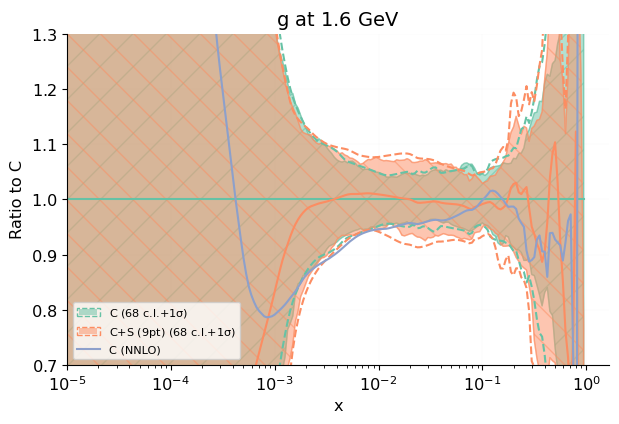
\includegraphics[scale=0.45]{mhous/plots/jplots/pdfscalespecs0_basespecs0_pdfnormalize0_plot_pdfs_g.png}
    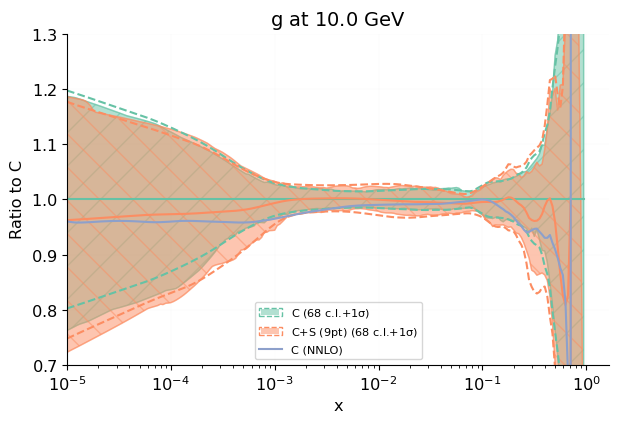
\includegraphics[scale=0.45]{mhous/plots/jplots/pdfscalespecs0_basespecs0_pdfnormalize0_plot_pdfs_g2.png}
         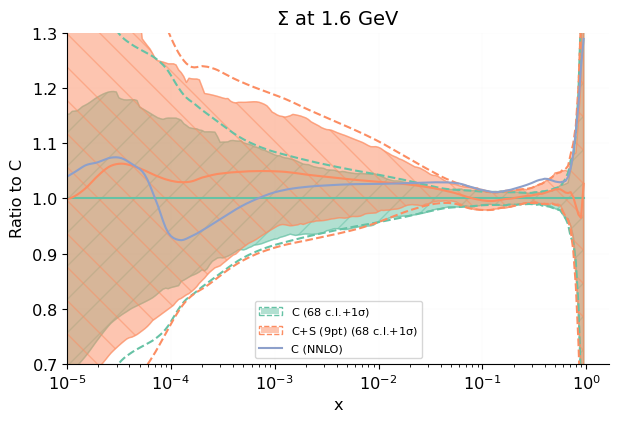
\includegraphics[scale=0.45]{mhous/plots/jplots/pdfscalespecs0_basespecs1_pdfnormalize0_plot_pdfs_Sigma.png}
            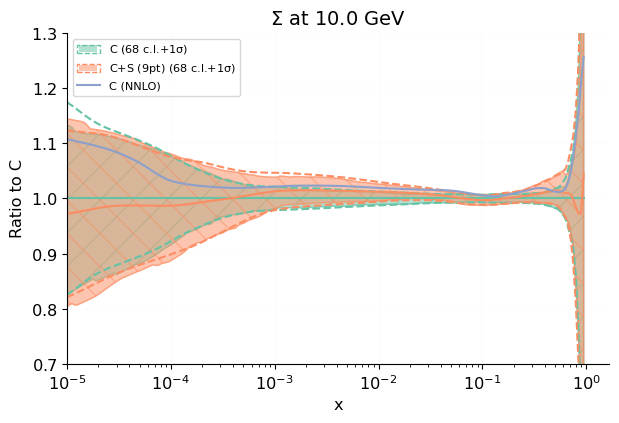
\includegraphics[scale=0.45]{mhous/plots/jplots/pdfscalespecs0_basespecs1_pdfnormalize0_plot_pdfs_Sigma2.png}
    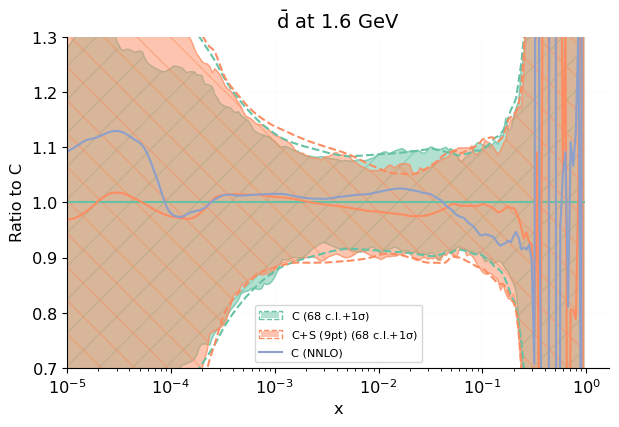
\includegraphics[scale=0.45]{mhous/plots/jplots/pdfscalespecs0_basespecs0_pdfnormalize0_plot_pdfs_bard.png}
         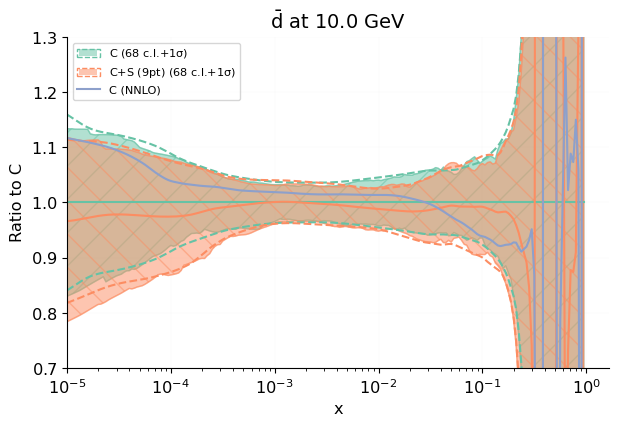
\includegraphics[scale=0.45]{mhous/plots/jplots/pdfscalespecs0_basespecs0_pdfnormalize0_plot_pdfs_bard2.png}
    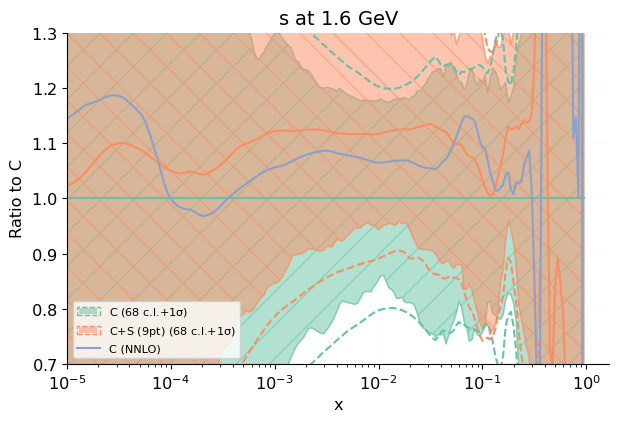
\includegraphics[scale=0.45]{mhous/plots/jplots/pdfscalespecs0_basespecs0_pdfnormalize0_plot_pdfs_s.png}
       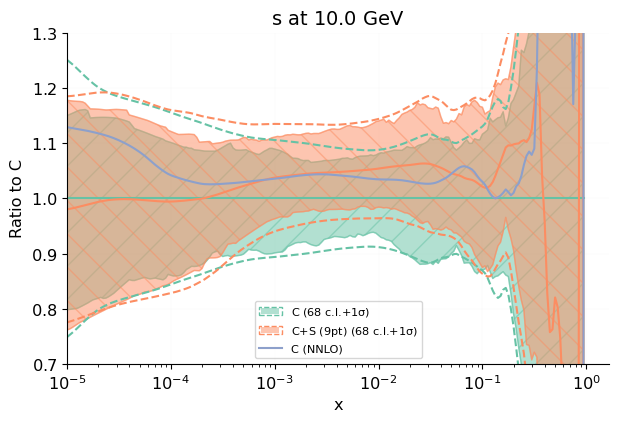
\includegraphics[scale=0.45]{mhous/plots/jplots/pdfscalespecs0_basespecs0_pdfnormalize0_plot_pdfs_s2.png}

   \caption{\small NLO PDFs based on $C$ (green) and $C+S^{\rm (9pt)}$ (orange) normalised
     to the former, alongside the central value of the NNLO fit based on $C$ (blue line).
     %
     Results are shown at $Q=1.6$ GeV (left column) and $Q=10$ GeV (right column). From top to bottom: gluon; total quark singlet;
     anti-down quark; strange quark.
    \label{fig:Global-NLO-CovMatTH} }
  \end{center}
\end{figure}
%%%%%%%%%%%%%%%%%%%%%%%%%%%%%%%%%%%%%%%%%%%%%%%%%%%%%%%%%%%%%%%%%%%%%%
%%%%%%%%%%%%%%%%%%%%%%%%%%%%%%%%%%%%%%%%%%%%%%%%%%%%%%%%%%%%%%%%%%%%%
\begin{figure}[H]
  \begin{center}
    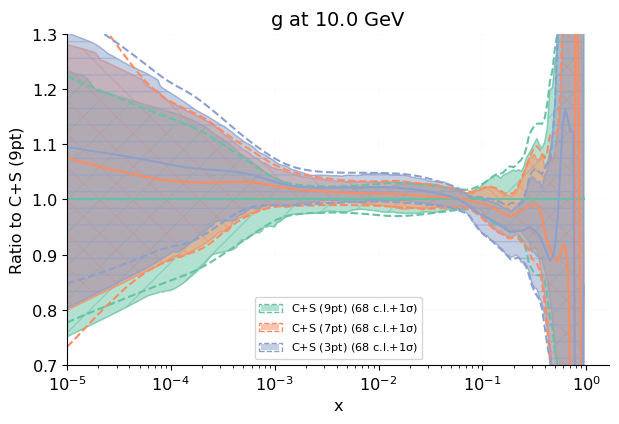
\includegraphics[scale=0.45]{mhous/plots/jplots/j2g.png}
    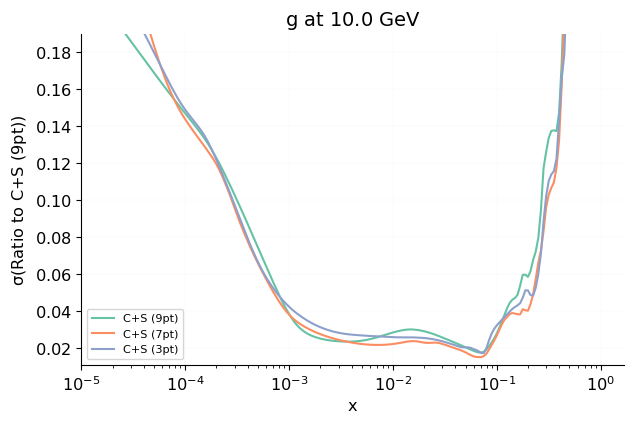
\includegraphics[scale=0.45]{mhous/plots/jplots/jeg.png}
        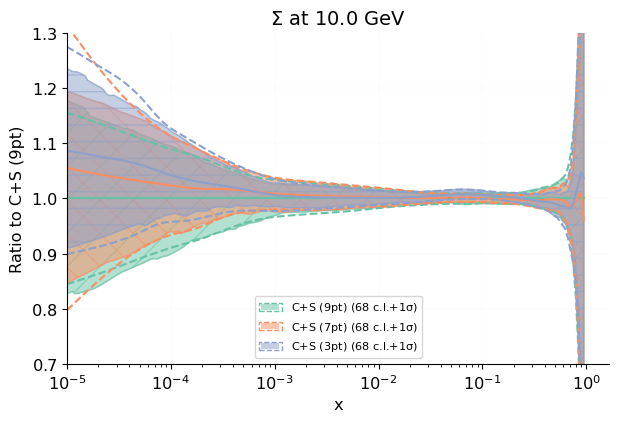
\includegraphics[scale=0.45]{mhous/plots/jplots/j2sig.png}
    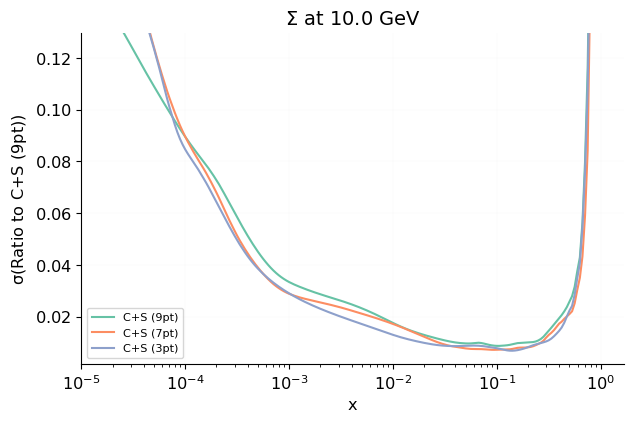
\includegraphics[scale=0.45]{mhous/plots/jplots/jesigma.png}
       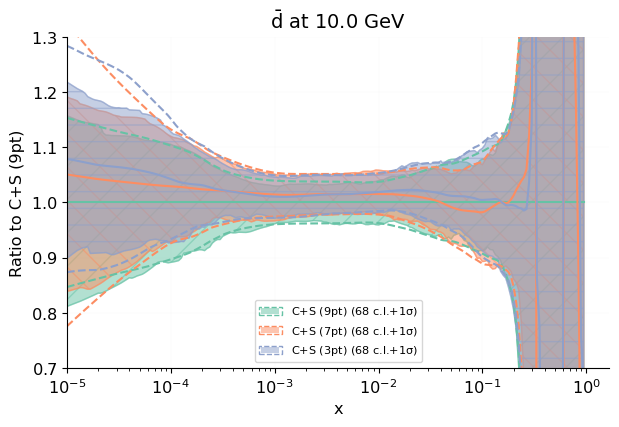
\includegraphics[scale=0.45]{mhous/plots/jplots/j2d.png}
    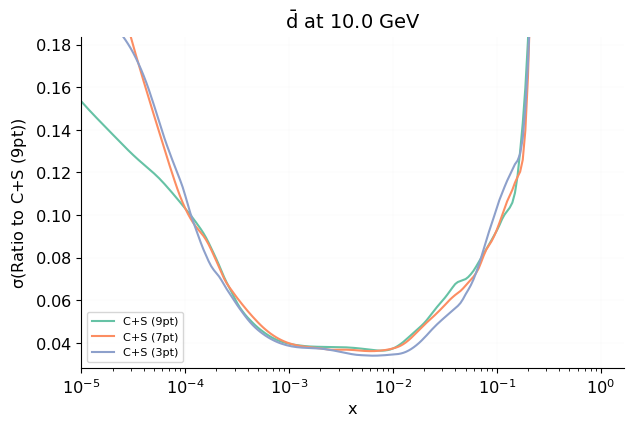
\includegraphics[scale=0.45]{mhous/plots/jplots/jed.png}
       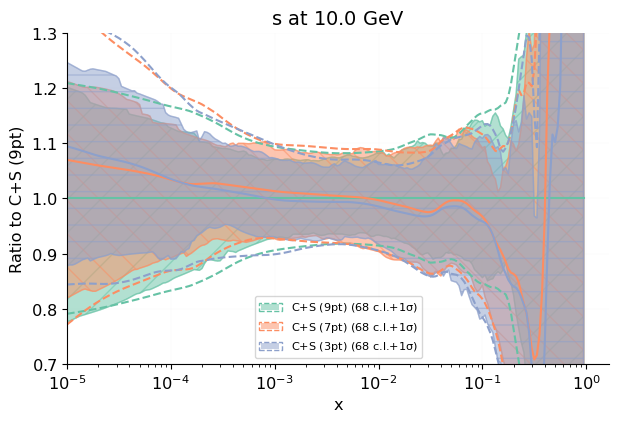
\includegraphics[scale=0.44]{mhous/plots/jplots/j2s.png}
    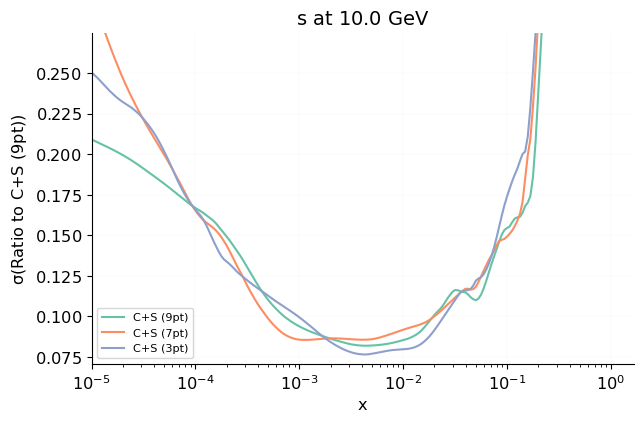
\includegraphics[scale=0.45]{mhous/plots/jplots/jes.png}
   \caption{\small Same as Fig.~\ref{fig:Global-NLO-CovMatTH} but comparing the 3- (blue), 7- (orange), and 9-point (green) prescriptions, normalised
     to 9-point. The right hand panel shows the 
     relative PDF uncertainties for clarity.
    \label{fig:Global-NLO-CovMatTH-prescriptions} }
  \end{center}
\end{figure}
%%%%%%%%%%%%%%%%%%%%%%%%%%%%%%%%%%%%%%%%%%%%%%%%%%%%%%%%%%%%%%%%%%%%%%
%%%%%%%%%%%%%%%%%%%%%%%%%%%%%%%%%%%%%%%%%%%%%%%%%%%%%%%%%%%%%%%%%%%%%
\begin{figure}[h]
  \begin{center}
    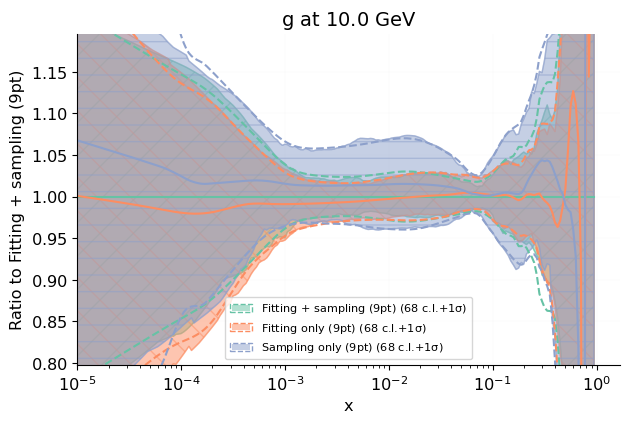
\includegraphics[scale=0.44]{mhous/plots/jplots/j3g.png}
        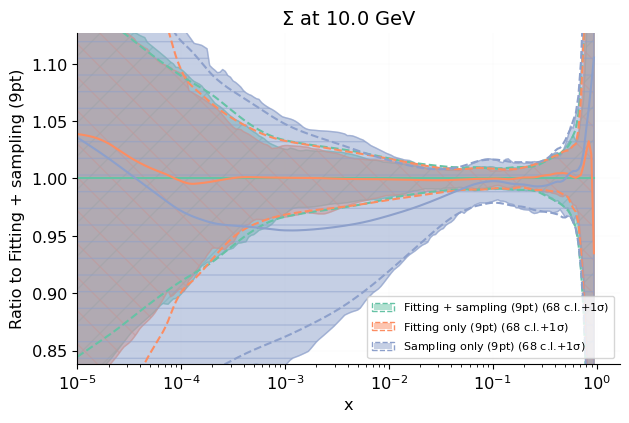
\includegraphics[scale=0.44]{mhous/plots/jplots/j3sigma.png}
       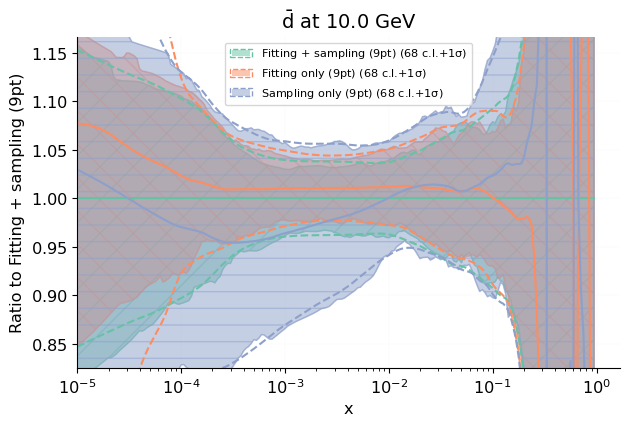
\includegraphics[scale=0.45]{mhous/plots/jplots/j3d.png}
       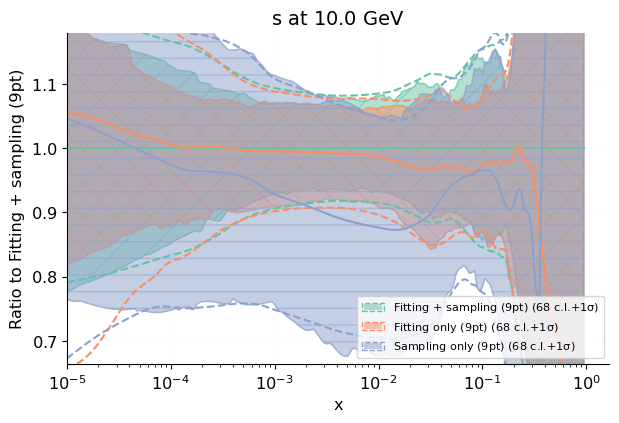
\includegraphics[scale=0.44]{mhous/plots/jplots/j3s.png}
   \caption{\small Same as Fig.~\ref{fig:Global-NLO-CovMatTH}, now comparing $C+S^{(\rm 9pt)}$ fit (green) with those in which
     the theory covariance matrix $S$ is included either in the $\chi^2$
     definition (orange) or in the generation of Monte Carlo replicas (blue), but not in both.
    \label{fig:Global-NLO-CovMatTH-tests} }
  \end{center}
\end{figure}
%%%%%%%%%%%%%%%%%%%%%%%%%%%%%%%%%%%%%%%%%%%%%%%%%%%%%%%%%%%%%%%%%%%%%%
\newpage
Finally we compare using $S$ in only fitting or sampling (Fig~\ref{fig:Global-NLO-CovMatTH-tests}). For sampling only, the PDF uncertainty increases dramatically, with poor fit quality, especially in the quark distributions. For fitting only, the central value is affected due to the change in relative weights of the datasets, such that it is similar to that for fitting + sampling. The uncertainty, however, shows only a very small change in the data region. This all arises because the inclusion of MHOUs in data generation cause the pseudodata broadness to increase dramatically, which is in turn balanced by a relaxation of tensions due to the inclusion of MHOUs in fitting. This has the effect of a sizeable shift in central values with only a small increase in uncertainties. 

\section{Overview}
\label{sec:overview}
We have presented the first PDFs with MHOUs included in their uncertainties, paving the way for the routine inclusion of theory uncertainties in future PDFs. This chapter has been primarily focussed on the formalism necessary for including MHOUs, and on the validation of the method. We find that scale variation appears to work well for this purpose, and that our prescriptions for combining scales are more successful and free from instabilities than the established ``envelope" techniques. It is also clear that there is scope for more complex scale variation techniques, particularly for the factorisation scale, which as a first step could be split into singlet and non-singlet variation. 

The PDFs detailed in this chapter, along with PDFs with varied scales, are available in {\tt LHAPDF} format~\cite{Buckley:2014ana} from the NNPDF website:

\begin{center}
 \href{http://nnpdf.mi.infn.it/nnpdf3-1th/}{\tt http://nnpdf.mi.infn.it/nnpdf3-1th/}
\end{center}

It now remains to investigate the impact of including MHOUs in PDFs on phenomenology, that is, in using them to compute predictions for cross-sections. For this some thorough analysis is required to address the potential ``double counting" of theory uncertainties, where they are included both in the PDF and in the hard cross-section. We will address this in considerable detail in Chapter \ref{chapter:correlations}. First, however, we will look at one other important form of theory uncertainties: those due to nuclear effects.